\documentclass[12pt]{report}
\usepackage{amssymb,amsthm,makeidx,verbatim,latexsym,amsfonts,graphicx,mathrsfs}
\usepackage{nomencl,tikz,caption,subcaption,enumitem,multicol,natbib,bm,lscape}
\usepackage{tasks,comment,tocloft,url,float,pdfpages,tabularx,booktabs,longtable}
\usepackage{bbm}
\usepackage[hidelinks]{hyperref}
\usepackage[tbtags]{amsmath}
\usepackage{colortbl,multirow,mathtools}
\usetikzlibrary{shapes.multipart}
\usetikzlibrary{positioning,calc,shapes.geometric,arrows,matrix,fit,backgrounds,intersections}
\makenomenclature
\renewcommand{\nomname}{Notations}


\newtheorem{defn}{Definition}[section]
\newtheorem{thm}{Theorem}[section]
\newtheorem{pro}{Proposition}[section]
\newtheorem{corr}{Corollary}[section]
\newtheorem{lemma}{Lemma}[section]
\newtheorem{rem}{Remark}[]
\newtheorem{exm}{Example}[]
\numberwithin{equation}{section}

\hfuzz=20.002pt
\vfuzz=20pt
\hbadness=2000
\vbadness=\maxdimen

\renewcommand{\baselinestretch}{1.5}
\textheight 9truein \hoffset -2cm \voffset -2cm \textwidth 6.6truein
\evensidemargin 2cm
\DeclareMathOperator*{\argmax}{arg\,max}
\DeclareMathOperator*{\argmin}{arg\,min}

\DeclarePairedDelimiter\ceil{\lceil}{\rceil}
\DeclarePairedDelimiter\floor{\lfloor}{\rfloor}

\renewcommand{\tabcolsep}{0.3cm}
\renewcommand{\arraystretch}{1.1}
\newcommand{\otoprule}{\midrule[\heavyrulewidth]}
\newcolumntype{A}{>{$}c <{$}}

\begin{document}

\begin{titlepage}
\pagenumbering{roman}
\setcounter{page}{0}
\addcontentsline{toc}{chapter}{Title Page}
\begin{center}
\begin{large}
\textbf{MACHINE LEARNING WITH APPLICATIONS \vskip 0.2cm IN AGRICULTURE}
\end{large}
\vskip 1.5cm 
BY
\vskip 1.5cm 
Abiodun Uthman ALLISON
\vskip 0.1cm 
B.Sc. Mathematics \\ (Federal University of Agriculture, Abeokuta)
\vskip 0.1cm 
\textbf{Matric. Number: 204603}
\vskip 1.5cm 
A Project submitted to the Department of  Mathematics\\
Faculty of Science\\
University of Ibadan, Ibadan\\
Nigeria
\vskip 1.5cm 
In Partial Fulfilment of the Award of Master of Science (M.Sc.) in Mathematics\\
In The Department of Mathematics, Faculty of Science\\
University of Ibadan, Ibadan\\
Nigeria
\vskip 1.5cm 
\flushright FEBRUARY, 2021
\end{center}
\end{titlepage}

\newpage
\pagenumbering{roman}
\newpage\addcontentsline{toc}{chapter}{Certification}
\section*{\centering Certification}
I certify that this project was carried out by {\bf ABIODUN UTHMAN ALLISON} \textbf{(Matric No. 204603)}, in the Department of Mathematics, Faculty of Science, University of Ibadan, under my supervision.
\vskip 2.5cm
\begin{center}
\tikz \draw[-] (0,0) -- (8,0);\vskip 0.2cm
\textbf{(Supervisor)}\vskip 0.2cm
\textbf{Professor G.O.S. Ekhaguere}\vskip 0.2cm
\textbf{Ph.D (London)}
\vskip 0.2cm
\textbf{Department of Mathematics,\vskip 0.2cm
University of Ibadan, Nigeria}
\end{center}


\newpage
\addcontentsline{toc}{chapter}{Dedication}
\section*{\centering Dedication}
Dedicated to Mulikat Allison.
%This project is dedicated to my parents. I am deeply indebted to my supervisor, Dr P.O Arawomo, without whose guidance and support this work will not have  I am deeply indebted to my supervisor, Dr P.O Arawomo, without whose guidance and support this work will not have come to light. I am thankful for the guidance and advice you gave me from the inception of the work to its completion, may God bless you abundantly.

\newpage 
\addcontentsline{toc}{chapter}{Acknowledgement}
\section*{\centering Acknowledgement}
%I bless God almighty for the strength and  wisdom to carry out this project work. I am deeply indebted to my supervisor, Professor G.O.S. Ekhaguere, without whose guidance and support this work will not have come to light. I am thankful for the guidance and advice you gave me from the inception of the work to its completion, may God bless you abundantly.

%It is a pleasure to acknowledge the impact of the distinguished Professors and members of staff of the department in my Mathematical journey. I am infinitely thankful to my parents, and my for your constant support and prayers. To my colleagues in the department, I thank God our paths did cross and I say ``a beautiful thank you" for your ceaseless help and support throughout the program, I couldn't ask for better. 

I give all glory, honour and adoration to Almighty Allah who brought me to this stage of my life. I owe a million debt of gratitude to my ever-loving parents, Mr Jamiu Allison and Mrs Mulikat Allison for their relentless supports toward the success of my education. I also appreciate my ever loving siblings for their continuous support.

Also my profound appreciation goes to my supervisor, Professor G.O.S. Ekhaguere, for his patience, guidance and helpful suggestions, thank you sir. In the same vein, my unmeasured gratitude goes to all the distinguished Professors and members of staff of the Department of Mathematics for their unrelenting effort. I also acknowledge my friends and my course mates for their love and support, I say thank you all.

%My special thanks goes to the Head of Department, Dr. Deborah Ajayi for her support, advice and tolerance towards the students of the mathematics department.




\newpage
\addcontentsline{toc}{chapter}{Abstract}
\section*{\centering Abstract}
Current rapid development in Artificial Intelligence (AI) provides a vast selection of high quality tools to solve complex problems in more efficient ways than before. As a consequence, many fields of science and engineering are starting to explore AI tools, especially Deep Learning (DL) models for computer vision, audio and video understanding, speech recognition and decision making. In this project, we studied a type of deep learning model - Convolutional Neural Networks (CNNs), starting with a basic Machine Learning algorithm - Logistic Regression, moving on to building blocks of Neural Networks and method of training and optimising neural network models. We then implemented three different CNN architectures; a base model, VGG16 and ResNext-50, to classify different plant diseases using healthy and diseased leaf images. The best performing model was ResNext-50 with $98\%$ accuracy. 




\newpage \addcontentsline{toc}{chapter}{Table of Contents}
\renewcommand*{\contentsname}{\centering \Large TABLE OF CONTENTS}
\tableofcontents 

\newpage \addcontentsline{toc}{chapter}{List of Figures}
\renewcommand{\cftfignumwidth}{6em}
\renewcommand{\cftfigpresnum}{Figure }
\listoffigures

\newpage \addcontentsline{toc}{chapter}{List of Tables}
\renewcommand{\cfttabnumwidth}{6em}
\renewcommand{\cfttabpresnum}{Table }
\listoftables


\newpage
\pagenumbering{arabic} 

\chapter{Introduction}
\setcounter{section}{-1}   


\section{Introduction}
Agriculture, for decades, had been associated with the production of essential food crops. At present, agriculture also includes forestry, dairy, fruit cultivation, poultry, bee keeping, mushroom etc. Today, processing, marketing, and distribution of crops and livestock products are all acknowledged as part of current agriculture. Thus, agriculture could be referred to as the production, processing, promotion and distribution agricultural products. Agriculture plays a critical role in the entire life of a given economy. In addition to providing food and raw materials, agriculture also provides employment opportunities, government revenue, food security, significance in transport among other things. 

Machine learning is the scientific study of algorithms and statistical models that computer systems use to perform a specific task without using explicit instructions, relying on patterns and inference instead. Machine learning algorithms build a mathematical model based on training data (a sample data), in order to make predictions or decisions without being explicitly programmed to perform the task. Machine learning algorithms are used in a wide variety of applications, such as email filtering, computer vision, and stock market prediction, where it is difficult  to develop a conventional algorithm for effectively performing the task.  

Plant health and food safety are closely linked. The Food and Agriculture Organization of the United Nations (FAO) estimates that pests and diseases lead to the loss of $20-40\ \%$ of global food production, constituting a threat to food security (Food and Agriculture Organization of the United Nation, International Plant Protection Convention, 2017). Use of pesticides has been a way of protecting crops from these infestations and has been one of the factors behind the increase in food production since the 1950s, enabling it to meet the needs of a growing population {\cite{cooper}}. However, the use of such substances is not environmentally harmless. Applying these substances negatively impacts biodiversity, including insect, bird, and fish populations, as well as soil, air, and water quality {\cite{kaur}}; {\cite{bayo}}; {\cite{Knillmann}}. Their use also constitutes a risk to human health, with both acute and chronic effects {\cite{sanborn}}; {\cite{KIM2017525}}. Plant diseases are not only a threat to food security at the global scale, but can also have disastrous consequences for smallholder farmers whose livelihoods depend on healthy crops.

Computer vision, and object recognition in particular, has made tremendous advances in the past few years. The PASCAL Visual Object Classes (VOC) challenge {\cite{Everingham}}, established in 2005, which set the precedent for standardized evaluation of recognition algorithms in the form of yearly competitions, and more recently the Large Scale Visual Recognition Challenge (ILSVRC) {\cite{Russakovsky}} based on the ImageNet dataset {\cite{Deng}} have been widely used as benchmarks for numerous visualization-related problems in computer vision,including object classification. In 2012, a large, deep convolutional neural network achieved a top-5 test error (the fraction of test images for which the correct label is not among the five labels considered most probable by the model) rate of $15.3\ \%$, almost halved the error rate compared
to $26.2\ \%$ achieved by the second-best entry, at the ILSVRC 2012 image classification competition for the classification of $15$ million images into $22$ thousand possible categories {\cite{Krizhevsky}}. In the following years, various advances in deep convolutional neural networks lowered the top-5 error rate to $3.57\ \%$ {\cite{He2015DeepRL}}; {\cite{Szegedy}}, $3.03\ \%$ {\cite{Xie}}, $2.251\ \%$ {\cite{Hu2017SqueezeandExcitationN}}.

In image classification problems with lots of classes, a considerable amount of sample size is required to train deep learning models. But with increase in the amount of data available, the development of Graphical Processing Unit (GPU) parallel computing ability, and cloud computing, there have a seen a significant improvement in training deep learning models. This project work deals with the application of machine learning (deep learning in particular) algorithms in the areas of plant disease recognition and  in agriculture.

\section{Basic Definitions and Results}
In what follows in the section, we give some preliminary definitions and results which will aid in the understanding of machine leaning and deep learning.

\subsection{Tensor and Vectorisation}
In this project, we use a symbol shown in boldface to represent a vector, for example, $\bm{x} \in \mathbb{R}^D$ is a column vector with $D$ elements; a capital letter to denote a matrix, for example, $X \in \mathbb{R}^{H\times W}$ is a matrix with $H$ rows and $W$ columns. The vector $\bm{x}$ can also be viewed as a matrix with $1$ column and $D$ rows.

These concepts can be generalised to higher order matrices, i.e., tensors. For example, $\bm{x} \in \mathbb{R}^{H\times W\times D}$ is an order 3 tensor. It contains $HWD$ elements, and each of them can be indexed by an index triplet $(i,j,d)$, with $0\leq i < H$, $0\leq j < W$, and $0\leq d < D$. Another way to view an order $3$ tensor is to treat it as containing $D$ channels of matrices. Every channel is a matrix with size $H \times W$. The first channel contains all the numbers in the tensor that are indexed by $(i,j,0)$. When $D=1$, an order $3$ tensor reduces to a matrix.

A scalar value is an order $0$ tensor; a vector is an order $1$ tensor; and a matrix is a second order tensor. A color image is in fact an order $3$ tensor, if a color image is stored in the RGB format, it has $3$ channels (for R, G and B, respectively), and each channel is a $H\times W$ matrix that contains R (or G, or B) values of all pixels. It is beneficial to represent images (or other types of raw data) as a tensor, this helps keep the color information of the images as color is very important in various image based learning and recognition problem. 

Given a tensor, we can arrange all the numbers inside it into a long vector, following a pre-specified order. In order to vectorise an order 3 tensor, we would vectorise its first channel (which is a matrix), then the second channel, $\hdots$,  till all channels are vectorised. The vectorisation of the order 3 is then the concatenation of the vectorisation of all the channels in this order. This method can be applied to vectorise tensors of order greater than 3. For example, in Python 3.7,  \texttt{numpy.reshape(A.shape[0]*A.shape[1]*A.shape[2],1)} converts  tensor $\bm{A}$ into a column vector in the row-first order. 

\subsection{Vector Calculus and the Chain Rule}
Suppose $z \in \mathbb{R}$ is a scalar and $\bm{y} \in \mathbb{R}^H$ is a vector. IF $z$ is a function of $\bm{y}$, the partial derivative of $z$ with respect $\bm{y}$ is a vector, defined as 
\begin{equation}\label{eqn:2}
{\left[\dfrac{\partial z}{\partial \bm{y}}\right]}_i = \dfrac{\partial z}{\partial y_i}
\end{equation} 
In other words, $\frac{\partial z}{\partial \bm{y}}$ is a vector having the same size as $\bm{y}$, and its $i$-th element is $\frac{\partial z}{\partial y}$. We also note that $\frac{\partial z}{\partial \bm{y}^T} = (\frac{\partial z}{\partial \bm{y}})^T$.

Furthermore, suppose $\bm{x}\in \mathbb{R}^W$ is another vector, and $\bm{y}$ is a function of $\bm{x}$. Then, the partial derivative of $\bm{y}$ with respect $\bm{x}$ is defined as
\begin{equation}\label{eqn:3}
{\left[\dfrac{\partial \bm{y}}{\partial \bm{x}^T}\right]}_{ij} = \dfrac{\partial y_i}{\partial x_j}
\end{equation} 
This partial derivative is $H \times W$ matrix, whose entry at the intersection of the $i$-th row and $j$-th column is $\frac{\partial y_i}{\partial x_j}$.

In a chain-like argument, we see that $z$ is a function of $\bm{x}$. The chain rule can be used to compute $\frac{\partial z}{\partial \bm{x}^T}$ as 
\begin{equation}\label{eqn:4}
\dfrac{\partial z}{\partial \bm{x}^T} = \dfrac{\partial z}{\partial \bm{y}^T} \dfrac{\partial \bm{y}}{\partial \bm{x}^T}
\end{equation}
Since $\frac{\partial z}{\partial \bm{x}^T}$ is a $1\times H$ matrix and $\frac{\partial \bm{y}}{\partial \bm{x}^T}$ is an $H \times W$ matrix, the matrix multiplication in ~\eqref{eqn:4} is valid, and the result would be a row vector with $W$ elements, which matches the dimensionality of $\frac{\partial z}{\partial \bm{x}^T}$.

\subsection{Binomial Distribution}
Consider a random experiment which consists of $n$ independent trials, such that for each trial they are two possible outcomes; success and failure. Let $P(\text{success})=p$ and $P(\text{failure})=1-p$, and $X$ the random variable with $x$ number of successes, then the binomial distribution is defined as 
\begin{equation}\label{binomial}
B(n,p) = \binom{n}{x}p^x(1-p)^{n-x}, \quad 0\leq x \leq n 
\end{equation} 
$p^x$ computes the probability of achieving the the demanded $x$ success over all trials, and $(1-p)^{n-x}$ computes the probability of the rest of the trials being failure.  

\subsection{Norms}\label{sub:norm}
The norm function is used to measure the size of vectors in machine learning. Formally, the $L^p$ norm is given by 
\begin{equation}\label{eqn:lp-norm}
\|\bm{x}\|_p = \left( \sum_i|\bm{x}_i|^p \right)^{\frac{1}{p}}
\end{equation} 
for $p\in\mathbb{R}$, $p\geq 1$.

Norms, including the $L^p$ norm, are functions mapping vectors to non-negative real numbers. On an intuitive level, the norm of a vector $\bm{x}$ measures the distance from the origin to the point $\bm{x}$. A norm is a map $\|.\|:\bm{X}\rightarrow \mathbb{R}^+$ that satisfies the following properties:
\begin{itemize}
\item $\|x\| \geq 0, \quad \forall\;\bm{x}\in\bm{X} \quad$ (non-negativity)
\item $\|\bm{x}\| = 0$ if and only if $\bm{x}=0$
\item $\forall\; \alpha\in \mathbb{R}$, $\|\alpha \bm{x}\| = |\alpha|\|\bm{x}\|\quad$ (positive homogeneous)
\item $\|\bm{x}+\bm{y}\| \leq \|\bm{x}\| + \|\bm{y}\| \quad \forall\; \bm{x},\bm{y}\in\bm{X}\quad$ (triangle inequality)
\end{itemize}
The $L^2$ norm, with $p = 2$, is known as the {Euclidean norm}, which is simply the Euclidean distance from the origin to the point identified by $\bm{x}$. The $L^2$ norm is used to keep a model less more complex by keeping the coefficients of the model small. It is given by:
\begin{equation}\label{eqn:l2-norm}
\|\bm{x}\|_2 = \sqrt{\sum_i x_i^2}
\end{equation} 
In several machine learning applications, it is important to discriminate between elements that are exactly zero and elements that are small but nonzero. In these cases, we use the $L^1$ norm, which is given by:
\begin{equation}\label{eqn:l1-norm}
\|\bm{x}\| = \sum_i |x_i|
\end{equation}
One other norm that commonly arises in machine learning is the $L^\infty$ norm, also known as the {max norm}. This norm simplifies to the absolute value of the element with the largest magnitude in the vector, it is given by:
\begin{equation}\label{eqn:max-norm}
\|\bm{x}\|_\infty = \max_i |x_i|
\end{equation}

Sometimes we may also wish to measure the size of a matrix. In the context
of deep learning, the most common way to do this is with the {Frobenius norm}:
\begin{equation}\label{eqn:fro-norm}
\|\bm{A}\|_F = \sqrt{\sum_{i,j} A_{i,j}^2}
\end{equation} 
which is analogous to the $L^2$ norm of a vector, where $\bm{A}$ is a matrix and $A_{i,j}$ are values of $\bm{A}$.

\subsection{Convex Optimisation}
Consider the general {constrained} optimisation problem 
\begin{equation}\label{eqn:optimize}
\begin{array}{ll}
\text{minimize} & f(x)  \\
\text{subject to} & \bm{x} \in D \subset \mathbb{R}^n \\
\end{array}
\end{equation}
The function $f:\mathbb{R}^n \rightarrow \mathbb{R}$ that we wish to minimise is a real valued function called {objective function}. The vector $\bm{x}=(x_1,x_2,\hdots,x_n)\in \mathbb{R}^n$ is an $n$-vector of independent variables $x_1,x_2,\hdots,x_n$ which are called {decision variables}, the set $D \subset \mathbb{R}$ is called the {constrained or feasible set}. The optimisation problem involves obtaining the best vector of decision variables over all possible vectors in $D$. The vector here is the minimizer of $f$ over $D$. If $D=\mathbb{R}^n$, the problem \eqref{eqn:optimize} is called an {unconstrained} optimisation problem.
\begin{defn} 
\normalfont
(Global minimum).
Let $\bm{x}_0 \in D \subseteq \mathbb{R}^n$ and $f:D \rightarrow \mathbb{R}$ such that $D \neq \emptyset$. If $f(\bm{x}) \geq f(\bm{x}_0) \;  \forall \; \bm{x} \in D$, then point $\bm{x}_0$ is called a global minimum point.
\end{defn}
\begin{defn} 
\normalfont
(Local minimum).
Let $\bm{x}_0 \in D \subseteq \mathbb{R}^n$ and $f:D \rightarrow \mathbb{R}$ with $D \neq \emptyset$. If $f(\bm{x}) \geq f(\bm{x}_0) \;  \forall \; \bm{x} \in D \cap \mathcal{B}_{\bm{x}_0}(\varepsilon),\; \varepsilon>0$, then point $\bm{x}_0$ is called a local minimum point. ($\mathcal{B}_{\bm{x}_0}(\varepsilon) = \{ \bm{x} \in \mathbb{R}^n: \| \bm{x}-\bm{x}_0<\varepsilon\|\}$)
\end{defn}
\begin{defn} 
\normalfont
(Argument of the minimum).
Given an arbitrary set $X$,  and a function, $f\colon X\rightarrow Y$, the argument of the minimum (written $\arg\min$) over some subset, $S$, of $X$ is defined by
\[ \underset{x \in S}{\arg \min } f(x):=\{x \in S | \; \forall y \in S: f(y) \geq f(x)\}
\]
They are points $x$ for which $f(x)$ attains its smallest value. 
\end{defn}
\begin{defn} 
\normalfont
(Local and global minimizer).
Let $f:D \rightarrow \mathbb{R}$. If $\exists \  \varepsilon > 0$ such that  $f(x) \geq f(x_0) \  \forall \ x \in D\backslash \{x_0\}$, and $\forall \  \|x-x_0\|<\varepsilon$.  Then the point $x_0 \in D$ is a local minimizer of $f$ over $D$. If $f(x) \geq f(x_0) \  \forall \ x \in D\backslash \{x_0\}$, then  $x_0 \in D$ is a global minimizer of $f$ over $D$
\end{defn}
\begin{defn}
\normalfont
(Convex set).
Let $\bm{x}_1,\bm{x}_2 \in D \neq \emptyset$ and $0\leq \varphi \leq 1$. Then $D$ is convex provided that 
\[
\varphi \bm{x}_1 + (1-\varphi)\bm{x}_2 \in D 
\]
\end{defn}
\begin{defn}
\normalfont
(Convex functions).
Let $f:\mathbb{R}^n\rightarrow\mathbb{R}$ be defined on a non empty set $D\subseteq\mathbb{R}^n$. Then $f$ is convex on $D$ if $\forall \; \bm{x}_1,\bm{x}_2 \in D$ and $\varphi \in [0,1]$
\begin{equation}\label{eqn:convex_fxn}
f(\varphi \bm{x}_1 + (1-\varphi)\bm{x}_2) \leq \varphi f(\bm{x}_1) + (1-\varphi)f(\bm{x}_2)
\end{equation}
$f$ is strictly convex if the inequality is always strict, i.e. if $\bm{x}_1\neq \bm{x}_2$ implies that
\begin{equation}\label{eqn:convex_strict}
f(\varphi \bm{x}_1 + (1-\varphi)\bm{x}_2) < \varphi f(\bm{x}_1) + (1-\varphi)f(\bm{x}_2)
\end{equation}
$f$ is concave if $-f$ is convex. If the graph of a convex function is drawn, any line joining any two points in the graph would be above the graph. 
\end{defn}
\begin{defn}
\normalfont
(Strong convexity).
A differentiable function $f:\mathbb{R}^n\rightarrow\mathbb{R}$ is said to be $\mu$-strongly convex if:
\begin{equation}\label{eqn:strong_convex}
f(\bm{y}) \geq f(\bm{x}) + \nabla f(\bm{x})^T (\bm{y}-\bm{x}) + \frac{\mu}{2} \| \bm{y}-\bm{x} \|^2
\end{equation}
for some $\mu > 0$ and $\forall \; \bm{x},\bm{y} \in \mathbb{R}^n$. Strong convexity does not necessarily require the function to be differentiable, and the gradient is replaced by the subgradient when the function is non-smooth. The set of subgradients is the subdifferential $\partial f(\bm{x})$, given by: 
\begin{equation}\label{eqn:subgradient}
\partial f(\bm{x}) = \{\bm{g}: f(\bm{y}) \geq f(\bm{x})+ \bm{g}^T (\bm{y}-\bm{x}), \; \forall \bm{y}\}
\end{equation}
where $\bm{g} \in \mathbb{R}^n$ is the subgradient at point $\bm{x}$. 
\end{defn}
\begin{pro}
\normalfont
The following conditions are all equivalent to the condition that a differentiable function $f$ is strongly-convex with constant $\mu > 0$.
\begin{enumerate}[label=(\alph*)]
\item $f(\bm{y})\ge f(\bm{x})+\nabla f(\bm{x})^T(\bm{y}-\bm{x})+\dfrac{\mu}{2}\lVert \bm{y}-\bm{x} \rVert^2,~\forall \bm{x}, \bm{y}$
\item $g(\bm{x}) = f(\bm{x})-\dfrac{\mu}{2} \| \bm{x} \|^2 \text{ is convex }\;\forall \;\bm{x}$
\item $(\nabla f(\bm{x}) - \nabla f(\bm{y}))^T(\bm{x}-\bm{y}) \ge \mu \lVert \bm{x}-\bm{y}\rVert^2,~\forall \; \bm{x}, \bm{y}$
\item $f(\varphi \bm{x}+ (1-\varphi) \bm{y}) \le \varphi f(\bm{x}) + (1-\varphi) f(\bm{x}) - \dfrac{\varphi (1-\varphi)\mu}{2} \| \bm{x}-\bm{y} \|^2,~\varphi \in [0,1]$
\end{enumerate}
\end{pro}
\begin{comment}
\begin{lemma}
\normalfont
For a continuously differentiable function $f$, the following conditions are all implied by strong convexity of $f$.
\begin{enumerate}[label=(\alph*)]
\item 
\end{enumerate}
\end{lemma}
\end{comment}
\begin{lemma}
\normalfont
If $f$ is twice continuously differentiable, then it is strongly convex with parameter $\mu > 0$ if and only if $\nabla^2 f(\bm{x}) \succeq \mu I,\;\forall\;\bm{x}$, where $I$ is the identity matrix. This means that the matrix $\nabla^2 f(\bm{x}) - \mu I$ is positive semi definite.
\end{lemma}
\begin{pro}\label{pro:sum}
\normalfont
Let $h=f+g$ where $f$ is strongly convex function and $g$ is a convex function, then $h$ is a strongly convex function.
\end{pro}
\begin{proof}
For $\varphi \in [0,1]$, $\bm{x},\bm{y} \in \mathbb{R}^n$, and $\mu > 0$, we have
\begin{align*}
h(\varphi \bm{x} + (1-\varphi)\bm{y}) &= f(\varphi \bm{x} + (1-\varphi)\bm{y}) + g(\varphi \bm{x} + (1-\varphi)\bm{y})\\
	& \le \varphi f(\bm{x}) + (1-\varphi)f(\bm{y}) - \frac{\mu \varphi (1-\varphi)}{2}\|\bm{x}-\bm{y}\|^2 + \varphi g(\bm{x}) + (1-\varphi)g(\bm{y})\\
	& = \varphi [f(\bm{x})+g(\bm{x})] + (1-\varphi) [f(\bm{y})+g(\bm{y})] - \frac{\mu \varphi (1-\varphi)}{2}\|\bm{x}-\bm{y}\|^2 \\
	& = \varphi h(\bm{x}) + (1-\varphi) h(\bm{y}) - \frac{\mu \varphi (1-\varphi)}{2}\|\bm{x}-\bm{y}\|^2 
\end{align*} 
\end{proof}
\begin{thm}\label{thm:local_is_global}
\normalfont
Any local minimum of a convex function $f:\mathbb{R}^n\rightarrow\mathbb{R}$ is also a global minimum.
\end{thm}
\begin{lemma}\label{lemma:sum}
\normalfont
The weighted sums of $m$ convex functions $f_1,f_2,\hdots,f_m$
\[ f := \sum_{i=1}^m \alpha_i f_i \]
is convex as long as the weights $\alpha_1,\alpha_2,\hdots,\alpha_m$ are non-negative. 
\end{lemma}
\begin{proof}
By convexity of $f_1,f_2,\hdots,f_m$, for any $\bm{x}_1,\bm{x}_2 \in \mathbb{R}^m$ and $\varphi \in [0,1]$
\[
\begin{aligned} 
f(\varphi \bm{x}_1+(1-\varphi) \bm{x}_2) &=\sum_{i=1}^{m} \alpha_{i} f_{i}(\varphi \bm{x}_1+(1-\varphi) \bm{x}_2) \\ 
	& \leq \sum_{i=1}^{m} \alpha_{i}\left(\varphi f_{i}(\bm{x}_1)+(1-\varphi) f_{i}(\bm{x}_2)\right) \\ 
	&=\varphi f(\bm{x}_1)+(1-\varphi) f(\bm{x}_2) 
\end{aligned}
\]
which shows that $f$ is convex.
\end{proof}
\begin{defn}
\normalfont (Quadratic from of a symmetric matrix).
The quadratic form of an $n\times n$ symmetric matrix $\bm{A}$, denoted by $Q_{\bm{A}}(\bm{x})$ is a function $f:\mathbb{R}^n\rightarrow \mathbb{R}$ given by $f(\bm{x})=\bm{xQx^T}$, $\bm{x}\in\mathbb{R}^n$. $\bm{A}$ is
\begin{itemize}
\item positive definite, if $Q_{\bm{A}}(\bm{x}) > 0 \; \forall \; \bm{x}\in\mathbb{R}^n$
\item positive semi-definite, if $Q_{\bm{A}}(\bm{x}) \geq 0 \; \forall \; \bm{x}\in\mathbb{R}^n$
\item negative definite, if $Q_{\bm{A}}(\bm{x}) < 0 \; \forall \; \bm{x}\in\mathbb{R}^n$
\item negative semi-definite, if $Q_{\bm{A}}(\bm{x}) \leq 0 \; \forall \; \bm{x}\in\mathbb{R}^n$
\end{itemize}
\end{defn}
\begin{defn}
\normalfont
(Hessian matrix).
Suppose $f:\mathbb{R}^n\rightarrow\mathbb{R}$, $\bm{x}\in\mathbb{R}^n$. If all second partial derivatives of $f$ exist and are continuous over the domain of the function (i.e. $f\in C^2(dom\; f)$), then the Hessian matrix $\nabla^2(f(\bm{x}))$ of $f$ is a symmetric $n\times n$ matrix, defined as:
\begin{equation}
\nabla^2 f(\bm{x})=\left[\begin{array}{cccc}
{\dfrac{\partial^{2} f}{\partial x_{1}^{2}}} & {\dfrac{\partial^{2} f}{\partial x_{1} \partial x_{2}}} & {\cdots} & {\dfrac{\partial^{2} f}{\partial x_{1} \partial x_{n}}} \\
 {\dfrac{\partial^{2} f}{\partial x_{2} \partial x_{1}}} & {\dfrac{\partial^{2} f}{\partial x_{2}^{2}}} & {\cdots} & {\dfrac{\partial^{2} f}{\partial x_{2} \partial x_{n}}} \\
  {\vdots} & {\vdots} & {\ddots} & {\vdots} \\ {\dfrac{\partial^{2} f}{\partial x_{n} \partial x_{1}}} & {\dfrac{\partial^{2} f}{\partial x_{n} \partial x_{2}}} & {\cdots} & {\dfrac{\partial^{2} f}{\partial x_{n}^{2}}}\end{array}\right]
\end{equation}
or, by stating an equation for the coefficients using indices $i$ and $j$:
\begin{equation}
\nabla^2 f(\bm{x}) = \left(\frac{\partial^{2} f}{\partial x_{i} \partial x_{j}}\right)_{1 \leq i, j \leq n}
\end{equation}
\end{defn}
\begin{thm}\label{thm:first_order}
\normalfont {(First order condition).}
Let $f:\mathbb{R}^n\rightarrow \mathbb{R}$, $D \subset \mathbb{R}^n$ a convex set. If $f\in C^1(D)$, then $f$ is convex if and only if for every $\bm{x},\bm{y} \in D$
\begin{equation}
f(\bm{y})  \geq  f(\bm{x}) + \nabla^T f(\bm{x}) (\bm{y}-\bm{x}) 
\end{equation}
\end{thm}
\begin{thm}\label{thm:second_order}
\normalfont {(Second order condition).}
Let $f:\mathbb{R}^n\rightarrow \mathbb{R}$. If $f\in C^2(dom \; f)$, then $f$ is convex if and only if for every $\bm{x}\in\mathbb{R}^n$, the Hessian matrix $\nabla^2 f(\bm{x})$ is positive semi-definite.
\end{thm}

\subsection{Rate of Convergence}
The speed at which a convergent sequence approaches its limit is called the rate of convergence of the sequence. Rate of convergence is of practical importance when working with a sequence of successive approximations for an iterative method, as then fewer iterations are needed to yield a useful approximation if the rate of convergence is higher. One of the key measures of performance of an algorithm is its rate of convergence. 
\begin{defn}
\normalfont
Let $\{\bm{x}_k\}$ be a sequence in $\mathbb{R}^n$ that converges to $x^*$. Then,
\begin{enumerate}[label=\roman*)]
\item $\{\bm{x}_k\}$ is said to converge {Q-linearly} to $x^*$ if there exists $\beta \in (0,1)$, such that 
\[
\frac{\|\bm{x}_{k+1}-x^*\|}{\|\bm{x}_{k}-x^*\|} \leq \beta 
\]
This means that the distance to the solution $x^*$ decreases at each iteration by at least a constant factor.
\item $\{\bm{x}_k\}$ is said to converge {Q-superlinearly} (i.e. faster than linearly) to $x^*$ if  
\[
\lim_{k\rightarrow\infty} \frac{\|\bm{x}_{k+1}-x^*\|}{\|\bm{x}_{k}-x^*\|} = 0
\]
\item $\{\bm{x}_k\}$ is said to converge {Q-sublinearly} (i.e. slower than linearly) to $x^*$ if  
\[
\lim_{k\rightarrow\infty} \frac{\|\bm{x}_{k+1}-x^*\|}{\|\bm{x}_{k}-x^*\|} = 1
\]
\item $\{\bm{x}_k\}$ converges with $p$-order of convergence  for $p>1$ if  
\[
\ \frac{\|\bm{x}_{k+1}-x^*\|}{\|\bm{x}_{k}-x^*\|^p} \leq M \quad \forall \; k \text{ sufficiently large}
\]
for some positive constant $M$ (not necessarily less than $1$). When $q=2$, the convergence is quadratic, cubic when $q=3$ and so on. 
\end{enumerate}
The $Q$ in the definition stands for quotient, because the definition uses the quotient between two successive errors. 
\end{defn}

\subsection{Logistic Sigmoid Function}\label{sub:lsf}
A sigmoid function is a bounded, differentiable, real function that is defined for all real input values and has a non-negative derivative at each point. It takes in a real number and outputs a number in range $(0,1)$, having a characteristic ``S''-shaped curve or sigmoid curve. A standard choice for a sigmoid function is the standard logistic function shown in Figure (\ref{fig:sig}) and defined by the formula
\begin{equation}\label{eqn:sigma}
 \sigma(x) = \dfrac{1}{1+e^{-x}}
\end{equation}
with the following properties 
\begin{figure}[htb!]
\centering 
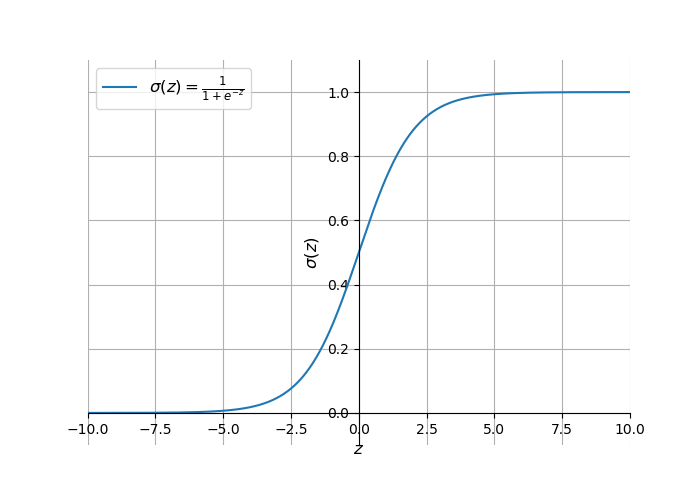
\includegraphics[scale=0.91]{png/sigmoid.png} 
\caption{Logistic sigmoid function}
\label{fig:sig}
\end{figure}
% We note that as $t \rightarrow \infty$, $e^{-t} \rightarrow 0$ thus $\sigma(t) \rightarrow 1$, also, as $t \rightarrow -\infty$, $e^{-t} \rightarrow \infty$ thus $\sigma(t) \rightarrow 0$. 
\begin{itemize}
\item Horizontal asymptotes exists at $\sigma(x)=0$ and $\sigma(x)=1$, and $y$-intercept at $(0,0.5)$
	\[
	\lim_{x \rightarrow \infty} \frac{1}{1+e^{-x}}=\frac{1}{1+\lim_{x \rightarrow 			\infty} e^{-x}}=\frac{1}{1+0}=1 \]
	\[ \lim_{x \rightarrow-\infty} \frac{1}{1+e^{-x}}=\frac{1}{1+\lim _{x \rightarrow-		\infty} e^{-x}}=\frac{1}{1+\lim_{x \rightarrow \infty} e^{x}}=0 \]
\item Symmetry property
	\begin{equation}\label{eqn:sigma1}
	\sigma(x) + \sigma(-x) = 1
	\end{equation}
	\[
	\frac{1}{1+e^{-x}}+\frac{1}{1+e^{-(-x)}}=\frac{e^{x}}{e^{x}+1}+\frac{1}{e^{x}+1}=1
	\]

\item Its derivative can be derived thus 
	\begin{equation}\label{eqn:sigma2}
	\begin{split}
	\dfrac{d}{dx} \sigma(x) &= \dfrac{d}{dx} \left[ \dfrac{1}{1 + e^{-x}} \right] \\
	&= \dfrac{d}{dx} \left( 1 + \mathrm{e}^{-x} \right)^{-1} \\
	&= -(1 + e^{-x})^{-2}(-e^{-x}) \\
	&= \dfrac{e^{-x}}{\left(1 + e^{-x}\right)^2} \\
	&= \dfrac{1}{1 + e^{-x}\ } \cdot \dfrac{e^{-x}}{1 + e^{-x}}  \\
	&= \dfrac{1}{1 + e^{-x}\ } \cdot \dfrac{(1 + e^{-x}) - 1}{1 + e^{-x}}  \\
	&= \dfrac{1}{1 + e^{-x}\ } \cdot \left( \dfrac{1 + e^{-x}}{1 + e^{-x}} - \dfrac{1}		{1 + e^{-x}} \right) \\
	&= \dfrac{1}{1 + e^{-x}\ } \cdot \left( 1 - \dfrac{1}{1 + e^{-x}} \right) \\
	\sigma'(x) &= \sigma(x) \cdot (1 - \sigma(x))
	\end{split}
	\end{equation}
\item Its integral is calculated thus 
	\begin{equation}\label{eqn:sigma3}
	\int \frac{1}{1+e^{-x}}\ dx  = \int \frac{e^{x}}{e^{x}+1}\ dx =\ln \left|e^{x}			+1\right|+C
	\end{equation}		
\end{itemize}


%\subsection{Top-5 Error}

\section{Machine Learning}
% Machine learning is about extracting knowledge from data. 
In the early days of ``intelligent'' applications, many systems used hand-coded rules of ``if'' and ``else'' decisions to process data or adjust to user input. An example is a spam filter whose job is to move the appropriate incoming email messages to a spam folder, a blacklist of words could be made up that would result in an email being marked as spam. This would be an example of using an expert-designed rule system to design an ``intelligent'' application. Manually crafting decision rules is feasible for some applications, particularly those in which humans have a good understanding of the process to model. However, using hand-coded rules to make decisions has two major disadvantages:
\begin{itemize}
\item The logic required to make a decision is specific to a single domain and task, changing the task even slightly might require a rewrite of the whole system.
\item Designing rules requires a deep understanding of how a decision should be made
by a human expert.
\end{itemize}
One example of where this hand-coded approach will fail is in detecting faces in images. The main problem is that the way in which pixels (which make up an image in a computer) are perceived by the computer is very different from how humans perceive a face. This difference in representation makes it basically impossible for a human to come up with a good set of rules to describe what constitutes a face in a digital image. Using machine learning, however, simply presenting a program with a large collection of labelled images of faces is enough for an algorithm to determine what characteristics are needed to identify a face.

Far better results can be obtained by adopting a machine learning approach in which a large set of $D$ images $\{\bm{x}_1, \bm{x}_2, \hdots , \bm{x}_D\}$ called a {training set} is used to tune the parameters of an adaptive model. The categories of the images in the training set are known in advance, typically by inspecting them individually and hand-labelling them. We can express the category of an image using {target vector} $\bm{y}$, which represents the identity of the corresponding image. Note that there is one such target vector $\bm{y}$ for each  image $\bm{x}$.

The result of running the machine learning algorithm can be expressed as a function $\bm{f(x)}$ which takes a new image $\bm{x}$ as input and that generates an output vector $\bm{f}$, encoded in the same way as the target vectors. The precise form of the function $\bm{f(x)}$ is determined during the {training} (or {learning}) phase, on the basis of the training data. Once the model is trained it can then determine the identity of new images, which are said to comprise a {test set}. The ability to categorize correctly new examples that differ from those used for training is known as {generalisation}. In practical applications, the variability of the input vectors will be such that the training data can comprise only a tiny fraction of all possible input vectors, and so generalisation is a central goal in machine learning.

For most practical applications, the original input variables are typically preprocessed to transform them into some new space of variables. For instance, in the face recognition problem, the images  are typically translated and scaled so that each image is contained within a box of a fixed size. This greatly reduces the variability within each image class, because the location and scale of all the images are now the same, which makes it much easier for a subsequent face recognition algorithm to distinguish between the different classes. This pre-processing stage is sometimes also called {feature extraction}. The new test data must be pre-processed using the same steps as the training data. Care must be taken during pre-processing because often information is discarded, and if this information is important to the solution of the problem then the overall accuracy of the system can suffer.

Applications in which the training data comprises examples of the input vectors $\bm{x}$ along with their corresponding target vectors $\bm{y}$ are known as {supervised learning} problems. Cases such as the face recognition example, in which the aim is to assign each input vector to one of a finite number of discrete categories, are called {classification problems}. If the desired output consists of one or more continuous variables, then the task is called a {regression problem}. An example of a regression problem would be the prediction of the stock market prices.
%yield in a chemical manufacturing process in which the inputs consist of the concentrations of reactants, the temperature, and the pressure.

In other pattern recognition problems, the training data consists of a set of input vectors $\bm{x}$ without any corresponding target values. The goal in such {unsupervised learning} problems may be to discover groups of similar examples within the data, where it is called {clustering}, or to determine the distribution of data within the input space, known as {density estimation}, or to project the data from a high-dimensional space down to two or three dimensions for the purpose of {visualization}. 

The technique of {reinforcement learning}, {\cite{Sutton:1998:IRL:551283}} is concerned with the problem of finding suitable actions to take in a given situation in order to maximize a reward. Here the learning algorithm is not given examples of optimal outputs, in contrast to supervised learning, but must instead discover them by a process of trial and error. Typically there is a sequence of states and actions in which the learning algorithm is interacting with its environment. In many cases, the current action not only affects the immediate reward but also has an impact on the reward at all subsequent time steps. Our focus in this project would be on classification problems.

\section{Logistic Regression}
Logistic regression is an algorithm for for binary classification. In binary classification, the goal is to learn a classifier that can input data (e.g. an image) represented by feature vector $\bm{x}$ and present a label $y \in \{0,1\}$.  A single training example is represented by the pair $(\bm{x}, y)$, $\bm{x} \in \mathbb{R}^{n_x}$, $y \in \{0,1\}$, where $n_x$ is the dimension of the vector $\bm{x}$, and $m$ training set is represented as $\{(\bm{x}^{(1)},y^{(1)}), (\bm{x}^{(2)},y^{(2)}), \hdots, (\bm{x}^{(m)},y^{(m)})\}$. To put all the training examples in more compact notation, we define matrix $\bm{X}\in\mathbb{R}^{n_x\times m}$ by stacking the training examples column wise as:
\begin{equation}\label{eqn:train1}
\bm{X} = \left[\begin{array}{cccc}
		 | & | &  & | \\
		 \bm{x}^{(1)} & \bm{x}^{(2)} & \hdots & \bm{x}^{(m)} \\
		 | & | &  & |
		 \end{array}\right]
\end{equation}
and vector $\bm{y}\in \mathbb{R}^{1\times m}$ as 
\begin{equation}\label{eqn:train2}
\bm{y} = \left[\begin{array}{cccc}
		 y^{(1)} & y^{(2)} & \hdots & y^{(m)} 
		 \end{array}\right]
\end{equation}
To transform the feature vector $\bm{x}$ into a scalar we can input to the probabilistic function for prediction, the linear predictive model with parameters, weight $\bm{w}\in \mathbb{R}^{n_x}$, and bias $b\in\mathbb{R}$
\begin{equation}\label{eqn:linear}
z = \bm{w}^T\bm{x} + b
\end{equation}
is used. The probabilistic sigmoid function $a=\sigma(z)$ as defined in equation \eqref{eqn:sigma} is then used to estimate the class of a new input. For a given point $\bm{x}$, the prediction is estimated thus
\begin{equation} \label{eq:inference}
\text{Prediction} = \left\{
	\begin{array}{ll}
	0, & \text{if}\  a < 0.5 \\
    1, & \text{otherwise}
	\end{array} \right.
\end{equation}
Given feature vector $\bm{x}$, the aim is to output prediction $\hat{y}$ which is an estimate of $t$, i.e 
\begin{equation}\label{eqn:t}
\hat{y} = P(y=1|\bm{x}) = a = \frac{1}{1+e^{-z}}
\end{equation}
% we generate the output $\hat{t}$ with the sigmoid function 
%\begin{equation}\label{eqn:sigt}
%\hat{t} = \sigma(\bm{w}^T\bm{x}+b)
%\end{equation}
%where  $\bm{w}\in \mathbb{R}^{n_x}$ and $b\in\mathbb{R}$, called a bias are parameters of the model. 

\section{Maximum Likelihood Estimation}
To learn the parameters of the model, given the training set $\{(\bm{x}^{(1)},y^{(1)}),\hdots,(\bm{x}^{(m)},y^{(m)})\}$, we want to find parameters $\bm{w}$ and $b$ such that the predictions on the training set $a^{(i)}$ which would be close to the labels  $y^{(i)}$. We devise an error function, which describes the error created by any arbitrary values of $\bm{w}$ and $b$, and then we minimise the output of the function. The optimal value of $\bm{w}$ and $b$ gotten can be used for future predictions. This function is derived using the Bernoulli probability distribution. 

The Bernoulli trials which have two possible, mutually exclusive outcomes; success where $y=1$ and failure where $y=0$. In a Bernoulli trial, the probability of success $P(y=1|\bm{x})$ and failure $P(y=0|\bm{x})$ sum to $1$, i.e 
\begin{equation}\label{eqn:trial}
P(y=0|\bm{x}) = 1 - P(y=1|\bm{x})
\end{equation}
The output thus belong to a Bernoulli distribution which is a special case of binomial distribution where $n=1$ in equation \eqref{binomial}. Thus 
\begin{equation}\label{eqn:joint}
P(Y=y) = a^y(1-a)^{1-y}=\left\{\begin{array}{lcc}
						a & \text{if} & y=1 \\
						1-a & \text{if} & y=0
						\end{array}\right.
\end{equation}
Equation \eqref{eqn:joint} gives a good classifier for our task since it produces very high $a$ when $y=1$, and conversely very low $a$ when $y=0$. To make $a$  very close to $y$ for each sample, we would want to maximize 
\[ a^y.(1-a)^{1-y} \]
over parameters $\bm{w}$ and $b$, i.e.
\[ \argmax_{\textbf{w},b} a^y.(1-a)^{1-y} \]
which is equivalent to
\begin{equation}\label{eqn:arg_max}
\argmax_{\textbf{w},b} \log(a^y.(1-a)^{1-y}) = \argmax_{\textbf{w},b} [y\log(a) + (1-y)\log(1-a)]
\end{equation}
since the $\log$ function is a monotonically increasing function. We can rewrite equation \eqref{eqn:arg_max} as minimizing the function $\mathrm{L}$ over $\bm{w}$ and $b$ 
\begin{equation}\label{eqn:loss}
\mathrm{L}(a,y) = -[y\log(a) + (1-y)\log(1-a)]
\end{equation}
equation \eqref{eqn:loss} is called the {loss function} $\mathrm{L}$ which measures how good the output $a$ is when given the true label $y$ on a single training example $(\bm{x},y)$. 
\begin{equation}\label{eqn:loss1}
\mathrm{L}(a,y)=\left\{\begin{array}{lcc}
						-\log(a) & \text{if} & y=1 \\
						-\log(1-a) & \text{if} & y=0
						\end{array}\right.
\end{equation}
\begin{figure}[htb]
\centering
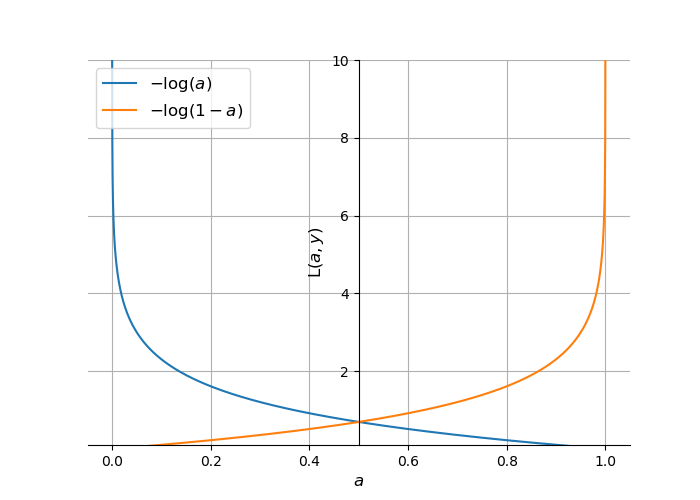
\includegraphics[scale=0.9]{png/loss.png} 
\caption{Loss function for $y=0$ and $y=1$}
\label{fig:loss}
\end{figure}
Next we define the overall loss function on the entire training set, i.e. on $m$ multiple samples. Assuming that the training examples are independent and identically distributed, then 
\[ P(Y=y) = \prod_{i=1}^{m} P(y^{(i)}|\bm{x}^{(i)})
\]
From equation \eqref{eqn:joint}, we would want to maximize 
\[
\prod_{i=1}^{m} a^{(i)^{y^{(i)}}} \cdot\left(1-a^{(i)}\right)^{\left(1-y^{(i)}\right)}
\]
over $\bm{w}$ and $b$  for multiple samples, which is equal to 
\[ \begin{split}
{\argmax_{\textbf{w},b} \log \left(\prod_{i=1}^{m} a^{(i)^{y^{(i)}}} \cdot\left(1-a^{(i)}\right)^{\left(1-y^{(i)}\right)}\right)} &=\argmax_{\textbf{w},b} \sum_{i=1}^{m} \log \left(a^{(i)^{y^{(i)}}} \cdot\left(1-a^{(i)}\right)^{\left(1-y^{(i)}\right)}\right) \\
  &=\argmax_{\textbf{w},b} \sum_{i=1}^{m} y^{(i)} \log \left(a^{(i)}\right)+\left(1-y^{(i)}\right) \log \left(1-a^{(i)}\right)
\end{split} \]
or, equivalently, we want to minimize 
\begin{equation}\label{eqn:cost}
\begin{split}
\mathrm{J}(\bm{w}, b) &=-\frac{1}{m} \sum_{i=1}^{m}\left[\left(y^{(i)} \log \left(a^{(i)}\right)+\left(1-y^{(i)}\right) \log \left(1-a^{(i)}\right)\right]\right. \\
	&=\frac{1}{m} \sum_{i=1}^{m} \mathrm{L}\left(a^{(i)}, y^{(i)}\right)
\end{split}
\end{equation}
Equation \eqref{eqn:cost} is called the {cost function} which measures how well parameters $\bm{w}$ and $b$ are doing on the entire training set $(\bm{X},\bm{y})$. It would be required to show that $\mathrm{J}(\bm{w},b)$ given in equation \eqref{eqn:cost} is a convex function which guarantees a local minimum, which is a global minimum (from Theorem \ref{thm:local_is_global}) for the function. 
\begin{equation}
\begin{split}
\frac{\partial \mathrm{L}}{\partial a} &=
   \frac{\partial}{\partial a} \left ( - \left( y \text{log}(a) + (1-y)\text{log}(1-a)\right) \right ) \\ 
   &= \frac{\partial}{\partial a} \left ( - y \text{log} (a) \right ) +  \frac{\partial}{\partial a} \left (- (1-y)\text{log}(1-a) \right ) \\
   &=\frac{-y}{a} + \frac{1-y}{1-a} = \frac{a-y}{a(1-a)}
\end{split}
\end{equation}
From equation \eqref{eqn:sigma2}, 
\[ \frac{da}{dz} = a(1-a) \]
Using chain rule;
\begin{equation}\label{eqn:dldz}
\frac{\partial \mathrm{L}}{\partial z} = \frac{\partial \text{L}}{\partial a} \frac{d a}{d z} = \frac{a-y}{a(1-a)}a(1-a) = a-y  
\end{equation}
\[ \frac{\partial \mathrm{L}}{\partial \bm{w}} =
   \frac{\partial \mathrm{L}}{d z} \frac{\partial z}{\partial \bm{w}} = (a - y)\bm{x}, \quad
   \frac{\partial \text{L}}{\partial b} =
   \frac{\partial \text{L}}{\partial z} \frac{\partial z}{\partial b} = (a - y)
\]
Hence 
\begin{equation}\label{eqn:djdz}
\frac{\partial \mathrm{J}}{\partial \bm{w}} = \frac{1}{m}\sum_{i=1}^{m} (a^{(i)} - y^{(i)})\bm{x}^{(i)}, \quad \frac{\partial \mathrm{J}}{\partial b} = \frac{1}{m}\sum_{i=1}^{m} (a^{(i)} - y^{(i)})
\end{equation}

If it can be proved that the functions $-\log a$ and $-\log (1-a)$ are convex functions of $\bm{w}$ and $b$, then the objective function 
\[ \mathrm{J}(\bm{w}, b) = -\frac{1}{m} \sum_{i=1}^{m}\left[\left(y^{(i)} \log \left(a^{(i)}\right)+\left(1-y^{(i)}\right) \log \left(1-a^{(i)}\right)\right]\right.
\]
must also be convex since any linear combination of two or more convex functions is also convex (Lemma \ref{lemma:sum}). Using the second order condition from Theorem \ref{thm:second_order}.  Deriving the Hessian of $-\log(a)$ with respect to $\bm{w}$
\begin{equation}\label{eqn:hess_w_1}
\begin{split}
\nabla^2_{\bm{w}}[-\log (a)] &= \nabla_{\bm{w}}\{\nabla_{\bm{w}}[-\log (a)]\} = \nabla_{\bm{w}}\left\{\frac{d(-\log (a))}{da}.\frac{da}{dz}.\frac{\partial z}{\partial \bm{w}} \right\} \\
	&=\nabla_{\bm{w}}\left\{ -\frac{1}{a}.[a(1-a)].\bm{x} \right\} = \nabla_{\bm{w}}\left\{ (a-1).\bm{x} \right\} \\
	&= \frac{d((a-1).\bm{x})}{da}.\frac{da}{dz}.\frac{\partial z}{\partial \bm{w}} = \bm{x}.[a(1-a)].\bm{x} \\
\nabla^2_{\bm{w}}[-\log (a)] &= a(1-a)\bm{x}\bm{x}^T	
\end{split}
\end{equation}
Similarly, for the Hessian of $-\log(a)$ with respect to $b$ 
\begin{equation}\label{eqn:hess_b_1}
\begin{split}
\nabla^2_b[-\log (a)] &= \nabla_b\{\nabla_b[-\log (a)]\} = \nabla_b\left\{\frac{d(-\log (a))}{da}.\frac{da}{dz}.\frac{\partial z}{\partial b} \right\} \\
	&=\nabla_b\left\{ -\frac{1}{a}.[a(1-a)] \right\} = \nabla_b\left\{ (a-1) \right\} \\
	&= \frac{d((a-1))}{da}.\frac{da}{dz}.\frac{\partial z}{\partial \bm{w}} = a(1-a) \\
\nabla^2_b[-\log (a)] &= a(1-a)	
\end{split}
\end{equation}
To show that the Hessian matrices in equation \ref{eqn:hess_w_1} and \ref{eqn:hess_b_1} are positive semi-definite
\begin{equation}\label{eqn:positive1}
\begin{split}
\forall \; \bm{q}\in \mathbb{R}^n: \;\; \bm{q}^T \nabla_{\bm{w}}^2[-\log(a)] \bm{q} & =  \bm{q}^T \left[ a(1-a)\bm{x}\bm{x}^T \right] \bm{q} \\ 
& =  a (1 - a) (\bm{x}^T \bm{q})^2 \geq 0 
\end{split}
\end{equation}
\begin{equation}\label{eqn:positive2}
\begin{split}
\forall \; \bm{q}\in \mathbb{R}^n: \;\; \bm{q}^T \nabla_{\bm{w}}^2[-\log(a)] \bm{q} & =  \bm{q}^T \left[ a(1-a)\bm{x}\bm{x}^T \right] \bm{q} \\ 
& =  a (1 - a) (\bm{x}^T \bm{q})^2 \geq 0 
\end{split}
\end{equation}
Deriving the Hessian of $-\log(1-a)$ with respect to $\bm{w}$
\begin{equation}\label{eqn:hess_w_2}
\begin{split}
\nabla^2_{\bm{w}}[-\log (1-a)] &= \nabla_{\bm{w}}\{\nabla_{\bm{w}}[-\log (1-a)]\} = \nabla_{\bm{w}}\left\{\frac{d(-\log (1-a))}{da}.\frac{da}{dz}.\frac{\partial z}{\partial \bm{w}} \right\} \\
	&=\nabla_{\bm{w}}\left\{ -\frac{1}{1-a}.[a(1-a)].\bm{x} \right\} = \nabla_{\bm{w}}\left\{ -a\bm{x} \right\} \\
	&= \frac{d(-a\bm{x})}{da}.\frac{da}{dz}.\frac{\partial z}{\partial \bm{w}} = \bm{x}.[a(1-a)].\bm{x} \\
\nabla^2_{\bm{w}}[-\log (a)] &= a(1-a)\bm{x}\bm{x}^T	
\end{split}
\end{equation}
Similarly, for the Hessian of $-\log(1-a)$ with respect to $b$ 
\begin{equation}\label{eqn:hess_b_2}
\begin{split}
\nabla^2_b[-\log (1-a)] &= \nabla_b\{\nabla_b[-\log (1-a)]\} = \nabla_b\left\{\frac{d(-\log (1-a))}{da}.\frac{da}{dz}.\frac{\partial z}{\partial b} \right\} \\
	&=\nabla_b\left\{ -\frac{1}{1-a}.[a(1-a)] \right\} = \nabla_b\left\{ -a \right\} \\
	&= \frac{d(-a)}{da}.\frac{da}{dz}.\frac{\partial z}{\partial \bm{w}} = a(1-a) \\
\nabla^2_b[-\log (a)] &= a(1-a)	
\end{split}
\end{equation}
It has been shown that equations \eqref{eqn:hess_w_2} and \eqref{eqn:hess_b_2} are positive semi-definite in equations \eqref{eqn:positive1} and \eqref{eqn:positive2} respectively. Hence the cost function $\mathrm{J}(\bm{w},b)$ given in \eqref{eqn:cost} is convex which guarantees a global minimum for the function.

\section{Gradient Descent}\label{sec:gd}
Gradient-based learning procedures have been used since the late 1950's but they were mostly limited to linear systems {\cite{dudaHart1973}}. The surprising usefulness of such simple gradient descent techniques for complex machine learning tasks was not widely realized until it was realised that:
\begin{itemize}[label = -]
\item The presence of a local minima for the loss function was not a major problem in practice. In fact, the local minima was not an hindrance to the  success of early non-linear gradient-based learning techniques such as Boltzmann machines {\cite{ahs-labm-85}}.
\item The efficiency of the back-propagation algorithm to compute the gradient in a non-linear system composed of several layers of processing.
\item The demonstration that the back-propagation procedure applied to multi layer neural networks with sigmoidal units can solve complicated learning tasks.
\end{itemize}
To find the parameters $\bm{w},\;b$ that minimizes the cost function $\mathrm{J}(\bm{w},\;b)$, we use the gradient descent algorithm; which is an optimisation algorithm used to minimize some function by iteratively moving in the direction of steepest descent as defined by the negative of the gradient. It involves the following steps:
\begin{enumerate}
\item Initialize parameters $\bm{w},\; b$ to some initial value, and calculate $\mathrm{J}(\bm{w},\;b)$. We can initialize to zeros or any random number, initializing to zeros is preferable for logistic regression. The same global minimum point would be reached regardless of initial point since the cost function is convex. 
\item Take a step in steepest downhill direction using the negative gradient with respect to $\bm{w}, \; b$. The size of these steps is called the learning rate, $\alpha$. With a high learning rate we can cover more ground each step, but we risk overshooting the lowest point since the slope of the function is constantly changing. With a very low learning rate, we can confidently move in the direction of the negative gradient since we are recalculating it so frequently, a low learning rate is more precise. 
\item Update the parameters with the gradients to reach the optimal values where $\mathrm{J}(\bm{w},\;b)$ is minimized.
\item Repeat steps 2 and 3 till further adjustments to parameters does not significantly reduce $\mathrm{J}(\bm{w},\;b)$.
\end{enumerate}
The steps above can be summarised as;
\[\begin{array}{rc}
\text{ Repeat until convergence} & \{  \\ 
 & \\
\bm{w}  :=  \bm{w} - \alpha \dfrac{\partial \mathrm{J}(\bm{w},\;b)}{\partial \bm{w}} & \\ \\
b  :=  b - \alpha \dfrac{\partial \mathrm{J}(\bm{w},\;b)}{\partial b} \\
& \}  
\end{array}\]
Theoretically, considering the problem:
\[
\bm{x}^{*}=\arg \min _{\bm{x} \in \mathbb{R}^{m}} f(\bm{x})
\]
choosing a suitable learning rate $\alpha > 0$, gradient descent is an iterative method;
\begin{equation}\label{eqn:gd}
\bm{x}^{k+1} = \bm{x}^k - \alpha \nabla f(\bm{x}^k)
\end{equation}
where $f:\mathbb{R}^m \rightarrow \mathbb{R}$ is the objective function to be minimised, and $\bm{x} \in \mathbb{R}^m$. Next, we analyse the convergence rate of the gradient descent algorithm. 

\begin{thm}\label{thm:gd_converge}
\normalfont {\cite{bottou2018optimization}}
Suppose the function $f: \mathbb{R}^{m} \rightarrow \mathbb{R}$ is convex and twice continuously differentiable, and it is L-smooth (i.e. its gradient is Lipschitz continuous with constant $L>0$): 
\begin{equation}\label{eqn:lipschitz}
\|\nabla f(\bm{x})-\nabla f(\bm{y})\|_{2} \leq L\|\bm{x}-\bm{y}\|_{2}
\end{equation}
for any $\bm{x}, \bm{y}\in \mathbb{R}^m$. Gradient descent for $k$ iterations with  fixed learning rate $\alpha \leq 1 / L$  satisfies
\begin{equation}\label{eqn:sublinear_conv}
f\left(\bm{x}^{(k)}\right)-f\left(\bm{x}^{*}\right) \leq \frac{\left\|\bm{x}^{(0)}-\bm{x}^{*}\right\|_{2}^{2}}{2 \alpha k}
\end{equation}
where $f\left(\bm{x}^{*}\right)$ is the optimal value of $f(\bm{x})$. \\ Intuitively, this means that gradient descent converges sublinearly with rate $\mathcal{O}(1 / k)$. %in order to achieve a bound of $f\left(\bm{x}^{(k)}\right)-f\left(\bm{x}^{*}\right) \leq \epsilon$, we must run $\mathcal{O}(1/ \epsilon)$ iterations of gradient descent.
\end{thm}

\begin{proof}
If $f$ is twice differentiable, then we have by Taylor first order expansion 
\[
\nabla f(\bm{x}+\alpha \bm{d})=\nabla f(\bm{x})+\int_{0}^{\alpha} \nabla^{2} f(\bm{x}+t \bm{d}) \bm{d}\;\mathrm{d}t
\]
\[
\Longrightarrow \nabla f(\bm{x}+\alpha \bm{d})-\nabla f(\bm{x})=\int_{0}^{\alpha} \nabla^{2} f(\bm{x}+t \bm{d}) \bm{d}\;\mathrm{d}t
\]
where $\bm{d} \in \mathbb{R}^m$, $t\in(0,\alpha)$, taking norm of both sides we get
\[
\left\|\int_{0}^{\alpha} \nabla^{2} f(\bm{x}+t \bm{d}) \bm{d}\;\mathrm{d}t\right\|_{2} \leq L \alpha\|\bm{d}\|_{2}
\]
dividing through by $\alpha\|\bm{d}\|$, $\bm{d}\neq 0$ 
\[
\frac{\left\|\int_{0}^{\alpha} \nabla^{2} f(\bm{x}+t \bm{d}) \bm{d} \;\mathrm{d}t\right\|_{2}}{\alpha\|\bm{d}\|_2} \leq L \Longrightarrow \frac{\left\|\alpha \nabla^{2} f(\bm{x}) \bm{d}\right\|_{2}}{\alpha\|\bm{d}\|_2}+O(\alpha) \leq L
\]
taking limit as $\alpha \rightarrow 0$, we get 
\[
= \frac{\left\|\alpha \nabla^{2} f(\bm{x}) \bm{d}\right\|_{2}}{\bm{d}} \leq L, \quad \forall \;\bm{d} \neq 0 \in \mathbb{R}^{m}
\]
Taking the supremum over $\bm{d} \neq 0 \in \mathbb{R}^{m}$ in the above gives
\begin{equation}
\nabla^{2} f(\bm{x}) \preceq L I
\end{equation}
%Our assumption that $\nabla f$ is Lipschitz continuous with constant $L$,  implies that \\ $\nabla^{2} f(\bm{x}) \preceq L I$, 
or equivalently that $\nabla^{2} f(\bm{x})-L I$ is a negative semi-definite matrix. Hence, 
\begin{equation}\label{eqn:a}
(\bm{x} - \bm{y})^T (\nabla^{2} f(\bm{x})-L I) (\bm{x} - \bm{y}) \leq 0
\end{equation}
where the LHS of \eqref{eqn:a} is the quadratic form of $\nabla^{2} f(\bm{x})-L I$.

\noindent Since $L>0$, and using the non-negativity property of norm, we have that
\begin{equation}\label{eqn:b}
L\|\bm{x}-\bm{y}\|_2^2 \geq 0
\end{equation}
Combining equations \eqref{eqn:a} and \eqref{eqn:b}, we get 
\begin{equation}\label{eqn:c}
L\|\bm{x}-\bm{y}\|_2^2 \geq (\bm{x} - \bm{y})^T \nabla^{2} f(\bm{x}) (\bm{x} - \bm{y})
\end{equation}
Performing a quadratic expansion of $f$ around $f(x)$; 
\begin{equation*}
\begin{split}
f(\bm{y}) & = f(\bm{x})+\nabla f(\bm{x})^{T}(\bm{y}-\bm{x})+\frac{1}{2} (\bm{y}-\bm{x})^T \nabla^{2} f(\bm{x}) (\bm{y}-\bm{x}) \\
& \leq f(\bm{x})+\nabla f(\bm{x})^{T}(\bm{y}-\bm{x})+\frac{1}{2} L\|\bm{y}-\bm{x}\|_{2}^{2} \qquad\qquad \text{from \eqref{eqn:c}}
\end{split}
\end{equation*}
Plugging in  gradient descent update by letting $y=\bm{x}^{+}=\bm{x}- \alpha \nabla f(\bm{x})$, we get:
\begin{equation}\label{eqn:d}
\begin{split}
f(\bm{x}^{+}) & \leq f(\bm{x})+\nabla f(\bm{x})^{T}\left(\bm{x}^{+}-\bm{x}\right)+\frac{1}{2} L\left\|\bm{x}^{+}-\bm{x}\right\|_{2}^{2} \\
&=f(\bm{x})+\nabla f(\bm{x})^{T}(\bm{x}-\alpha\nabla f(\bm{x})-\bm{x})+\frac{1}{2} L\|\bm{x}- \alpha \nabla f(\bm{x})-\bm{x}\|_{2}^{2} \\
&=f(\bm{x})-\nabla f(\bm{x})^{T} \alpha \nabla f(\bm{x})+\frac{1}{2} L\|\alpha \nabla f(\bm{x})\|_{2}^{2} \\
&=f(\bm{x})-\alpha\|\nabla f(\bm{x})\|_{2}^{2}+\frac{1}{2} L^{2}\|\nabla f(\bm{x})\|_{2}^{2} \\
f(\bm{x}^{+}) &=f(\bm{x})-\left(1-\frac{1}{2} L \alpha\right) \alpha\|\nabla f(\bm{x})\|_{2}^{2}
\end{split}
\end{equation}
Using $\alpha \leq 1 / L$,  $-\left(1-\frac{1}{2} L \alpha\right)=\frac{1}{2} L \alpha-1 \leq \frac{1}{2} L\left(\frac{1}{L}\right)-1=-\frac{1}{2}$. Substituting this result into \eqref{eqn:d} we get:
\begin{equation}\label{eqn:e}
f\left(\bm{x}^{+}\right) \leq f(\bm{x})-\frac{1}{2} \alpha\|\nabla f(\bm{x})\|_{2}^{2}
\end{equation}
since $\frac{1}{2} \alpha\|\nabla f(\bm{x})\|_{2}^{2}$ will always be positive unless $\nabla f(\bm{x})=0,$ this inequality implies that the objective function value strictly decreases with each iteration of gradient descent until it reaches the optimal value $f(\bm{x})=f\left(\bm{x}x^{*}\right)$. But this convergence result only holds when we choose the learning rate $\alpha$ to be small enough, i.e. $\alpha \leq \frac{1}{L}$. 

\noindent Next, we bound $f\left(\bm{x}^{+}\right),$ the objective value at the next iteration, in terms of $f\left(\bm{x}^{*}\right),$ the optimal objective value. Since $f$ is convex, 
\begin{equation}\label{eqn:f}
\begin{split}
f(\bm{x}^{*}) &\geq f(\bm{x})+\nabla f(\bm{x})^{T}(\bm{x}^{*}-\bm{x}) \\
\Longrightarrow f(\bm{x}) &\leq f(\bm{x}^{*})+\nabla f(\bm{x})^{T}(\bm{x}-\bm{x}^{*})
\end{split}
\end{equation}
Plugging this into \eqref{eqn:e} we obtain:
\begin{equation}\label{eqn:g}
\begin{split}
f(\bm{x}^{+})  & \leq f(\bm{x}^{*})+\nabla f(\bm{x})^{T}(\bm{x}-\bm{x}^{*})- \frac{\alpha}{2}\|\nabla f(\bm{x})\|_{2}^{2} \\
\Longrightarrow f(\bm{x}^{+})-f(\bm{x}^{*}) & \leq \frac{1}{2 \alpha}\left[\; 2 \alpha \nabla f(\bm{x})^{T}(\bm{x}-\bm{x}^{*})-\alpha^{2}\|\nabla f(\bm{x})\|_{2}^{2}\;\right] \\
\Longrightarrow f(\bm{x}^{+})-f(\bm{x}^{*}) & \leq \frac{1}{2 \alpha}\left[\; 2 \alpha \nabla f(\bm{x})^{T}(\bm{x}-\bm{x}^{*})-\alpha^{2}\|\nabla f(\bm{x})\|_{2}^{2}-\|\bm{x}-\bm{x}^{*}\|_{2}^{2}+\|\bm{x}-\bm{x}^{*}\|_{2}^{2}\;\right] \\
\Longrightarrow f(\bm{x}^{+})-f(\bm{x}^{*}) & \leq \frac{1}{2 \alpha}\left[\; \|\bm{x}-\bm{x}^{*}\|_{2}^{2}-\|\bm{x}-\alpha \nabla f(\bm{x})-\bm{x}^{*}\|_{2}^{2}\;\right] 
\end{split}
\end{equation}
Substituting a gradient descent update $\bm{x}^{+}=\bm{x}-\alpha \nabla f(\bm{x})$ in \eqref{eqn:g}, we get:
\begin{equation}
f\left(\bm{x}^{+}\right)-f\left(\bm{x}^{*}\right) \leq \frac{1}{2 \alpha}\left(\left\|\bm{x}-\bm{x}^{*}\right\|_{2}^{2}-\left\|\bm{x}^{+}-\bm{x}^{*}\right\|_{2}^{2}\right)
\end{equation}
This inequality holds for $\bm{x}^{+}$ on every iteration of gradient descent. Summing over iterations, we get:
\begin{equation}
\begin{split}
\sum_{i=1}^{k} f(\bm{x}^{(i)})- f(\bm{x}^{*}) & \leq \sum_{i=1}^{k} \frac{1}{2 \alpha}\left(\left\|\bm{x}^{(i-1)}-\bm{x}^{*}\right\|_{2}^{2}-\left\|\bm{x}^{(i)}-\bm{x}^{*}\right\|_{2}^{2}\right) \\
&=\frac{1}{2 \alpha}\left(\left\|\bm{x}^{(0)}-\bm{x}^{*}\right\|_{2}^{2}-\left\|\bm{x}^{(k)}-\bm{x}^{*}\right\|_{2}^{2}\right) \\
& \leq \frac{1}{2 \alpha}\left(\left\|\bm{x}^{(0)}-\bm{x}^{*}\right\|_{2}^{2}\right)
\end{split}
\end{equation}
where the summation on the right-hand side disappears because each subsequent terms cancel each other, leaving only the initial and final terms. Finally, using the fact that $f$ decreases on every iteration, we can conclude that
\begin{equation}
\begin{split}
f\left(\bm{x}^{(k)}\right)-f\left(\bm{x}^{*}\right) & \leq \frac{1}{k} \sum_{i=1}^{k} f\left(\bm{x}^{(i)}\right)-f\left(\bm{x}^{*}\right) \\
& \leq \frac{\left\|\bm{x}^{(0)}-\bm{x}^{*}\right\|_{2}^{2}}{2 \alpha k}
\end{split}
\end{equation}
which gives the inequality \eqref{eqn:sublinear_conv}.
\end{proof}
\begin{thm}
\normalfont {\cite{bottou2018optimization}}
Suppose the function $f: \mathbb{R}^{m} \rightarrow \mathbb{R}$ is $\mu$-strongly convex and $L$-smooth. Gradient descent for $k$ iterations with  fixed learning rate $\alpha \leq 2 / (\mu + L)$ satisfies
\begin{equation}\label{eqn:linear_conv}
f\left(\bm{x}^{(k)}\right)-f\left(\bm{x}^{*}\right) \leq c^k \frac{L}{2} \left\|\bm{x}^{(0)}-\bm{x}^{*}\right\|_{2}^{2}
\end{equation}
where $0<c<1$ and $\mu > 0$. \\ 
This means that gradient descent on a strong convex function converges linearly with rate $\mathcal{O}(c^k)$ which is a faster convergence rate than that of convex functions. %and in order to achieve a bound of $f\left(\bm{x}^{(k)}\right)-f\left(\bm{x}^{*}\right) \leq \epsilon$, we must run $\mathcal{O}(\log(1/ \epsilon))$ iterations of gradient descent.
\end{thm}
\noindent One of the key problems in gradient descent is that we might overshoot the optimal value or make insufficient progress. A simple fix for the problem is to use line search in conjunction with gradient descent. That is, we use the direction given by $\nabla f(\bm{x})$ and then perform binary search as to which learning rate $\alpha$ minimizes $f(\bm{x} - \alpha\nabla f(\bm{x}))$.
This algorithm converges rapidly ({\cite{boyd2004convex}}). However, for the purpose of deep learning this is not quite so feasible, since each step of the line search would require us to evaluate the objective function on the entire dataset. This is way too costly to accomplish.

\section{Stochastic Gradient Descent}\label{sec:sgd}
In deep learning, the objective (cost) function is usually the average of the loss functions for each example in the training dataset. Assuming that $f_i(\bm{x})$ is the loss function of the training data instance with $m$ examples, an index of $i$, and parameter vector of $\bm{x}$, then we have the objective function:
\begin{equation}\label{eqn:sgd_obj}
f(\bm{x}) = \frac{1}{m}\sum_{i=1}^m f_i(\bm{x})
\end{equation}
The gradient of the objective function at $\bm{x}$ is computed as
\[
\nabla f(\bm{x})=\frac{1}{m} \sum_{i=1}^{m} \nabla f_{i}(\bm{x})
\]
gradient descent would repeat:
\[
\bm{x}^{k+1} = \bm{x}^k - \alpha \nabla f(\bm{x}^k)
\]
if gradient descent is used, the computing cost for each independent variable iteration is $\mathcal{O}(n)$ which grows linearly with $n$. Therefore, when the model training data instance is large, the cost of gradient descent for each iteration will be very high.

Stochastic gradient descent (SGD) {\cite{robbins1951stochastic}} is ideal in the context of large scale machine learning, it reduces computational cost at each iteration by uniform sampling an index $i_k \in\{1, \ldots, m\}$ for data instances at random, and compute the gradient $\nabla f_{i_{k}}(\bm{x})$ to update $\bm{x}$:
\begin{equation}\label{eqn:sgd}
\bm{x}^{k+1}=\bm{x}^{k}- \alpha_k \cdot \nabla f_{i_{k}}\left(\bm{x}^{k}\right), \quad k=1,2,3, \ldots
\end{equation}
where $i_{k} \in\{1, \ldots, m\}$ is some chosen index at iteration $k$ and $\alpha_k$ is the learning rate at iteration $k$. The computing cost for each iteration drops from $\mathcal{O}(n)$ of the gradient descent to the constant $\mathcal{O}(1)$. Stochastic gradient descent uses an unbiased estimate of the gradient $\nabla f(\bm{x})$ at each step, i.e,
\begin{equation}\label{eqn:sgd_est}
\mathbb{E}[\nabla f_{i_{k}}(\bm{x})]=\frac{1}{m} \sum_{i=1}^{m} \nabla f_{i}(\bm{x})  = \nabla f(\bm{x})
\end{equation}
The iterate sequence is not determined uniquely by the function $f$, the starting point $\bm{x}^1$, and the sequence of step sizes $\{\alpha_k\}$, as it would in gradient descent. Rather, $\{\bm{x}_k\}$ is a stochastic process whose behaviour is determined by the random sequence $\{i_k\}$.
\begin{thm}
\normalfont {\cite{nemirovski2009robust}}
Suppose $f:\mathbb{R}^m\rightarrow\mathbb{R}$ is convex, stochastic gradient descent with diminishing learning rate $\alpha_k = 1/k$ satisfies
\[
\mathbb{E}[f(\bm{x}^{(k)})] - f(\bm{x}^*) = \mathcal{O}(1/\sqrt{k})
\]
When $f$ is $\mu$-strongly convex and L-smooth, stochastic gradient descent with diminishing learning rate $\alpha_k = \theta/k$, with constant $\theta > 1/(2\mu)$ satisfies
\[
\mathbb{E}[f(\bm{x}^{(k)})] - f(\bm{x}^*) = \mathcal{O}(1/k)
\]
\end{thm}
\noindent
This shows that stochastic gradient descent does not enjoy the linear convergence rate of gradient descent under strong convexity.

A popular method used in deep learning is to 
%A compromise between computing the true gradient and the gradient at a single example is to 
compute the gradient against more than one training example, called a minibatch, at each step. This method improves computational efficiency compared to stochastic gradient descent, because the code can make use of vectorization libraries rather than computing each step separately. It may also result in smoother convergence, as the gradient computed at each step is averaged over more training examples. 

In minibatch stochastic gradient descent,  we choose a random subset $I_{k} \subseteq\{1, \ldots, m\},\;\left|I_{k}\right|=b \ll m,$ repeat:
\begin{equation}\label{eqn:mini_sgd}
\bm{x}^{k+1}=\bm{x}^{k}- \alpha_k \cdot \frac{1}{b} \sum_{i \in I_{k}} \nabla f_{i}\left(\bm{x}^{k}\right), \quad k=1,2,3, \ldots
\end{equation}
Again, we are approximating full gradient by an unbiased estimate
\[
\mathbb{E}\left[\frac{1}{b} \sum_{i \in I_{k}} \nabla f_{i}(\bm{x})\right]=\nabla f(\bm{x})
\]
% Using mini-batches reduces variance by a factor $1 / b,$ but is also $b$ times more expensive. 
\begin{thm}
\normalfont {\cite{dekel2012optimal}} 
Let $f:\mathbb{R}^m\rightarrow\mathbb{R}$ be an $L$-smooth convex function and assume that the stochastic gradient $\nabla f_i(\bm{x}^k)$ has $\sigma^2$-bounded variance for all $\bm{x} \in \mathbb{R}^n$, i.e.
\[
\mathbb{E}\left[\;\|\nabla f(\bm{x}) - \nabla\mathbb{E}\{f(\bm{x})\} \|_2\;\right] \leq \sigma^2
\]
then the convergence rate of minibatch stochastic gradient descent, with minibatch size $b$ after $k$ iterations is of order $\mathcal{O}(1/\sqrt{bk}+1/k)$.
\end{thm}
\noindent
Since the total number of examples examined is $bk$ though there is only an increase of $\sqrt{b}$ times, the convergence speed degrades with increasing minibatch size $b$.

\section{Regularisation}\label{sec:regularisation}
The fundamental problem of machine learning is the conflict between optimisation and generalisation. Optimisation refers to the process of modifying a model parameters to produce the best possible outcome on the training data, whereas generalisation refers to how well the trained model performs on data it has never seen before. The goal is to achieve good generalisation, but generalisation can not be monitored; the model can only changed based on its training data. 

Optimisation and generalisation are associated at the beginning of the training: the lower the loss on the training data, the lower the loss on test results. The model is said to be {underfit} as this is happening, there is still progress to be made because the network has not yet modelled all the related trends in the training data. But after a number of iterations on the training data, generalisation will stop improving and validation metrics will stop and then start degrading; the model will start to {overfit}. That is, trends which are common to training data but which are deceptive or meaningless when it comes to new data are beginning to be learned.

To prevent a model from overfitting, the best solution is to get more training data; a model trained on more data will naturally generalise better. If that is not feasible, the next best solution is by regularisation, i.e., to modulate the amount of information the model can store or impose limits on what information the model can store. If only a small number of patterns can be memorized by a network, the optimisation process would cause it to concentrate on the most prominent patterns, which have a better chance of generalising well.
\begin{figure}[htb]
\centering
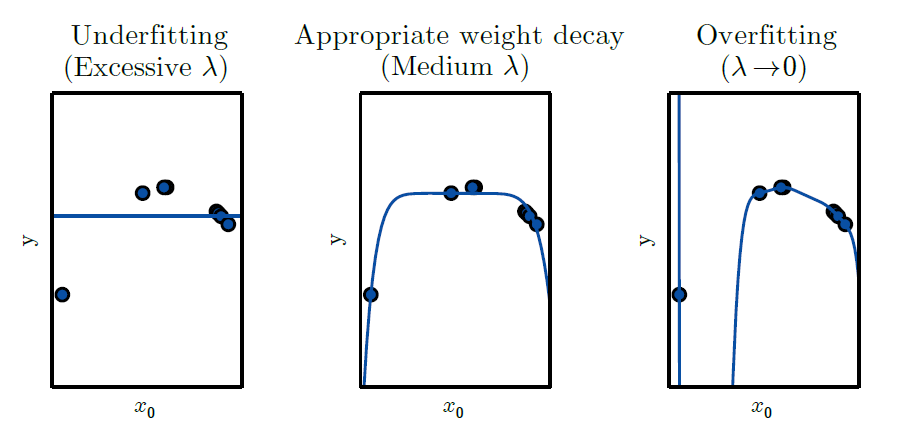
\includegraphics[scale=0.8]{png/lambda.png} 
\caption[Regularisation constant effect on underfitting and overfitting in a model]{Regularisation constant effect on underfitting and overfitting in a model, \protect{\cite{10.5555/3086952}}}
\label{fig:lambda}
\end{figure}

Modulating the amount of information the model can store is done by reducing  the number of learnable parameters in the model. A model with more parameters has more memorizing ability and can therefore easily learn a perfect dictionary-like mapping between the training samples and their targets — a mapping without generalizing strength. Imposing limits on what information the model can store is achieved by {weight regularisation}; in which complexity of a model is constrained by forcing its weights to take only small values, which makes the distribution of weight values more {regular}. Weight regularization is done by adding to the cost function of the model a cost associated with having large weights. The cost comes in two forms
\begin{itemize}
\item $L^1$ regularisation: The cost added is the $L^1$ norm of the weights.
\item $L^2$ regularisation: The cost added is the square $L^2$ norm of the weights, it is the most widely used technique for regularising machine learning models. Hence, the new objective function for a logistic regression model with $L^2$ regularisation would be;
\begin{equation}\label{eqn:cost_regularisation}
\mathrm{J}(\bm{w}, b) =-\frac{1}{m} \sum_{i=1}^{m}\left[\left(y^{(i)} \log \left(a^{(i)}\right)+\left(1-y^{(i)}\right) \log \left(1-a^{(i)}\right)\right]\right. + \frac{\lambda}{2}\|\bm{w}\|_2^2
\end{equation}
where $\lambda\geq 0$ is an hyperparameter called the {regularisation constant}, and it governs the amount of regularisation. For $\lambda = 0$, the  original cost function is recovered, whereas for $\lambda > 0$ we ensure that $\bm{w}$ cannot grow too large. $L^2$ regularisation is also called weight decay in the context of neural networks. 
\end{itemize}
Since the square $L^2$ norm of weights $\frac{\lambda}{2}\|\bm{w}\|_2^2$ is a strongly convex function (it has a quadratic lower bound at every chosen point), the cost function $\mathrm{J}(\bm{w}, b)$ in \eqref{eqn:cost_regularisation} becomes a strongly convex function (Proposition \ref{pro:sum}), hence gradient descent applied on a $L^2$ regularised cost function converges faster.


\section{Decision Boundary}
The decision boundary is a function that separates the two classes, $y=0$ and $y=1$.  
\begin{figure}[H]
\centering
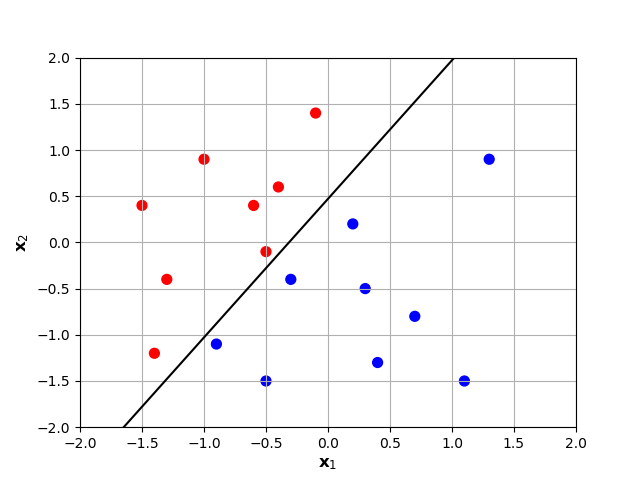
\includegraphics[scale=0.8]{png/boundary.png} 
\caption{Decision boundary for two inputs $\bm{x}_1$ and $\bm{x}_2$}
\label{fig:boundary}
\end{figure} 
\noindent
When $z=0$, then $\hat{y}=0.5$ due to the sigmoid function's $y$-intercept. The decision boundary is a hyperplane of the equation $\bm{w}^T\bm{x}=0$ as it discriminates the two different regions of classification. On the left hand side of the decision boundary where $z<0$, the output is $a<0.5$, thus class $0$ is predicted, while class $1$ is predicted on the right side of the line.  If the parameters $\bm{w}$ and $b$ are not optimal, then the separation would be inaccurate, this provides intuition into  optimising  the parameters for the classification task.  
%Thus, when $z=0$ we are at a turning point as we switch from discrete classification of $0$ to $1$.
%\newpage 



%\section{Multilayer Perceptron}
%\section{Deep Learning}

%\section{Convolutional Neural Networks (CNN)}
%In image classification, CNNs outperform traditional image processing methods in several applications. This general trend is also observed in the automatic identification of crop diseases. Some of the selected studies compared the performance obtained with CNNs to that of other methods. In all of these studies, the CNN results are better than the others. % The difference of accuracy ranged from $3%$ (Brahimi et al., 2017) to $28.89%$ (Liu B. et al., 2017). 













\chapter{Literature Review}
\setcounter{section}{-1}
\section{Introduction}
Machine learning is a powerful tool in applying modern science area for achieving the incredible success in taking place of tedious and complex manual processing. In different science area, deep learning models play different roles in significant applications. Our focus in this project are on the problems involving computer vision area, which takes most advantages from Convolutional Neural Networks (CNNs). In this chapter, we discuss briefly the history of deep learning and provide a literature survey of past works in the application of machine learning to some agricultural problems, particularly in the areas of weed management, pest control, crop disease detection, plant phenotyping, plant growth and yield prediction.

\section{Deep Learning}
\subsection{Perceptrons}
The idea of connecting units to local receptive fields on the input goes back to the perceptron in 1958 {\cite{Rosenblatt58theperceptron}}. The perceptron was intended to be a machine, rather than a program. This machine was designed for image recognition: it had an array of $400$ photocells, randomly connected to the ``neurons''. Weights were encoded in potentiometers, and weight updates during learning were performed by electric motors {\cite{10.5555/1162264}}. Although the perceptron initially seemed promising, the constraint that similar input patterns lead to similar outputs lead to an inability of the system to learn certain mappings from input to output, which proved that perceptrons could not be trained to recognise many classes of patterns. 

Single layer perceptrons are only capable of learning linearly separable patterns. {\cite{MinskyPapert:69}} showed that it was impossible for these classes of network to learn an exclusive or (XOR) problem illustrated in Table (\ref{tab:xor}) (a logical operation that outputs true only when inputs differ). They also pointed out that, if there is a layer of simple perceptron like hidden units, with which the original input pattern can be augmented, there is always a recoding (i.e., an internal representation) of the input patterns in the hidden units in which the similarity of the patterns among the hidden units can support any required mapping from the input to the output units. Thus, if we have the right connections
from the input units to a large enough set of hidden units, we can always find a representation that will perform any mapping from input to output through these hidden units.
\begin{table}
\centering
\begin{tabular}{cc}
\hline
Input Pattern & Output \\
\hline
00 & 0 \\
10 & 1 \\
101& 1 \\
111 & 0 \\
010 & 1 \\
\hline
\end{tabular}
\caption{XOR table}
\label{tab:xor}
\end{table}

The limitations of the perceptron caused the field of neural network research to stagnate for many years, before it was recognised that a feedforward neural network with two or more layers (also called a multilayer perceptron) had greater processing power than perceptrons with one layer. Also, the Minsky and Papert text was often miscited to note that the multi-layer perceptron could not solve the XOR problem. This caused a significant decline in interest and funding of neural network research. It took ten more years until neural network research experienced a resurgence in the 1980s. 

\subsection{Back Propagation}
Connectionist architectures; where large numbers of weighted connections of ``neuron-like'' processing elements, with weighted connections (which encodes the knowledge of the system) between elements, and with emphasis on learning internal representations rather than having them hand programmed, which were developed to result in systems that are: fast and resistant to damage, able to generalise from its inputs, and to learn efficiently for large-scale masses drew considerable attention in the early 80's because of their interesting learning abilities. Among the numerous learning algorithms that have been proposed for complex connectionist networks, Back-Propagation (BP) is probably the most widespread. Back propagation was proposed in {\cite{RumelhartHintonWilliams86}} but had been developed before by several independent groups in different contexts and for different purposes, such as; {\cite{Kelley:1960}} in the context of control theory, {\cite{BrysonHo69}} in the framework of optimal control and system identification, {\cite{Werbos:74}} proposed that it could be used for neural networks, {\cite{7fa6b6a5cde14bcfbd7ab3a8f19d0d56}} in the learning of the threshold for asymmetrical network. The error back-propagation presented by {\cite{RumelhartHintonWilliams86}} showed experimentally that the method can generate useful internal representations of incoming data in hidden layers of neural networks which was crucial in the learning phase of deep neural networks.

\subsection{Convolutional Neural Networks}
{\cite{Hubel:62}} found that cells in a cat and monkey visual cortex are responsible for detecting light in receptive fields, these visual cortexes contain neurons that individually respond to small regions of the visual field. The ``neocognitron'' was introduced by {\cite{fukushima:neocognitronbc}}. It was inspired by the above-mentioned work of Hubel and Wiesel. The neocognitron introduced the two basic types of layers in Convolutional Neural Networks (CNNs): convolutional layers, and downsampling layers. A convolutional layer contains units whose receptive fields cover a patch of the previous layer. The weight vector (the set of adaptive parameters) of such a unit is often called a filter. Units can share filters. Downsampling layers contain units whose receptive fields cover patches of previous convolutional layers. Such a unit typically computes the average of the activations of the units in its patch. This downsampling helps to correctly classify objects in visual scenes even when the objects are shifted. The neocognitron is the first CNN which requires units located at multiple network positions to have shared weights. 

The Time Delay Neural Network (TDNN) was introduced by {\cite{10.5555/108235.108263}} and was the first convolutional network, as it achieved shift invariance. It did so by utilizing weight sharing in combination with backpropagation training. Thus, while also using a pyramidal structure as in the neocognitron, it performed a global optimisation of the weights, instead of a local one. TDNNs are convolutional networks that share weights along the temporal dimension, they allow speech signals to be processed time-invariantly.

A system to recognize hand-written ZIP Code numbers {\cite{NIPS1988_107}}  involved convolutions in which the kernel coefficients had been laboriously hand designed. {\cite{LeCun:89}} used back-propagation to learn the convolution kernel coefficients directly from images of hand-written numbers. Learning was thus fully automatic, performed better than manual coefficient design, and was suited to a broader range of image recognition problems and image types. This approach became a foundation of modern computer vision. 

LeNet-5, a pioneering 7-level convolutional network {\cite{lecun-gradientbased-learning-applied-1998}} that classifies digits, was applied by several banks to recognize hand-written numbers on  cheques digitized in $32\times 32$ pixel images. The ability to process higher resolution images requires larger and more layers of convolutional neural networks, so this technique was constrained by the availability of computing resources. This constraint lead to mostly bad performance of neural network models applied in the real world. 


\subsection{Long Short Term Memory}
With conventional back propagation through time {\cite{Werbos:88gasmarket}}, error signals flowing backwards in time tend to either blow up or vanish; the temporal updates of the backpropagated error exponentially depends on the size of the weight {\cite{10.1162/neco.1997.9.8.1735}}. Long Short Term Memory (LSTM) {\cite{10.1162/neco.1997.9.8.1735}}, overcame the error back-flow problems by learning to bridge time intervals in excess of $1000$ steps even in noisy input data, without loss of short time lag capabilities. This is achieved by an efficient, gradient-based algorithm. LSTMs are effective at capturing long term temporal dependencies. LSTM achieved record results in natural language text compression, and unsegmented connected handwriting recognition {\cite{graves09}}. As of 2016, major technology companies including Google, Apple, and Microsoft were using LSTMs as fundamental components in new products.

\subsection{Advancements in Computing Power}
Although CNNs were invented in the 1980s, their breakthrough in the 2000s required fast implementations on Graphics Processing Units (GPUs). GPUs are extremely efficient at matrix multiplication, which basically forms the core of machine learning. The strength of GPU lies in data parallelization, which means that instead of relying on a single core, as CPUs did before, a GPU can have many small cores. A single GPU can have thousands of Arithmetic Logic Units (ALUs), each performing a parallel computation to return a higher throughput faster, thus running complex computations in a short span of time. This makes GPUs highly suitable for performing complex matrix multiplications in a short span of time.

{\cite{gpu2004}}  showed that standard neural networks can be greatly accelerated on GPUs, their implementation was $20$ times faster than an equivalent implementation on CPU. {\cite{chellapilla:inria-00112631}} described GPU-implementation of a CNN on character recognition problems, their implementation was $4$ times faster than an equivalent implementation on CPU. {\cite{10.1162/NECO_a_00052}} showed that deep standard neural networks with many layers can be quickly trained on GPU by supervised learning through  backpropagation, their network outperformed previous machine learning methods on the Modified National Institute of Standards and Technology (MNIST) database (a large database of handwritten digits) handwritten digits benchmark. {\cite{Ciresan12multi-columndeep}} significantly improved on the best performance in the literature for multiple image databases, including the MNIST database {\cite{LeCun:89}}, the NORB (New York University Object Recognition Benchmark) dataset  (contains stereo image pairs of 50 uniform-coloured toys under 36 azimuths, 9 elevations, and 6 lighting conditions, for a total of 194,400 individual images) {\cite{10.5555/1896300.1896315}}, the HWDB1.0 dataset (containing $3,866$ hand-written Chinese characters) {\cite{icdar2011Chinese}}, the CIFAR-10 (Canadian Institute For Advanced Research) dataset (containing $60000$ $32 \times 32$ labelled RGB images) {\cite{krizhevsky2009learning}}, and traffic signs (dataset of more than $50,000$ traffic sign images) {\cite{stallkamp:11}}, using backpropagated trained deep CNNs implemented on GPUs.

The Tensor Processing Unit (TPU), an application-specific integrated circuit (ASIC) designed to accelerate artificial intelligence applications was announced by Google in 2016, it was built specifically for neural network machine learning on the TensorFlow framework. TPUs were used in the AlphaGo versus Lee Sedol series of man-machine Go games, where AlphaGo defeated human champions in Go {\cite{Silver_2016}}. Third generation cloud TPUs pods can deliver up to 100 petaFLOPS (floating point operations per second) per pod. This makes TPUs perfect for both training and inferencing of deep learning models, since training the models requires millions of floating points calculations. In addition to accuracy and speed, the TPUs also offer a higher energy efficient than conventional processing chips, consuming much less watts and also reducing the heat generated, TPUs are also a lot cheaper than GPUs and they are easily available on the cloud.

\section{Deep Learning in Agriculture}
Deep learning constitutes a modern technique for highly performing image processing and data analysis with credible results.  As deep learning has been applied in various domains, it has also found its place in the applied agriculture-analysis and phenotyping realm. Majority of those applications are based on typical CNN architectures to perform supervised classification to solve complex problems.
\subsection{Plant Phenotyping and Yield Prediction}
{\cite{10.1007/978-3-319-67361-5_18}} developed a model by coupling deep convolutional neural networks (fast region-based convolutional network, {\cite{DBLP:journals/corr/Girshick15}} and fully convolutional network, {\cite{DBLP:journals/corr/LongSD14}}) trained on a GTX 970 GPU together to measure stalk count and stalk width of Sorghum plants. The pipeline developed accurately extracts both detected object regions and dense semantic segmentation for extracting both stalk counts and stalk width. A ground robot was used to deploy a high-resolution stereo camera to capture dense image data of experimental plots of Sorghum plants in South Carolina and Mexico. Their method yielded an R-squared correlation of $0.88$ for stalk count and a mean absolute error of $2.77$mm where average stalk width is $14.354$mm. 

{\cite{taghavi:18}} proposed a CNN-LSTM framework for plant classification of various genotypes, LSTMs were also used to study the growth of the plants and their dynamic behaviours as important discriminative phenotypes for accession classification. A dataset of time series image sequences of four accessions of {Arabidopsis}, captured in similar imaging conditions, were used to train the models. The CNN-LSTM framework yielded an average accuracy of $93\%$.

{\cite{oliveira2018scalable}} applied recurrent LSTM layers to forecast pre-season soybean and maize yields for Brazil and USA yield. Field sensors, satellites, and unmanned aerial vehicles (UAVs) were used to derive precipitation, soil properties and seasonal climate forecasting datasets. The model had a root mean square percentage error of $14.31\%$, $12.85\%$ and  $15.28\%$ for Brazil-soybean, US-soybean, and  US-maize yields respectively. 

{\cite{agronomy9120833}} designed a two-step approach using unsupervised  deep CNNs and regression analysis to classify corn hybrids as either tolerant or susceptible to drought stress, heat stress, and combined drought and heat stress. The dataset used was from the 2019 Syngenta crop challenge {\cite{syngenta}}, several large datasets that recorded the yield performances of $2,452$ corn hybrids planted in $1,560$ locations between 2008 and 2017. The results labelled $121$ hybrids as drought tolerant, $193$ as heat tolerant, and $29$ as tolerant to both stresses. The proposed approach and its classification results were recognized as one of the winners of the Syngenta Crop Challenge.

{\cite{rasmussen2019maize}} adopted two CNN based deep learning-based methods (Multi-Task Network Cascades (MNC) and Region-Based Fully Convolutional Networks (R-FCN)) trained on NVIDIA Titan XP GPU  for corn silage kernel processing, which is an important step in determining the quality of silage harvested from a forage harvester. The dataset contained $2,500$ annotated RGB colour images of harvested silage which were taken over three years. Average precision scores for the model where $66.9\%$ and $71.8\%$ for R-FCN and MNC respectively.

{\cite{zhang2019deep}} applied the RetinaNet deep learning model {\cite{lin2017focal}} with different backbones to the problem of pod-counting and  flower detection in soybean crop production. Seven videos of soybean flower crops were captured by a ground robot under canopy level conditions in the field. $4,233$ annotated images extracted from those videos was used as the dataset. The model performed with a high degree of accuracy, which the highest accuracy reaching up to $95\%$.

\subsection{Weed Management and Pest Control}
{\cite{chen2018automatic}} proposed a method for segmentation and counting of aphid nymphs using CNNs (U-Net). Digital images of {pakchoi} (Chinese cabbage) leaves at different stages of aphid infestation were obtained and a binary mask at the corresponding pixel level was annotated for each image manually, identifying each pixel as a aphid (white) or background (black). After segmentation, they simply counted the number of connected white components as the amount of aphid nymphs for each image. The result of automatic counting showed high accuracy ($0.9563$) and recall ($0.9650$), the correlation between aphid nymph count by the proposed method and manual counting was also high ($R^2 = 0.99$). 

{\cite{sa2018weedmap}} developed a crop/weed segmentation and
mapping framework that processes multispectral images obtained from an unmanned aerial vehicle (UAV) using a deep neural network. They collected datasets from sugar beet fields in Eschikon, Switzerland, and Rheinbach, Germany, covering a $16,550$ square meter sugar beet field, with a time interval of five months using two commercial quadrotor UAV platforms carrying multispectral cameras. Two deep neural network segmentation tools were compared; SegNet {\cite{garcia2017review}}, and a modified version of  SegNet {\cite{badrinarayanan2017segnet}}. The modified SegNet performed better than the baseline SegNet with  the area under the curve  of a precision-recall curve value of $[0.839, 0.863, 0.782]$.

{\cite{tetila2019deep}} evaluated deep learning for the tasks of classifying and counting insect pests in soybeans. The approach consisted of segmenting an image from the plantation with the simple linear iterative clustering (SLIC) method and classifying each superpixel segment into a pest insect class  using CNN-trained classification models. Three models of CNNs; Inception-Resnet-v2 {\cite{Szegedy}}, ResNet-50 {\cite{He2015DeepRL}}, and DenseNet-201 {\cite{huang2017densely}}, with three different training strategies: $100\%$ fine-tuning with the weights obtained from ImageNet, a complete network with the weights initialized randomly and transfer learning with the weights obtained from ImageNet. Plantation images were collected from a soybean agricultural area of $100$ ha located in the city of Dourados-MS, Brazil. A total of $1,000$ images were collected in different days and climatic conditions  during the reproductive phenological stages  of the soybean reproductive phase in the 2018/19 crop. DenseNet-201 trained with $100\%$ fine-tuning of weights obtained from ImageNet gave the best result with $98.9\%$ accuracy.

{\cite{yu2019deep}} reported several deep CNN-based models that are exceptionally accurate at detecting weeds in bermudagrass [{Cynodon dactylon} (L.) Pers.]. Images of {Hydrocotyle} spp., {Hedyotis cormybosa}, and {Richardia scabra} in actively growing bermudagrass were taken from April to September 2018 using a digital camera  at a ratio of $16:9$, with a resolution of $1920\times 1080$ pixels. The training images were taken at multiple golf courses in different Florida cities. Images of {Poa annua} growing with various broadleaf weeds in dormant bermudagrass were taken in early February 2018 using a digital camera in different Georgia cities. The three deep CNN architectures investigated were; DetectNet {\cite{tao2016detectnet}}, GoogLeNet, and VGGNet {\cite{simonyan2014very}}. DetectNet exhibited the best performance for detection of weeds while growing in dormant bermudagrass, with F1 scores of $0.99$.


\subsection{Crop Diseases}
{\cite{prasanna2016using}} deployed an automated image recognition system in which widespread smartphone penetration, HD cameras, and high performance processors were used for plant disease detection. This model based on an automated image recognition system and CNN based architectures (AlexNet {\cite{Krizhevsky}}, and GoogLeNet {\cite{szegedy2015going}}) achieved an overall accuracy of $99.35\%$ on a held-out test data. They used the CNN to detect 26 diseases over 14 crop species. A total of $54,306$ colour images was tested. {\cite{sladojevic2016deep}} also developed a plant disease recognition model based on leaf image classification using deep CNN. The images of 13 crop diseases collected for the dataset were downloaded from the Internet, searched by disease and plant name on various sources in different languages, the crops included powdery mildew, rust (apple), leaf spot (pear), and wilt, mites, downey mildew (grapevine). This model achieved an overall detection accuracy of $96.3\%$.

{\cite{ferentinos2018deep}} used five CNN-based architectures (AlexNet, AlexNetOWTBn \\ {\cite{krizhevsky2014one}}, GoogLeNet, Overfeat {\cite{sermanet2013overfeat}}, and VGG {\cite{simonyan2014very}}) to perform plant disease detection and diagnosis using simple leaves images of healthy and diseased plants. Training of the models was performed with the use of an open database of $87,848$ images, containing 25 different plants in a set of 58 distinct classes of (plant, disease) combinations, including healthy plants. The most successful model architecture was the VGG, it achieved a success rate of $99.53\%$ (top-1 error of $0.47\%$) in the classification of $17,548$ previously unseen plant leaves images.

{\cite{chen2019visual}} implemented LeafNet {\cite{barre2017leafnet}}, a CNN-based architecture with different sized feature extractor filters that automatically extract the features of tea plant diseases from images. The performance of LeafNet was compared with support vector machine (SVM) and multi-layer perceptron (MLP) classifiers in the disease recognition task. The LeafNet algorithm identified tea leaf diseases most accurately, with an average classification accuracy of $90.16\%$. Images showing tea leaf diseases were captured  in the natural environments  within the Hubei province of China. A total of $3,810$ tea leaf images were used that showed symptoms for seven different diseases. 









\chapter{Neural Networks}
\setcounter{section}{-1}
\section{Introduction}
Logistic regression model discussed in Chapter 1 only works effectively in cases where the lineation between class $0$ and class $1$ can be separated by a hyperplane. But there are situations in which the data are not well separated by a linear classifier. In this chapter, we consider a model that is capable of building decision boundaries between multiple classes that are more sophisticated than what a linear classifier can do. % The model comprises multiple layers of logistic regression models

The term `neural networks' has its origins in attempts to find mathematical representations of information processing in biological systems {\cite{McCulloch1943}}; {\cite{Rosenblatt58theperceptron}} - the center nervous system in particular. Smaller processing units (neurons or nodes) are connected together to form a complex network that is capable of learning and adapting. %A neural network can be formed by stacking together multiple layers of sigmoid units. 

%\section{One Hidden Layer Neural Network}
In neural networks, we train with supervised learning, where the training set contains of inputs $\bm{x}$ and target output $y$. A basic neural network model  can be described a series of functional transformations. First we construct linear combinations of the input variables $[\bm{x}_1,\bm{x}_2,\hdots,\bm{x}_D]$ in the form
\begin{equation}\label{z1}
\bm{z}^{[1]} = \bm{W}^{[1]}\bm{x} + \bm{b}^{[1]}
\end{equation}
the superscript $[1]$ indicates that the corresponding parameters $\bm{W}$ (weights) and $\bm{b}$ (biases) are in the first `layer' of the network. Each of the linear combinations is then transformed using a differentiable, non-linear activation function $g(.)$ to give
\begin{equation}\label{a1}
\bm{a}^{[1]} = g^{[1]}(\bm{z}^{[1]})
\end{equation}
where $\bm{a}^{[l]}$ represents the activations at layer $l$. These quantities in the context of neural networks, are called {hidden units} which forms the hidden layer, The term hidden layer refers to the fact that in the training set, the true values for the nodes in the middle are not observed. The non-linear functions $g(.)$ are generally chosen to be sigmoidal functions such as the logistic sigmoid or the `$\tanh$' function. 
\begin{figure}[htb!]
\def\layersep{3.5cm}
\centering
%\begin{subfigure}{.5\textwidth}
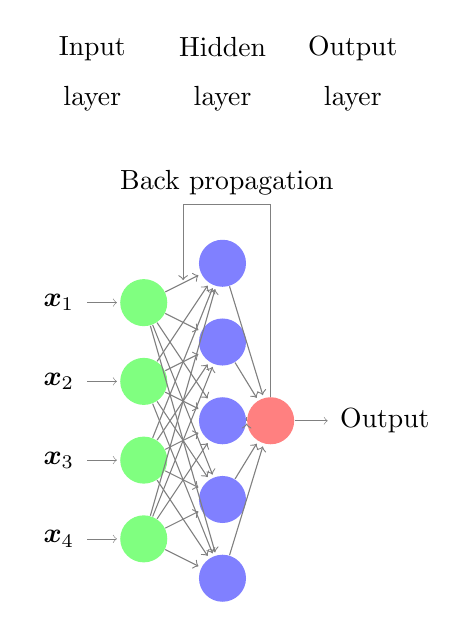
\begin{tikzpicture}[%
  shorten >=1pt,->,draw=black!50, node distance=\layersep,
  %every pin edge={<-,shorten <=1pt},
  neuron/.style={circle,fill=black!25,minimum size=17pt,inner sep=0pt},
  input neuron/.style={neuron, fill=green!50},
  output neuron/.style={neuron, fill=red!50},
  hidden neuron/.style={neuron, fill=blue!50},
  annot/.style = {text width=4em, text centered}
  ]
  % Draw the input layer nodes
  \foreach \name / \y in {1,...,4}
  % This is the same as writing \foreach \name / \y in {1/1,2/2,3/3,4/4}
  \node[input neuron, pin={[pin edge={<-,shorten <=1pt}]left: $\bm{x}_\y$}] (I-\name) at (0,-\y) {};

  % Draw the hidden layer nodes
  \foreach \name / \y in {1,...,5}
  \node[hidden neuron] (H-\name) at (\layersep,-\y cm+0.5cm) {};

  % Draw the output layer node
  \node[output neuron,pin={[pin edge={->}]right:Output}, right=of H-3] (O) {};

  % Connect every node in the input layer with every node in the
  % hidden layer.
  \foreach \source in {1,...,4}
  \foreach \dest in {1,...,5}
  \path (I-\source) edge (H-\dest);

  % Connect every node in the hidden layer with the output layer
  \foreach \source in {1,...,5}
  \path (H-\source) edge (O);

  % Annotate the layers
  \node[annot,above=15mm of H-1] (hl) {Hidden layer};
  \node[annot,left=of hl] {Input layer};
  \node[annot,right=of hl] {Output layer};
  %%% 
  \coordinate (H-I-1) at ($(H-1)!0.5!(I-1)$);
  \draw (O) |- ($(H-I-1) +(0,1)$) node[above,pos=0.75]{Back propagation} -- (H-I-1);
\end{tikzpicture}
\caption{Network diagram for one hidden layer neural network}
\label{fig:hidden}
\end{figure}
These values are again linearly combined to give {output unit activations}
\begin{equation}\label{z2}
\bm{z}^{[2]} = \bm{W}^{[2]}\bm{a}^{[1]} + \bm{b}^{[2]}
\end{equation}
This transformation corresponds to the second layer of the network. Finally, the output unit activations are transformed using an appropriate activation function to give a set of network output $\hat{y}$. The choice of activation function is determined by the nature of the data and the assumed distribution of target variables. 

Activations refers to the values that different layers of the neural network are passing to subsequent layers. So the input layer passes on the values $\bm{X}$ to the hidden layer with activation $\bm{a}^{[0]}$, hidden layer would in turn generate activation $\bm{a}^{[1]}$. First node generates $a^{[1]}_1$, second node generates $a^{[1]}_2$, and so on, i.e.,
\[
\bm{a}^{[1]} = \left[\begin{array}{c}
					a^{[1]}_1 \\
					a^{[1]}_2 \\
					a^{[1]}_3 \\
					a^{[1]}_4
				   \end{array}\right]
\]
with parameters $\bm{w}^{[1]}$ and $\bm{b}^{[1]}$. The output layer would generate $a^{[2]}\in\mathbb{R} = \hat{y}$ with parameters $\bm{w}^{[2]}$ and $b^{[2]}$.

Let $n^{[i]}$ be the number of nodes at layer $i$. The dimension of the parameters $\bm{W}^{[1]}$, $\bm{b}^{[1]}$, $\bm{W}^{[2]}$ and $\bm{b}^{[2]}$ depends on $n^{[i]}$ at different layers. The dimensions are 
\begin{multicols}{2}
\begin{itemize}[label=-]
\item $\bm{W}^{[1]}$ - $(n^{[1]},n^{[0]})$
\item $\bm{W}^{[2]}$ - $(n^{[2]},n^{[1]})$
\item $\bm{b}^{[1]}$ - $(n^{[1]},1)$
\item $\bm{b}^{[2]}$ - $(n^{[2]},1)$
\end{itemize}
\end{multicols}
\noindent For example, in Figure (\ref{fig:hidden}), the dimensions of the parameters would be
\begin{multicols}{2}
\begin{itemize}[label=-]
\item $\bm{W}^{[1]}$ - $(4,3)$
\item $\bm{W}^{[2]}$ - $(1,4)$
\item $\bm{b}^{[1]}$ - $(4,1)$
\item $\bm{b}^{[2]}$ - $(1,1)$
\end{itemize}
\end{multicols}
\begin{rem}
\normalfont 
\begin{enumerate}
\item This process of moving from the input to the output layer is known as {forward propagation}.
\item The number of nodes in the input layer equals to the number of input variables in the data being processed. The number of nodes in the output layer equals the number of outputs associated with each inputs. 
\item If linear activation function is used in the layers of a neural network, the neural network outputs would be a linear function of the input, no matter how many layers the neural network has, since the composition of linear functions is also a linear function, hence, there would be no hidden layer in the neural network.
\item If a linear function is used in the hidden layers, and logistic sigmoid function is used in outer layer, then the model would just be a standard logistic regression.
\item In practise, the optimal number of hidden layers and nodes depends on the nature of the problem. Some problem would require using trial and error method.
\item Although multiple hidden layers allows the network to build more and more abstract representation of the input variables, it comes at a price of needing more data, otherwise the network overfits, i.e., the network will `memorise' the data.
\item Some machine learning problem requires multiple nodes in the output layer, but our focus in this work would be problems that requires a single output in the output layer.
\end{enumerate}
\end{rem}

\section{Activation Functions}
When building a neural network, one of the choices to be made is what activation function to use in the hidden layer and output layer of the neural network. Different activation function can be used in different layer. In this section, we discuss some of the options for an activation function. 

\subsection{Logistic Sigmoid Function}
The logistic sigmoid function discussed in section \ref{sub:lsf} is one choice, the function is smooth and differentiable, this means that during back-propagation, the error can be back-propagated and the weights can be accordingly updated. The sigmoid is preferred in the outer layer for a binary classification, where $y\in\{0,1\}$, and we want $0\leq\hat{y}\leq 1$. The function is widely used but we still have some problems that needs to addressed. The gradient of the function is pretty flat beyond the $+3$ and $-3$ region (as seen in Figure (\ref{fig:sig_prime})), this means that once the function falls in that region the gradients become very small, which implies that network is not really learning in the region. Another problem that the sigmoid function suffers is that the values only range from $0$ to $1$. This means that the sigmoid function is not symmetric around the origin and the values received are all positive,and not all times would we desire the values going to the next node to be all of the same sign. This can be addressed by scaling the logistic sigmoid function to get the $\tanh$ function.
\newpage
\begin{figure}[htb!]
\centering 
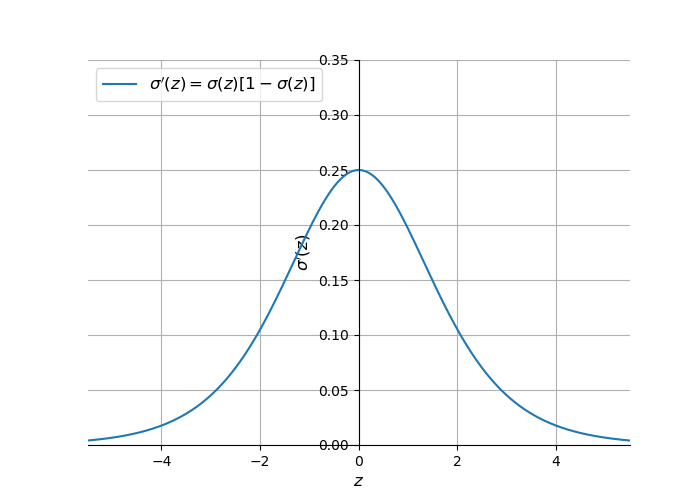
\includegraphics[scale=0.9]{png/sigmoid_prime.png} 
\caption{Gradient of logistic sigmoid function}
\label{fig:sig_prime}
\end{figure}


\subsection{Hyperpoblic Tangent Function}
The hyperbolic tangent ($\tanh$) function is also a sigmoid function similar to the logistic sigmoid function. It is actually just a scaled version of the logistic sigmoid function. It is given by 
\begin{equation}\label{eqn:tanh}
\tanh(z) = 2\sigma(2z) - 1 = \frac{e^z - e^{-z}}{e^z + e^{-z}}
\end{equation}
Its derivative is calculated thus;
\begin{equation}\label{eqn:tanh_prime}
\begin{split}
\frac{d}{dz}\tanh(z) &= \frac{(e^z + e^{-z})(e^z + e^{-z})-(e^z - e^{-z})(e^z - e^{-z})}{(e^z + e^{-z})^2} \\
	&= 1 - \frac{(e^z - e^{-z})^2}{(e^z + e^{-z})^2} \\
\tanh'(z)	&= 1 - \tanh^2(z)
\end{split}
\end{equation}
\begin{figure}[htb!]
\centering 
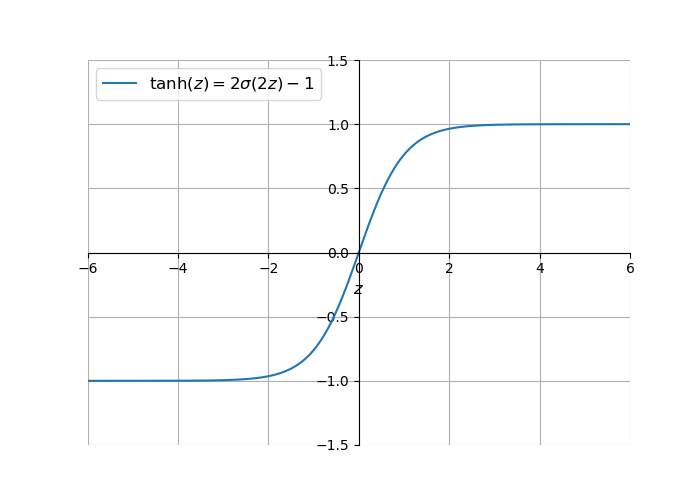
\includegraphics[scale=0.9]{png/tanh.png} 
\caption{$\tanh$ function}
\label{fig:tanh}
\end{figure}
For hidden units, $\tanh$ function almost always work better than the logistic sigmoid function because the values of the $\tanh$ function lies between $+1$ and $-1$ (as seen in Figure (\ref{fig:tanh})), hence the mean of the activations that come out from the hidden layer are closer to having mean $0$, rather than $0.5$ (for logistic sigmoid), which makes learning the outer layer a little bit easier. It is also continuous, differentiable and non linear, so errors can be easily backpropagated.
\begin{figure}[htb!]
\centering 
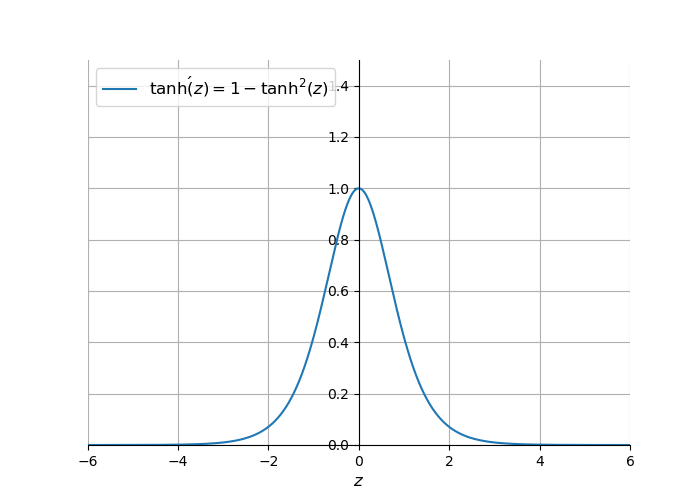
\includegraphics[scale=0.9]{png/tanh_prime.png} 
\caption{Gradient of $\tanh$ function}
\label{fig:tanh_prime}
\end{figure}

Sigmoidal units saturate across most of their domain; they saturate to a high value when $z$ is very positive, saturate to a low value when $z$ is very negative, and are only strongly sensitive to their input when $z$ is near $0$ {\cite{10.5555/3086952}}. This feature is a general problem for the sigmoidal functions, since large values snap to $1.0$ and small values snap to $-1$ or $0$ for $\tanh$ and logistic sigmoid respectively. Further, the functions are only really sensitive to changes around their mid-point of their input, such as $0.5$ for sigmoid and $0.0$ for $\tanh$. The limited sensitivity and saturation of the function happen regardless of whether the summed activation from the node provided as input contains useful information or not. Once saturated, it becomes challenging for the learning algorithm to continue to adapt the weights to improve the performance of the model. 

Finally, as the capability of hardware increased through GPUs very deep neural networks using logistic sigmoid and $\tanh$ activation functions could not easily be trained. Layers deep in large networks using these non-linear activation functions fail to receive useful gradient information. Error is back propagated through the network and used to update the weights. The amount of error decreases dramatically with each additional layer through which it is propagated, given the derivative of the chosen activation function. This is called the {vanishing gradient problem} and prevents deep (multi-layered) neural networks from learning effectively. Vanishing gradients make it difficult to know which direction the parameters should move to improve the cost function {\cite{10.5555/3086952}}.

\subsection{Rectified Linear Activation Function}
Although the use of non-linear activation functions allows neural networks to learn complex mapping functions, they effectively prevent the learning algorithm from working with deep networks. In order to use stochastic gradient descent with backpropagation of errors to train deep neural networks, an activation function is needed that looks and acts like a linear function, but is, in fact, a non-linear function allowing complex relationships in the data to be learned. The function must also provide more sensitivity to the activation sum input and avoid easy saturation. The solution is to use the rectified linear activation function. A node or neuron that implements this activation function is referred to as a {rectified linear activation unit} (ReLU) {\cite{Hahnloser}}; {\cite{Jarrett}}; {\cite{10.5555/3104322.3104425}}. Adoption of ReLU may easily be considered one of the few milestones in the deep learning revolution, e.g. the techniques that now permit the routine development of state-of-the-art deep neural networks {\cite{Krizhevsky}}. Currently, ReLU is the most successful and widely-used activation function.
\begin{figure}[htb!]
\centering 
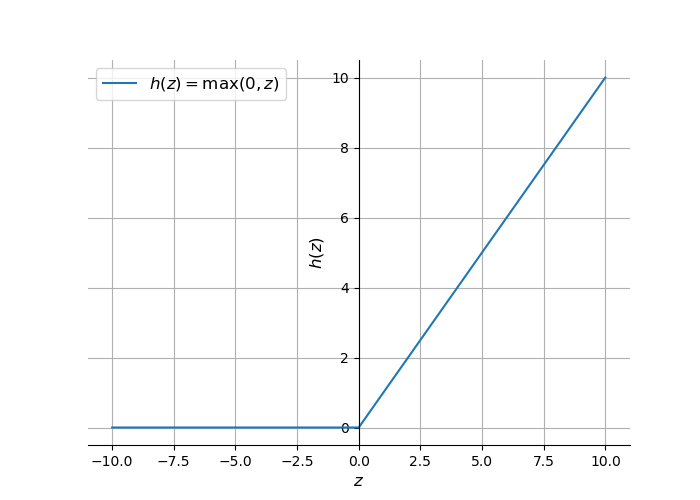
\includegraphics[scale=0.9]{png/relu.png} 
\caption{ReLU function}
\label{fig:relu}
\end{figure}
The rectified linear activation function is a simple calculation that returns the value provided as input directly, or the value $0$ if the input is $0$ or negative. The function is given by 
\begin{equation}\label{eqn:relu}
h(z) = \max(0,z)
\end{equation}
The function is linear for values greater than zero, meaning it has a lot of the desirable properties of a linear activation function when training a neural network using backpropagation. Yet, it is a non-linear function as negative values are always output as zero. Some advantages of using the rectified linear activation function are:
\begin{enumerate}[label=(\alph*)]
\item The rectifier function is trivial to implement, requiring a $\max()$ function. This is unlike the sigmoidal activation functions that require the use of an exponential calculation.
\item It does not activate all the nodes at the same time. Looking at the ReLU function (Figure (\ref{fig:relu})) if the input is negative it will convert it to zero and the node does not get activated. This means that at a time only a few nodes are activated making the network sparse which makes it efficient and easy for computation.
\item An important benefit of the rectifier function is that it is capable of outputting a true zero value. This is unlike the sigmoidal activation functions that learn to approximate a zero output, i.e., a value very close to zero, but not a true zero value. This means that negative inputs can output true zero values allowing the activation of hidden layers in neural networks to contain one or more true zero values. This is called a {sparse representation} and is a desirable property in representational learning as it can accelerate learning and simplify the model.
\item The rectified linear activation function mostly looks and acts like a linear activation function. Because rectified linear units are nearly linear, they preserve many of the properties that make linear models easy to optimise with gradient-based method, they also preserve many of the properties that make linear models generalise well {\cite{10.5555/3086952}}. 
\item The discovery and adoption of the rectified linear activation function meant that it became possible to exploit improvements in hardware and successfully train deep multi-layered networks with a non-linear activation function using backpropagation.
\end{enumerate}
Its derivative is given by:
\begin{equation}\label{eqn:relu_prime}
h'(z) = \left\{\begin{array}{lcr}
		1 & \text{if} & z \geq 0 \\
		0 & \text{if} & z < 0
		\end{array}\right.
\end{equation}
\begin{figure}[htb!]
\centering 
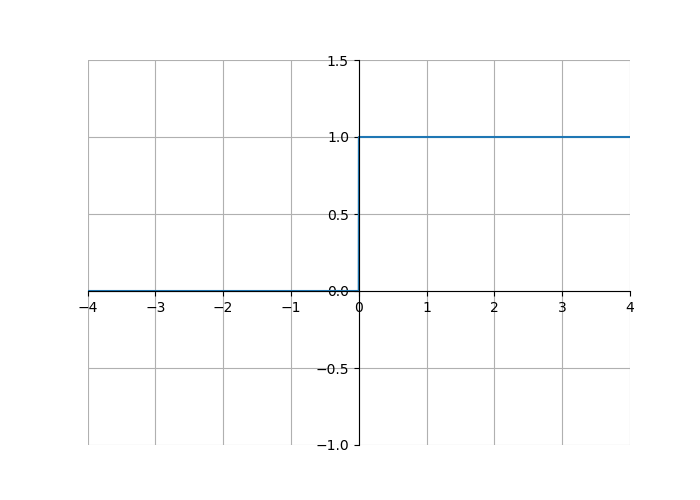
\includegraphics[scale=0.9]{png/relu_prime.png} 
\caption{Gradient of ReLU}
\label{fig:relu_prime}
\end{figure}
Because of the horizontal line in ReLU, for negative values (Figure (\ref{fig:relu})), the gradient can go towards $0$. For activations in that region of ReLU, gradient will be $0$ because of which the weights will not get adjusted during descent. That means, those nodes which go into that state will stop responding to variations in error or input (simply because gradient is $0$, nothing changes). This is called  {dying ReLU problem}. This problem can cause several nodes to just die and not respond making a substantial part of the network passive. There are variations in ReLU to mitigate this issue by simply making the horizontal line into non-horizontal component. We investigate some of these variations;
\begin{figure}[htb!]
\centering 
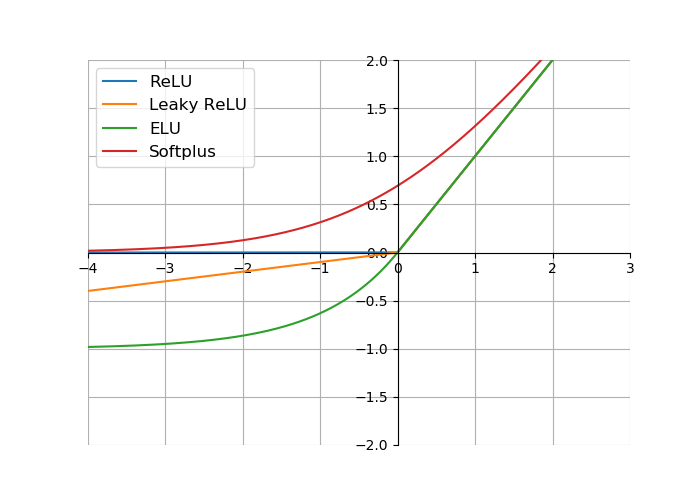
\includegraphics[scale=0.9]{png/compare.png} 
\caption{ReLU and some of its common variations}
\label{fig:compare}
\end{figure}
\begin{itemize}
\item Leaky ReLU (LReLU) {\cite{Maas2013}}:
\begin{equation}\label{eqn:lrelu}
f(z) = \left\{\begin{array}{lcr}
		z & \text{if} & z \geq 0 \\
		\alpha z & \text{if} & z < 0
		\end{array}\right.
\end{equation}
where $\alpha=0.01$. LReLU enables a small amount of information to flow to the next layer when $x < 0$.
\item Parametric ReLU (PReLU) {\cite{10.1109/ICCV.2015.123}}: The same form as LReLU but $\alpha$ is a learnable parameter. The network also learns the value of $\alpha$ for faster and more optimum convergence. Each channel has a shared $\alpha$ which is initialized to $0.25$.  PReLU function is used when the LReLU function still fails to solve the problem of dead nodes and the relevant information is not successfully passed to the next layer.
\item Softplus {\cite{10.5555/3104322.3104425}}: 
\begin{equation}
f(z) = \log(1 + \exp(z))
\end{equation}
Softplus can be viewed as a smooth version of ReLU.
\item Exponential Linear Unit (ELU) {\cite{Clevert2015FastAA}}:
\begin{equation}\label{eqn:elu}
f(z) = \left\{\begin{array}{lcr}
		z & \text{if} & z \geq 0 \\
		\alpha(\exp(z)-1) & \text{if} & z < 0
		\end{array}\right.
\end{equation}
where $\alpha=0.1$.
\item Scaled Exponential Linear Unit (SELU) {\cite{DBLP:journals/corr/KlambauerUMH17}}:
\begin{equation}\label{eqn:selu}
f(z) = \lambda\left\{\begin{array}{lcr}
		z & \text{if} & z \geq 0 \\
		\alpha(\exp(z)-1) & \text{if} & z < 0
		\end{array}\right.
\end{equation}
where $\alpha \approx 1.6733$ and $\lambda \approx 1.0507$.
\end{itemize}



\subsection{Swish Activation Function}
Swish is a new, self-gated activation function discovered by researchers at Google {\cite{DBLP:journals/corr/abs-1710-05941}}. It was shown that Swish consistently matches or outperforms ReLU on deep networks applied to a variety of challenging domains such as image classification and machine translation. On ImageNet, replacing ReLUs with Swish units improves top-1 classification accuracy by $0.9\%$. The Swish function is given by:
\begin{equation}\label{eqn:swish}
\varphi(z) = z\cdot\sigma(z)
\end{equation}
where $\sigma(z)$ is the sigmoid function as defined in \eqref{eqn:sigma}.

Like ReLU, Swish is unbounded above and bounded below. Unlike ReLU, Swish is smooth and non-monotonic. The non-monotonicity property of Swish distinguishes itself from most common activation functions. The derivative of Swish is
\begin{equation}\label{eqn:swish_prime}
\begin{split}
\varphi^{\prime}(z) &=\sigma(z)+ z \cdot \sigma(z)(1-\sigma(z)) \\
	&=\sigma(z)+z \cdot \sigma(z)-z \cdot \sigma(z)^{2} \\
	&=z \cdot \sigma(z)+\sigma(z)(1-z \cdot \sigma(z)) \\
\varphi^{\prime}(z)	&=\varphi(z)+\sigma(z)(1-\varphi(z))
\end{split}
\end{equation}
\begin{figure}[htb!]
\centering 
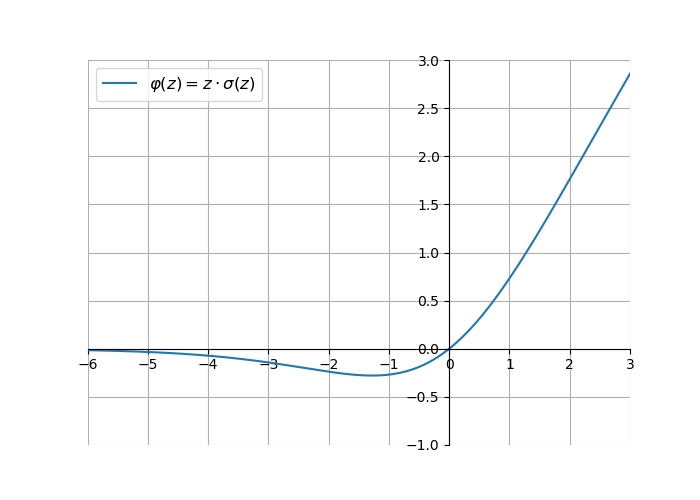
\includegraphics[scale=0.9]{png/swish.png} 
\caption{Swish function}
\label{fig:swish}
\end{figure}

An additional connection with ReLU can be seen if Swish is slightly reparameterized as follows:
\[
\varphi(z;\beta) = 2z\cdot \sigma(\beta z)
\]
If $\beta= 0$, Swish becomes the linear function $f(z) = z$. As $\beta \rightarrow \infty$, the sigmoid approaches a $0-1$ function, so Swish becomes like the ReLU function. This suggests that Swish can be loosely viewed as a smooth function, which non-linearly interpolates between the linear function and the ReLU function. The degree of interpolation can be controlled by the model if $\beta$ is set as a trainable parameter. This variant, without the factor of 2, is called {Swish-$\beta$}.

The paper by {\cite{DBLP:journals/corr/abs-1710-05941}} outlines the benefits of Swish;
\begin{itemize}[label=-]
\item It is bounded below. Swish therefore benefits from sparsity similar to ReLU. Very negative weights are simply zeroed out.
\item It is unbounded above. This means that for very large values, the outputs do not saturate to the maximum value (i.e., to $1$ for all the nodes). The ReLU function was such a large improvement over $\tanh$ because it is unbounded above, which avoids saturation whenever $z > 0$. This property is so important that almost every recently-proposed successful activation function is unbounded above. Swish shares this property, with its positive side approaching the linear function as the input becomes more positive.
\item The fact that Swish is a smooth curve means that its output landscape will be smooth. This provides benefits when optimizing the model in terms of convergence towards the minimum loss.
\begin{figure}[htb!]
\centering 
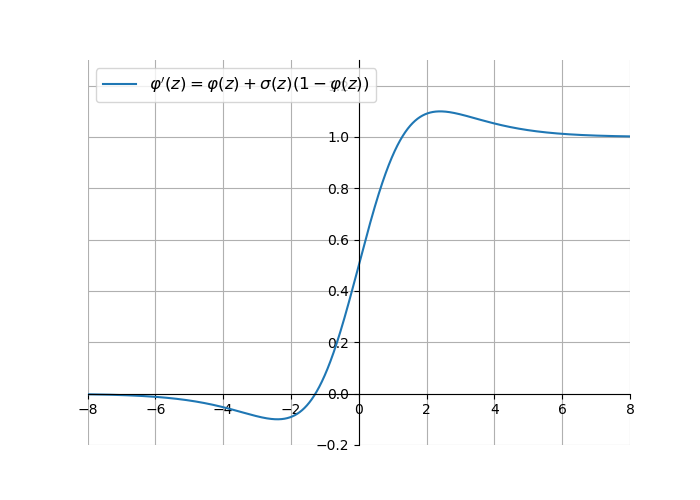
\includegraphics[scale=0.9]{png/swish_prime.png} 
\caption{Gradient of swish function}
\label{fig:swish_prime}
\end{figure}
\item Small negative values are zeroed out in ReLU (since $h(z) = 0$ for $z < 0$). However, those negative values may still be relevant for capturing patterns underlying the data. Swish nonetheless differs from ReLU  because it produces negative outputs for small negative inputs due to its non-monotonicity. The non-monotonicity of Swish improves gradient flow, which is important since it avoids dead nodes.
\end{itemize}

\subsection{Softmax Function}
The softmax function is also a type of sigmoid function but is handy when we are trying to handle classification problems. The sigmoid function as we saw earlier was able to handle just two classes. The softmax function can handle multiple classes, it would squeeze the outputs for each class between $0$ and $1$ and would also divide by the sum of the outputs. This essentially gives the probability of the input being in a particular class. The standard (unit) softmax function $\sigma :\mathbb{R}^{K}\to \mathbb{R}^{K}$ is defined by the formula:
\begin{equation}\label{eqn:softmax}
\sigma (\bm{z} )_{i}={\frac {e^{z_{i}}}{\sum _{j=1}^{K}e^{z_{j}}}}{\text{ for }}i=1,\dotsc ,K{\text{ and }}\bm{z} =(z_{1},\dotsc ,z_{K})\in \mathbb {R} ^{K}
\end{equation}
Prior to applying softmax, some vector components could be negative, or greater than one; and might not sum to 1; but after applying softmax, each component will be in the interval $(0,1)$, and the components will add up to $1$, so that they can be interpreted as probabilities. Furthermore, the larger input components will correspond to larger probabilities. Typically, Softmax is used only for the output layer, for neural networks that need to classify inputs into multiple categories. It is frequently appended to the last layer of an image classification network such as  VGG16 used in ImageNet competitions.

\section{Backpropagation}
In order to apply the stochastic gradient descent algorithm to optimise the parameters of a neural network, we need to calculate the gradient of an objective function with respect to the parameters of the network. Backpropagation refers to the method of calculating the gradient of neural network parameters using the calculus chain rule. The core insight is that the objective function derivative with respect to a module's input can be computed by working backwards from the gradient with respect to that module's output (or the corresponding module's input) (Figure \ref{fig:wahala}). The backpropagation equation can be repeatedly applied to propagate gradients through all modules, starting from the output at the top (where the network produces its 

\def\layersep{2.5cm}
\begin{landscape}
\begin{figure}[t]
\begin{tikzpicture}[node distance=\layersep, auto, >=latex']
    \tikzstyle{process} = [rectangle, minimum width=3cm, minimum height=1cm, text centered, draw=black]
    \tikzstyle{arrow} = [thick,->,>=stealth]
    \node (1) [process] {$\mathbf{z}^{[1]} = \mathbf{W}^{[1]}\mathbf{x} + \mathbf{b}^{[1]}$};
    \node (2) [process, right of=1, xshift=2cm] {$\mathbf{a}^{[1]} = g^{[1]}(\mathbf{z}^{[1]})$};
    \node (3) [process, right of=2, xshift=2cm] {$\mathbf{z}^{[2]} = \mathbf{W}^{[2]}\mathbf{a}^{[1]} + \mathbf{b}^{[2]}$};
    \node (4) [process, right of=3, xshift=2cm] {$a^{[2]} = \sigma(\mathbf{z}^{[2]})$};
    \node (5) [process, right of=4, xshift=2cm] {$\mathcal{L}(a^{[2]},y)$};
    \draw[<-] ([yshift=0pt]1.west)  -- node[above]{$\mathbf{W}^{[1]} \qquad\qquad$} ++(-4em,0em);
    \draw[<-] ([yshift=2pt]1.west)  -- node[right]{$\mathbf{x}$} ++(-3em,3em);
    \draw[<-] ([yshift=-2pt]1.west)  -- node[below]{$\mathbf{b}^{[1]} \qquad\qquad$} ++(-4em,-4em);
    \draw[<-] ([yshift=2pt]3.west)  -- node[above]{$\mathbf{W}^{[2]} \qquad\qquad\quad$} ++(-4em,4em) ;
    \draw[<-] ([yshift=-2pt]3.west)  -- node[below]{$\mathbf{b}^{[2]} \qquad\qquad$} ++(-4em,-4em);
    \draw [arrow] (1) -- (2);
    \draw [arrow] (2) -- (3);
    \draw [arrow] (3) -- (4);
    \draw [arrow] (4) -- (5);
    \draw[->] ([yshift=-4pt]5.west)  -- node[below]{} ++(-3.5em,0em);
    \draw[->] ([yshift=-4pt]4.west)  -- node[below]{} ++(-2.6em,0em);
    %\draw[->] ([yshift=-4pt]3.west)  -- node[below]{} ++(-4em,0em);
    \draw[->] ([yshift=-4pt]2.west)  -- node[below]{} ++(-3em,0em);
\end{tikzpicture}

\begin{minipage}[b]{.2\linewidth}
\[\begin{split}
\frac{\partial \mathcal{L}}{\partial \mathbf{z}^{[1]}} &= \frac{\partial \mathbf{z}^{[2]}}{\partial \mathbf{a}^{[1]}} \cdot \frac{\partial \mathcal{L}}{\partial \mathbf{z}^{[2]}} \cdot \frac{\partial \mathbf{a}^{[1]}}{\partial \mathbf{z}^{[1]}} \\
	&= \mathbf{W}^{{[2]}^T} \frac{\partial \mathcal{L}}{\partial \mathbf{z}^{[2]}} * g^{[1]'}(\mathbf{z}^{[1]})
\end{split}\]
\[\begin{split}
\frac{\partial \mathcal{L}}{\partial \mathbf{W}^{[1]}} &= \frac{\partial \mathcal{L}}{\partial \mathbf{z}^{[1]}} \cdot \frac{\partial \mathbf{z}^{[1]}}{\partial \mathbf{W}^{[1]}} \\
	&=  \frac{\partial \mathcal{L}}{\partial \mathbf{z}^{[1]}} \cdot \mathbf{x}^T
\end{split}\]
\[\begin{split}
\frac{\partial \mathcal{L}}{\partial \mathbf{b}^{[1]}} &= \frac{\partial \mathcal{L}}{\partial \mathbf{z}^{[1]}} \cdot \frac{\partial \mathbf{z}^{[1]}}{\partial \mathbf{b}^{[1]}} \\
	&=  \frac{\partial \mathcal{L}}{\partial \mathbf{z}^{[1]}} 
\end{split}\]
\end{minipage}
\hfill
\begin{minipage}[b]{.2\linewidth}
\[ 
\frac{d \mathbf{a}^{[1]}}{d \mathbf{z}^{[1]}} = g^{[1]'}(\mathbf{z}^{[1]})
\]
\vskip 4.5cm
{.}
\end{minipage}
\hfill
\begin{minipage}[b]{.2\linewidth}
\[\begin{split}
\frac{\partial \mathcal{L}}{\partial \mathbf{z}^{[2]}} &= \frac{\partial \mathcal{L}}{\partial a^{[2]}} \cdot \frac{d a^{[2]}}{d \mathbf{z}^{[2]}}  \\
	&= a^{[2]} - y
\end{split}\]

\[\begin{split}
\frac{\partial \mathcal{L}}{\partial \mathbf{W}^{[2]}} &= \frac{\partial \mathcal{L}}{\partial \mathbf{z}^{[2]}} \cdot \frac{\partial \mathbf{z}^{[2]}}{\partial \mathbf{W}^{[2]}} \\
	&=  \frac{\partial \mathcal{L}}{\partial \mathbf{z}^{[2]}} \cdot \mathbf{a}^{[1]}
\end{split}\]

\[\begin{split}
\frac{\partial \mathcal{L}}{\partial \mathbf{b}^{[2]}} &= \frac{\partial \mathcal{L}}{\partial \mathbf{z}^{[2]}} \cdot \frac{\partial \mathbf{z}^{[2]}}{\partial \mathbf{b}^{[2]}} \\
	&=  \frac{\partial \mathcal{L}}{\partial \mathbf{z}^{[2]}} 
\end{split}\]
\end{minipage}
\hfill
\begin{minipage}[b]{.2\linewidth}
{ }
\end{minipage}
\vskip 3cm 
.
\caption{Forward and backward propagation in a neural network layer}
\label{fig:wahala}
\end{figure}
\end{landscape}
\noindent 
prediction) all the way down (where the external input is fed). Once these gradients are determined, the computation of the gradients with respect to the weights of each element is straightforward. For a one hidden layer neural network to solve a binary classification problem, with parameters
\begin{multicols}{2}
\begin{itemize}[label=-]
\item $\bm{W}^{[1]}$ with shape $(n^{[1]},n^{[0]})$ 
\item $\bm{W}^{[2]}$ with shape $(n^{[2]},n^{[1]})$
\item $\bm{b}^{[1]}$ with shape $(n^{[1]},1)$
\item $\bm{b}^{[2]}$ with shape $(n^{[2]},1)$
\end{itemize}
\end{multicols}
\noindent
with cost function 
\[
J(\bm{W}^{[1]},\bm{b}^{[1]},\bm{W}^{[2]},\bm{b}^{[2]}) = \frac{1}{m}\sum_{i=1}^m \mathcal{L}(\hat{y},y)
\]
where $\mathcal{L}(\hat{y},y)$ is the loss function defined in equation \eqref{eqn:loss}.

Figure (\ref{fig:wahala}) shows the network gradients for a single training example. To train multiple training examples, we vectorise across different training examples;
\begin{equation}\label{eqn:train3}
\bm{Z}^{[1]} = \left[\begin{array}{cccc}
		 | & | &  & | \\
		 \bm{z}^{[1](1)} & \bm{z}^{[1](2)} & \hdots & \bm{z}^{[1](m)} \\
		 | & | &  & |
		 \end{array}\right]
\end{equation}
Similarly,
\begin{equation}\label{eqn:train4}
\bm{Z}^{[2]} = \left[\begin{array}{cccc}
		 | & | &  & | \\
		 \bm{z}^{[2](1)} & \bm{z}^{[2](2)} & \hdots & \bm{z}^{[2](m)} \\
		 | & | &  & |
		 \end{array}\right]
\end{equation}
Hence,
\[
\bm{Z}^{[1]}  = \bm{W}^{[1]} \bm{X} + \bm{b}^{[1]}; \qquad \bm{A}^{[1]} = g^{[1]}(\bm{Z}^{[1]}); \qquad \bm{Z}^{[2]}  = \bm{W}^{[2]} \bm{A}^{[1]} + \bm{b}^{[2]}; \qquad \bm{A}^{[2]} = g^{[2]}(\bm{Z}^{[2]})
\]
The gradients would be;
\begin{tasks}[label = {}](2)
\task $\dfrac{\partial J}{\partial \bm{Z}^{[2]}} = \bm{A}^{[2]} - \bm{y} $
\task $ \dfrac{\partial J}{\partial \bm{W}^{[2]}} = \dfrac{1}{m}  \dfrac{\partial J}{\partial \bm{Z}^{[2]}} \bm{A}^{[1]^T} $
\task $ \dfrac{\partial J}{\partial \bm{b}^{[2]}} = \dfrac{1}{m}\sum\limits_{i=1}^m \bm{A}^{[2]{(i)}} - \bm{y}^{[i]} \dfrac{\partial J}{\partial \bm{Z}^{[2](i)}} $
\task $ \dfrac{\partial J}{\partial \bm{Z}^{[1]}} = \bm{W}^{[2]^T} * g^{[1]^{\prime}}( \bm{Z}^{[1]}) $
\task $ \dfrac{\partial J}{\partial \bm{W}^{[1]}} = \dfrac{1}{m} \dfrac{\partial J}{\partial \bm{Z}^{[1]}} \bm{X}^T $
\task $ \dfrac{\partial J}{\partial \bm{b}^{[1]}} = \dfrac{1}{m} \sum\limits_{i=1}^m \dfrac{\partial J}{\partial \bm{Z}^{[1](i)}} $
\end{tasks}
where $*$ is the element-wise product of two matrices. The above operations matches the dimensions of the matrices.

In general, for an $L$ layer neural network, $L > 0$, which has $L-1$ hidden layers and $1$ input and output layer each. The parameters (weights and biases) for layer $l = 1,2,\hdots,L$ are represented as
\begin{multicols}{2}
\begin{itemize}[label=-]
\item $\bm{W}^{[l]}$ with shape $(n^{[l]},n^{[l-1]})$ 
\item $\bm{b}^{[l]}$ with shape $(n^{[l]},1)$
\end{itemize}
\end{multicols}
\noindent
where $n^{[l]}$ is the number of nodes in layer $l$, and $n^{[0]}$ is the number of nodes in the input layer. Hence, forward propagation would be;
\[
\begin{split}
\bm{Z}^{[l]}  &= \bm{W}^{[1]} \bm{A}^{[l-1]} + \bm{b}^{[l]} \\
 \bm{A}^{[l]} &= g^{[l]}(\bm{Z}^{[l]})
\end{split} 
\]
with $\bm{A}^{[0]}=\bm{X}$, and the backpropagation gradients are calculated thus;
\[
\begin{split}
\frac{\partial J}{\partial \bm{Z}^{[l]}} &= \dfrac{\partial J}{\partial \bm{A}^{[l]}} * g^{[l]^{\prime}}(\bm{Z}^{[l]}) \\
\dfrac{\partial J}{\partial \bm{W}^{[l]}} &= \dfrac{1}{m} \dfrac{\partial J}{\partial \bm{Z}^{[l]}} {\bm{A}^{[l-1]}}^T \\
\dfrac{\partial J}{\partial \bm{b}^{[l]}} &= \dfrac{1}{m} \sum\limits_{i=1}^m \dfrac{\partial J}{\partial \bm{Z}^{[l](i)}} \\
\dfrac{\partial J}{\partial \bm{A}^{[l-1]}} &= {\bm{W}^{[l]}}^T \frac{\partial J}{\partial \bm{Z}^{[1]}} 
\end{split}
\]

\subsection{Random Initialisation}
In neural networks, the weights are initialised with random number and the biases with zeros. If all the weights are initialized with $0$, the derivative with respect to cost function is the same for every $\bm{W}$ in the first layer of the network, thus all weights have the same value in subsequent iterations. This makes hidden units symmetric and continues for all the $k$ iterations i.e. setting weights to $0$ makes the model linear. In Python 3.7, \texttt{numpy.random.randn(n,m)} generates a $n\times m$ array of samples from the standard normal distribution, while \texttt{numpy.zeros((n,m))} generates a $n\times m$ array of zeros. To prevent the vanishing gradient problem, which makes learning takes a lot time, the initialised weight are multiplied by a small number (say $0.01$), so as to make the values going to the activation activation not too highly positive or highly negative, i.e.,
\[
\bm{W}^{[l]} = \texttt{numpy.random.randn}(n^{[l]},n^{[l-1]}) * 0.01
\]

Sometimes there can be better constants depending on the activation function used. {\cite{10.1109/ICCV.2015.123}} proposed activation aware initialization of weights (called He initialisation) used for ReLU activation that improved accuracy results on ImageNet classification task, the weights are initialised thus;
\[
\bm{W}^{[l]} = \texttt{numpy.random.randn}(n^{[l]},n^{[l-1]}) * \sqrt{\frac{2}{n^{[l-1]}}}
\]
Xavier initialisation is similar to He initialisation, it is used for $\tanh$ activation, and the weights are initialised as;
\[
\bm{W}^{[l]} = \texttt{numpy.random.randn}(n^{[l]},n^{[l-1]}) * \sqrt{\frac{1}{n^{[l-1]}}}
\]

\section{Convolutional Neural Networks}
Convolutional neural networks (CNNs) are similar to neural networks in that they consist of neurons which optimize themselves through learning, each neuron will still receive an input and perform an operation such as a scalar product followed by a non-linear function. They are designed to process data that are in form of multiple arrays, such as a color image consisting of three 2D arrays containing pixel intensities in three color channels; red, green and blue (RGB). CNN-based network architectures now dominate the field of computer vision and are pivotal in the rapid advancement of computer vision applications.

One of the challenges of computer vision problems is that inputs can get really big. For example, an input image of $1,000\times 1,000$ pixels, the dimension of the input features would be $1,000\times 1,000\times 3$ for its RGB channels. Hence, for a fully connected neural network with $1,000$  hidden units in the first layer, dimension of $\bm{W}^{[1]}$ is $(1,000,3\;\text{million})$. Getting enough data to train $3$ billion parameters without overfitting the network would be difficult, and also the computation and memory requirements needed to train the network is infeasible. Also, images with large pixel density would generally give more accurate results in computer vision applications. Our focus in this project would be on the applicability of CNNs in image data.

\subsection{Convolution Layer} \label{subsec:conv_layer}
In a convolutional layer, an input array and a convolution kernel array are combined to produce an array through a cross-correlation operation, a scalar bias is added to the array to produce an output, followed by a non-linear activation function (mostly ReLU) being applied to the output array. 

The cross-correlation operation is similar to the convolution between two functions $f,g:\mathbb{R}^n \rightarrow \mathbb{R}$, which is given by:
\begin{equation}\label{eqn:conv}
[f \circledast g](x) = 
\left\{\begin{array}{cc}
\displaystyle\int_{\mathbb{R}^n} f(z)g(x - z)\;\mathrm{d}z & \text{for continous variables} \\
\\
\displaystyle\sum_{a} f(a)g(x - a) & \text{for discrete variables}
\end{array}\right.
\end{equation}
That is, convolution is the measure of the overlap between $f$ and $g$ when one of the functions is shifted by $x$ and flipped. For a two-dimensional input image $\bm{I}$ and a two-dimensional kernel $\bm{K}$, convolution of $\bm{K}$ over $\bm{I}$ is given by:
\begin{equation}\label{eqn:2d_conv}
(\bm{I} \circledast \bm{K}) (i,j) = \sum_m \sum_n \bm{I}(m,n) \bm{K}(i-m,j-n)
\end{equation}
Cross-correlation operation $\star$, is the same as convolution but without flipping the kernel:
\begin{equation}\label{eqn:2d_cross}
(\bm{I} \star \bm{K}) (i,j) = \sum_m \sum_n \bm{I}(i+m,j+n) \bm{K}(m,n)
\end{equation} \noindent
% measures the displacement of one of the functions relative to the other, i.e., cross-correlation :
In a two-dimensional cross-correlation operation, a convolutional kernel (or filter) is positioned at the at the top-left corner of the input array and we slide it across the input array, both from left to right and top to bottom. When the kernel slides to a certain position, the input subarray contained in that position and the kernel array are multiplied elementwise and the resulting array is summed up yielding a single scalar value. This result if precisely the value of the output array at the corresponding location. Since the kernel has a width greater than one, and we can only compute the cross-correlation for locations where the kernel fits wholly within the image, the output size is given by the input size $H \times W$ minus the size of the convolutional kernel $h \times w$ via $(H - h + 1) \times (W - w + 1)$, since we need enough space to shift the convolutional kernel across the image. In practice, the height and width of the input image and convolution kernel are usually the same, hence, the height and width of the output would be of the same size $(H - h + 1)$.
\begin{figure}[H]
\centering
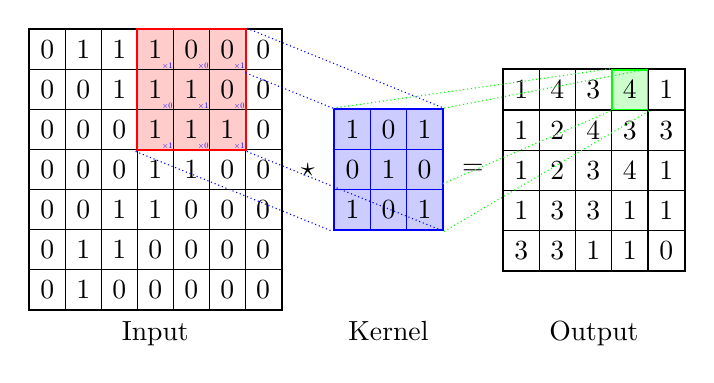
\begin{tikzpicture}[mmat/.style={matrix of math nodes,column sep=-\pgflinewidth/2,row sep=-\pgflinewidth/2,cells={nodes={draw,inner sep=4pt,thin}},draw=#1,thick,inner sep=0pt},
   mmat/.default=black,
   node distance=0.3em]
 \matrix[mmat](mat1){
         0 & 1 & 1 & 1 & 0 & 0 & 0 \\ 
         0 & 0 & 1 & 1 & 1 & 0 & 0 \\ 
         0 & 0 & 0 & 1 & 1 & 1 & 0 \\ 
         0 & 0 & 0 & 1 & 1 & 0 & 0 \\ 
         0 & 0 & 1 & 1 & 0 & 0 & 0 \\ 
         0 & 1 & 1 & 0 & 0 & 0 & 0 \\ 
         0 & 1 & 0 & 0 & 0 & 0 & 0 \\ 
         };
 \def\myarray{{1,0,1},{0,1,0},{1,0,1}}       
 \foreach \X in {0,1,2}
 {\foreach \Y in {0,1,2}
  {\pgfmathsetmacro{\myentry}{{\myarray}[\Y][\X]}
  \path (mat1-\the\numexpr\Y+1\relax-\the\numexpr\X+4\relax.south east)
  node[anchor=south east,blue,scale=0.3,inner sep=1.2pt]{$\times\myentry$};
  }}         
 \node[fit=(mat1-1-4)(mat1-3-6),inner sep=0pt,draw,red,thick,name path=fit](f1){};      
 \node[right=of mat1] (mul) {$\star$};      
 \matrix[mmat=blue,fill=blue!20,right=of mul,name path=mat2](mat2){    
     1 & 0 & 1 \\ 
     0 & 1 & 0 \\ 
     1 & 0 & 1 \\ };
 \node[right=of mat2] (eq) {$=$};       
 \matrix[mmat,right=of eq](mat3){    
     1 & 4 & 3 & |[draw=green,thick,fill=green!20,alias=4]|4 & 1 \\ 
     1 & 2 & 4 & 3 & 3 \\ 
     1 & 2 & 3 & 4 & 1 \\ 
     1 & 3 & 3 & 1 & 1 \\ 
     3 & 3 & 1 & 1 & 0 \\ 
 };
 \foreach \Anchor in {south west,north west,south east,north east}
 {\path[name path=test] (f1.\Anchor) -- (mat2.\Anchor);
 \draw[blue,densely dotted,name intersections={of=test and fit,total=\t}]
 \ifnum\t>0 (intersection-\t) -- (mat2.\Anchor) \else
  (f1.\Anchor) -- (mat2.\Anchor)\fi;
 \path[name path=test2]  (4.\Anchor) -- (mat2.\Anchor);  
 \draw[green,densely dotted,name intersections={of=test2 and mat2,total=\tt}] 
 \ifnum\tt>0 (intersection-1) -- (4.\Anchor) \else
    (mat2.\Anchor) --  (4.\Anchor)\fi;
    }
 \path (mat1.south) node[below] {Input}
  (mat2|-mat1.south) node[below] {Kernel}
  (mat3|-mat1.south) node[below] {Output};
 \begin{scope}[on background layer]
  \fill[red!20] (f1.north west) rectangle (f1.south east);
 \end{scope}
\end{tikzpicture}
\caption[Two-dimensional cross-correlation operation]{Two-dimensional cross-correlation operation. The shaded portions are the input, kernel array and fourth output elements,  used in its computation: $1\times 0+0\times 0+0\times 1+1\times 0+1\times 1+0\times 0+1\times 1+1\times 0+1\times 1=4$.}
\label{fig:cross_cor}
\end{figure}
\noindent 
With matrix multiplications in traditional neural networks, every output unit depends on every input unit, convolutional networks, however, typically have sparse interactions which is 
\begin{figure}[H]
\centering
	\begin{subfigure}[t]{\textwidth}
	\centering
	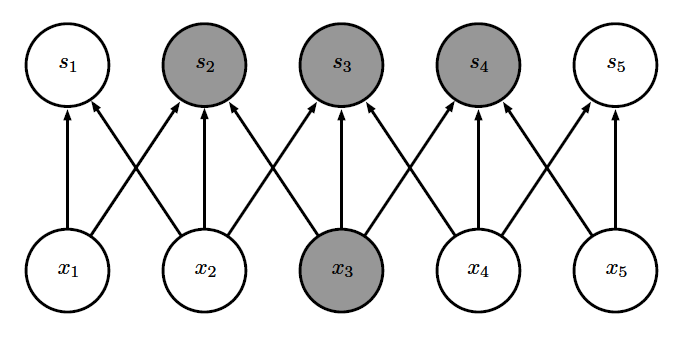
\includegraphics[scale=0.5]{png/sparse2.png}
 	\caption{When $\bm{s}$ is formed by convolution with a kernel of width $3$, only three outputs are affected by $\bm{x}$}	 
	\label{subfig:sparse1}
	\end{subfigure}
	
	\medskip
	
	\begin{subfigure}[t]{\textwidth}
	\centering
	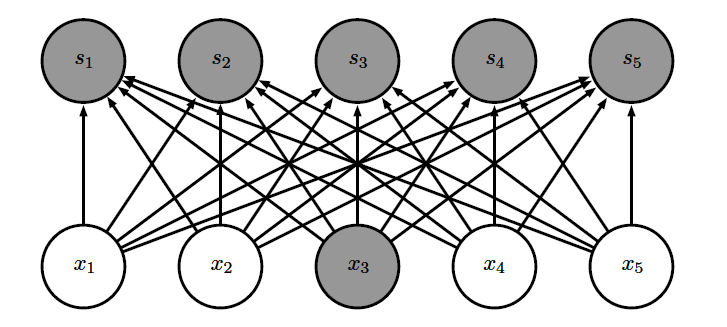
\includegraphics[scale=0.5]{png/sparse1.png}		
	\caption{When $\bm{s}$ is formed by matrix multiplication, connectivity is no longer sparse, so all the outputs are affected by $\bm{x}_3$}	 
	\label{subfig:sparse2}
	\end{subfigure}
\caption[Representation of sparse and full connectivity]{Representation of sparse and full connectivity, \protect{\cite{10.5555/3086952}}}	 
\label{fig:sparse}
\end{figure}
\noindent
accomplished by making the kernel smaller than the input. For example, when processing   an image, the input image might have thousands or millions of pixels, but small, meaningful features such as edges can be detected with kernels that occupy only tens or hundreds of pixels. This means that fewer parameters are stored, which both reduces the memory requirements of the model and improves its efficiency. These improvements in efficiency are usually quite large. Matrix multiplication used in traditional neural networks (Figure \ref{subfig:sparse2}) requires $m \times n$ parameters for $m$ inputs and $n$ outputs, which corresponds to $\mathcal{O}(m \times n)$ runtime (per example). Convolution networks limits the number of connections each output may have to $k$ (Figure \ref{subfig:sparse1}), then the sparsely connected approach requires only $k \times n$ parameters and $\mathcal{O}(k \times n)$ runtime, where $k $ is several orders of magnitude smaller than $m$. 

Convolution layers are also useful for local feature detection (such as edge detection by finding the locations of pixel change in the input), since a feature that is useful in one part of the image is probably useful in another part of the image. The lighter region in the middle of 
\begin{figure}[H]
\centering
	\begin{subfigure}[t]{\textwidth}
	\centering
	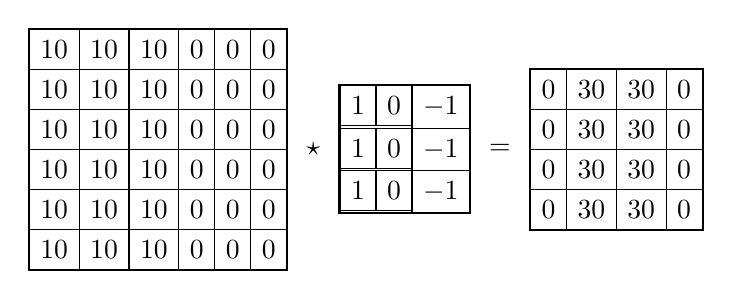
\begin{tikzpicture}[mmat/.style={matrix of math nodes,column sep=-		\pgflinewidth/2,row sep=-\pgflinewidth/2,cells={nodes={draw,inner sep=4pt,thin}},draw=#1,thick,inner sep=0pt},
   mmat/.default=black,
   node distance=0.3em]
	\matrix[mmat](mat1){
         10 & 10 & 10 & 0 & 0 & 0  \\ 
         10 & 10 & 10 & 0 & 0 & 0  \\ 
         10 & 10 & 10 & 0 & 0 & 0  \\ 
         10 & 10 & 10 & 0 & 0 & 0  \\ 
         10 & 10 & 10 & 0 & 0 & 0  \\ 
         10 & 10 & 10 & 0 & 0 & 0  \\ 
         };   
 	\node[right=of mat1] (mul) {$\star$};      
 	\matrix[mmat,right=of mul](mat2){    
     1 & 0 & -1 \\ 
     1 & 0 & -1 \\ 
     1 & 0 & -1 \\ };
 	\node[right=of mat2] (eq) {$=$};       
 	\matrix[mmat,right=of eq](mat3){    
     0 & 30 & 30 & 0  \\ 
     0 & 30 & 30 & 0  \\ 
     0 & 30 & 30 & 0  \\ 
     0 & 30 & 30 & 0  \\  
 	};
 	\end{tikzpicture}
 	\caption{Cross-correlating a vertical edge filter on an input image}	 
	\label{subfig:detection}
	\end{subfigure}
	
	\medskip
	
	\begin{subfigure}[t]{.7\linewidth}
	\centering
	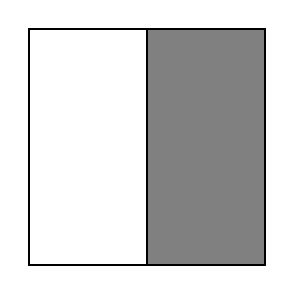
\begin{tikzpicture}[
    tlabel/.style={pos=0.4,right=-1pt},
    baseline=(current bounding box.center)
    ]	
	\draw[fill=white,thick](0,0) rectangle (3,3);
	\draw[fill=gray,thick] (1.5,0) rectangle (3,3);
	\end{tikzpicture}	
	\hspace{0.4mm}
	$\star$
	\hspace{0.4mm}
	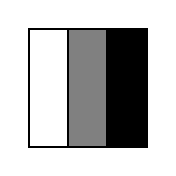
\begin{tikzpicture}[
    tlabel/.style={pos=0.4,right=-1pt},
    baseline=(current bounding box.center)
    ]
	\draw[fill=white,thick](0,0) rectangle (1.5,1.5);
	\draw[fill=gray,thick] (0.5,0) rectangle (1,1.5);
	\draw[fill=black,thick] (1,0) rectangle (1.5,1.5);
	\end{tikzpicture}
	\hspace{0.4mm}
	$=$
	\hspace{0.4mm}
	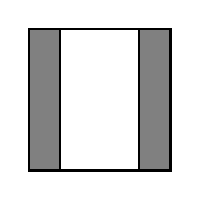
\begin{tikzpicture}[
    tlabel/.style={pos=0.4,right=-1pt},
    baseline=(current bounding box.center)
    ]
	\draw[fill=white,thick](0,0) rectangle (1.8,1.8);
	\draw[fill=gray,thick] (0,0) rectangle (0.4,1.8);
	\draw[fill=gray,thick] (1.4,0) rectangle (1.8,1.8);
	\end{tikzpicture}		
	\caption{Picture plots where bright halves gives brighter pixel intensity values, and darker halves gives darker pixel intensity values}	 
	\label{subfig:detection1}
	\end{subfigure}
\caption{Vertical edge detection}	 
\label{fig:detection}
\end{figure} 
\noindent
the output from Figure \ref{subfig:detection1} corresponds to the vertical edge filter (which consists of a $3 \times 3$ region where pixel intensity values are relatively bright on the left part and relatively dark on the right part) having detected a strong vertical edge down the middle of the input image, the light region shows a light to dark transition in the input image, a dark region would show a dark to light transition in the input image. Larger input images, such as $1,000 \times 1,000$ pixel image would give better edge detection results. Different filter values have been used for edge detection in computer vision literature, such as the Sobel filter {\cite{sobel19683x3}}, and the Scharr filter {\cite{jaehne1999k}}; with deep learning, the values of the edge filter $w_1,w_2,\hdots,w_9$ are treated as parameters which are learnt using back propagation, this enables the convolution layer to detect edges in different orientations. When training CNN models based on convolutional layers, the kernels are randomly initialized, just as we would with a fully-connected layer.  

\subsection{Padding and Stride}
In the previous example of Figure \ref{fig:cross_cor}, our input had both a height and width of $7$ and our convolution kernel had both a height and width of $3$, yielding an output representation with dimension $5 \times 5$, which follows the generalisation from Section \ref{subsec:conv_layer}.
% assuming that the input shape is $H \times W$ and the convolution kernel shape is $h \times w$, then the output shape will be $(H-h+1) \times (W-w+1)$. 
Hence, the output shape of the convolutional layer is determined by the shape of the input and the shape of the convolution kernel. 

Since kernels generally have width and height greater than $1$, after applying many successive convolutions, we tend to wind up with outputs that are considerably smaller than our input. If we start with a $240\times 240$ pixel image, $10$ layers of $5 \times 5$ convolutions reduce the image to $200 \times 200$ pixels, slicing $30\%$ off the image and with it obliterating all useful details about the borders of the original image. Padding is the most used tool for handling this issue. In other examples, if we find the original input resolution to be unhandy, we may want to significantly decrease the dimensionality, strided convolutions in these instances are a common technique that can aid.

One tricky issue when applying convolutional layers, as mentioned above, is that we tend to lose pixels on the boundary of our image. Since we usually use small kernels, we might only lose a few pixels for every given convolution, but this can add up as we apply several 
\begin{figure}[H]
\centering
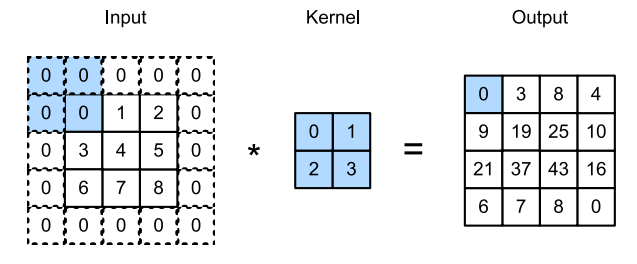
\includegraphics[scale=0.9]{png/padding.png}
\caption[Two-dimensional cross-correlation with padding]{Two-dimensional cross-correlation with padding, {\cite{zhang2020dive}}}
\label{fig:pad}
\end{figure} \noindent
successive convolutional layers. One easy solution to this problem is to add additional filler pixels around the boundary of our input image, thereby increasing the image's effective size. Typically, we set the values of the extra pixels to zero. In Figure \ref{fig:pad}, we pad a $3 \times 3$ input, increasing its size to $5 \times 5$. The corresponding output then increases to a $4 \times 4$ matrix. The shaded portions are the first output element as well as the input and kernel tensor elements used for the output computation: $0 \times 0 + 0 \times 1 + 0 \times 2 + 0 \times 3 = 0$. In general, if we add a total of $p$ number of padding around the input, the height and width of the output will be
\begin{equation} \label{eqn:pad}
\left(H - w + 2p + 1\right)
\end{equation} \noindent
In many cases, we will want to set $p = h - 1$ to give the input and output the same height and width. This will make it easier to predict each layer's output shape while building the network. 
%Assuming that $h$ is odd, we will pad $p_h/2$ rows on both sides of the height. If $h$ is even, we pad $\ceil*{p_h/2}$ rows on the top of the input and $\floor*{ph/2}$ rows on the bottom, and pad both sides of the width in the same way. 
CNNs commonly use convolution kernels with odd height and width values, choosing odd kernel sizes has the benefit that we can preserve the spatial dimensionality while padding with the same number of rows on top and bottom, and the same number of columns on left and right.

When computing the cross-correlation, we begin with the convolution window at the top-left corner of the input tensor, and then slide it both down and to the right over all locations, defaulting to sliding one element at a time in previous examples. However, often we shift our window more than one element at a time, skipping the intermediate positions, either for computational effectiveness or because we want to downsample. We refer to the number of rows and columns traversed per slide as the stride. So far, we have used strides of $1$, both 
\begin{figure}[H]
\centering
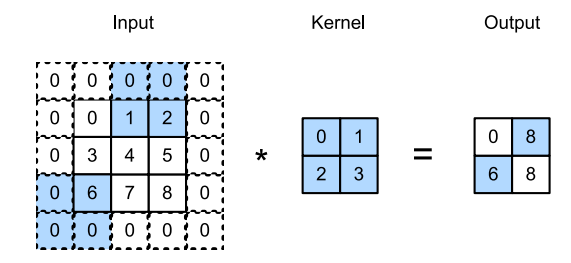
\includegraphics[scale=0.9]{png/stride.png}
\caption[Cross-correlation with strides of $3$ and $2$ for height and width respectively]{Cross-correlation with strides of $3$ and $2$ for height and width respectively, {\cite{zhang2020dive}}}
\label{fig:stride}
\end{figure} \noindent
for height and width. Sometimes, we may want to use a larger stride, Figure \ref{fig:stride} shows a two-dimensional cross-correlation operation with a stride of $3$ vertically and $2$ horizontally. The shaded portions are the output elements as well as the input and kernel tensor elements used for the output computation: $0 \times 0 + 0 \times 1 + 1 \times 2 + 2 \times 3 = 8, 0 \times 0 + 6 \times 1 + 0 \times 2 + 0 \times 3 = 6$. The convolution window slides two columns to the right when the second element of the first row is outputted. There is no output when the convolution window continues to slide two columns to the right on the input, since the input variable does not fill the window (unless we add another column of padding). In practice, we apply the same amount of stride vertically and horizontally. Hence, given an input image with size $H \times H$, a convolution kernel with size $h \times h$, applied at stride $s$ with pad $p$, the output would be of height and width
\begin{equation}\label{eqn:pad_stride}
\floor*{\dfrac{H + 2p - h}{s} + 1}
\end{equation}


\subsection{Multiple Input and Multiple Output Channels}
Before now, we have thought of the inputs, convolution kernels, and outputs each as two-dimensional tensors. But, color images have the standard RGB channels to indicate the amount of red, green and blue. Hence our our inputs and hidden representations both become three dimensional tensors when we consider the channels. For example, each RGB input image has shape $H \times H \times 3$, where the last axis with size $3$ is known as the channel dimension. In this section, we will take a deeper look at convolution kernels with multiple input and multiple output channels.

For input data containing multiple channels, we need to construct a convolution kernel with the same number of input channels as the input data, so that it can perform cross-correlation with the input data. Assuming that the number of channels for the input data is $c_i$, the number of input channels of the convolution kernel also needs to be $c_i$. When $c_i = 1$, the convolution kernel is just a two-dimensional tensor of shape $h \times h$. However, when $c_i > 1$, we need a kernel that contains a tensor of shape $h \times h$ for every input channel. Thus, we concatenate these $c_i$ tensors together to yields a convolution kernel of shape $h \times h \times c_i$. Since the input and convolution kernel each have $c_i$ channels, we can perform a cross-correlation operation on the two-dimensional tensor of the input and the two-dimensional tensor of the convolution kernel for each channel by summing over the channels to yield a two-dimensional tensor. 
\begin{figure}[H]
\centering
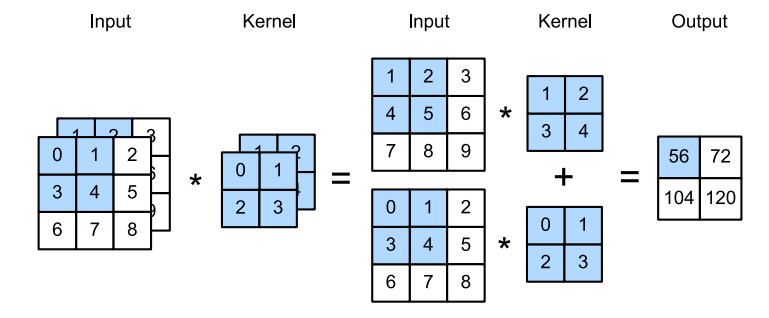
\includegraphics[scale=0.9]{png/cross_corr_2_dim.png}
\caption[Cross-correlation computation with $2$ input channels]{Cross-correlation computation with $2$ input channels, {\cite{zhang2020dive}}}
\label{fig:2-dim}
\end{figure} \noindent
Figure (\ref{fig:2-dim}) shows an example of a two-dimensional cross-correlation with two input channels. The shaded portions are the first output element as well as the input and kernel tensor elements used for the output computation: $(1\times 1+2\times 2+4\times 3+5\times 4)+(0\times 0+1\times 1+3\times 2+4\times 3) = 56 $.

We have always ended up with one output channel regardless of the number of input channels. However, it is essential to have multiple channels, so that each channel provides a set of learned features to the subsequent layer. Some channels could become skilled in identifying edges at lower layers that are closer to inputs, while others could identify textures. Also, in most popular neural network architectures, channel dimension is usually increased as the network gets deeper typically downsampling to trade off spatial resolution for greater channel depth. Let by $c_i$ and $c_0$ be the number of input and output channels, respectively, with kernel width of shape $h \times h$. To get an output with multiple channels, we can create a kernel tensor of shape $h \times h \times c_i$ for every output channel, we then concatenate them on the output channel dimension, so that the shape of the convolution kernel is $h \times h \times c_i \times c_0$. In cross-correlation operations, the result on each output channel is calculated from the convolution kernel corresponding to that output channel and takes input from all channels in the input tensor. The outcome on each output channel is determined from the convolution kernel corresponding to that output channel in cross-correlation operations and takes input from all channels in the input tensor.


\subsection{Pooling Layer}
Sometimes, as we process images, we want to progressively reduce the spatial resolution of our hidden representations, aggregating information so that the higher we go up in the network, the greater the input receptive field to which each hidden node is sensitive. By gradually aggregating information, creating larger and larger maps, we achieve the goal of eventually learning global representation, while at the same time retaining all the advantages of the convolutional layers in the intermediate layers of processing. In this section, pooling layers are studied, which serve the dual purpose of merging semantically similar features into one and of spatially downsampling representations.

Like convolutional layers, pooling operators consist of a fixed-shaped window that slides across all regions of the input according to its stride, computing a single output for each 
\begin{figure}[H]
\centering
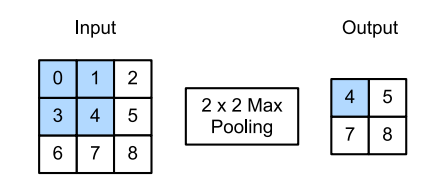
\includegraphics[scale=0.9]{png/pooling.png}
\caption[Maximum pooling with a pooling window shape of $2 \times 2$]{Maximum pooling with a pooling window shape of $2 \times 2$, {\cite{zhang2020dive}}}
\label{fig:pool}
\end{figure} \noindent
position crossed by the window. However, unlike the cross-correlation operation of inputs and kernels in the convolutional layer, the pooling layer does not include any parameters, i.e., there is no kernel. Instead, pooling operators are deterministic, usually measuring either the maximum (max pooling) or the average value (average pooling) of the elements in the pooling window. In both cases, as with the cross-correlation operator, the pooling window starts from the top left of the input tensor and slides through the input tensor from left to right and from top to bottom. The maximum or average value of the input sub-tensor in the window is determined at each position that the pooling window reaches, depending on whether the maximum or average pooling value is used. Figure \ref{fig:pool} shows a maximum pooling operation, the four elements are derived from the maximum value in each pooling window:
\begin{equation}
\begin{array}{ll}
\max (0,1,3,4)=4, & \max (1,2,4,5)=5, \\
\max (3,4,6,7)=7, & \max (4,5,7,8)=8. 
\end{array}
\end{equation} \noindent
As with convolutional layers, we can alter the polling operation to achieve a desired output shape by padding the input and adjusting the stride. When processing multi-channel input data, the pooling layer pools each input channel separately, rather than summing up inputs over channels as in a convolutional layer. This means that the number of input channels is the same as the number output channels of the pooling layer.


\section{Dropout}
Dropout {\cite{vsrivastava14a}} is a regularisation technique which involves injecting noise while computing each internal layer during forward propagation. In each forward pass, we randomly set some nodes to zero in each layer before calculating the subsequent layer., i.e., we dropout some neurons during training. The injected noise is added in an unbiased manner so that the expected value of each layer, while fixing the others, is equal to the value it would have taken absent noise. During dropout, each layer  normalised using the fraction of nodes that have been retained. In general, with dropout probability $p$, each intermediate activation $h$ is replaced by a random variable $h^{\prime}$ using the equation
\begin{equation}\label{eqn:dropout}
h^{\prime}=\left\{\begin{array}{ll}
0 & \text { with probability } p \\
\dfrac{h}{1-p} & \text { otherwise }
\end{array}\right.
\end{equation} \noindent 
with $\mathbb{E}[\;h^{\prime}\;] = h$, probability of dropping $p$ is a hyperparameter. Dropout helps reduce the number of learnable parameters in fully connected layers since some nodes are dropped, this helps speed up training of neural networks. Figure \ref{fig:dropout} shows a fully connected layer before and after dropout using $p=0.6$.
\begin{figure}[H]
\centering
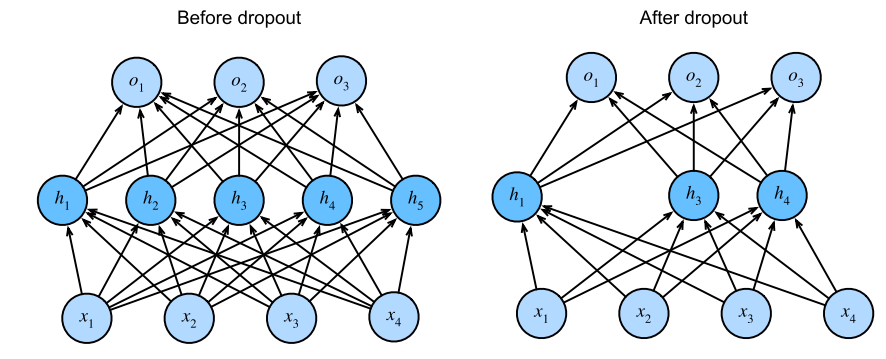
\includegraphics[scale=0.9]{png/dropout.png}
\caption[Fully connected layer before and after dropout]{Fully connected layer before and after dropout, {\cite{zhang2020dive}}}
\label{fig:dropout}
\end{figure}


\section{Batch Normalisation}
A number of practical challenges arises when training deep learning models. First, choices in pre-processing data often make a huge difference in the final results. Hence, we normalise the input layer, hidden layers should also be normalised. Second, if a model learns mapping $X \rightarrow Y$, if the distribution of $X$ changes, we might need to retrain the model by trying to align distribution of $X$ with distribution of $Y$. This drift in the distribution of the variables could hamper the convergence of the network, we might also need to make compensatory adjustments in the learning rates. Third, regularisation becomes more critical since deeper networks are complex and easily capable of overfitting.  

Batch Normalisation {\cite{ioffe15}}, tackles these challenges (and more) in two steps as follows: In each training iteration, normalise the inputs of preceding layers by subtracting the mean and dividing by their standard deviation, where both are estimated based on the statistics of the current minibatch. Next, we apply scale coefficient and shift offset, these operations maintains the expressive power of the network to learn whether to keep the original (or slightly different normalised) input or the normalised input when moving to the next layer. In general, if $\bm{x} \in \mathcal{B}$ is an input to batch normalisation (BN) that is from a minibatch $\mathcal{B}$, batch normalisation transforms $\bm{x}$ according to the equation:
\begin{equation} \label{eqn:batch_norm}
\mathrm{BN}(\bm{x})= \boldsymbol{\gamma} \odot \frac{\bm{x}-\hat{\boldsymbol{\mu}}_{\mathcal{B}}}{\hat{\boldsymbol{\sigma}}_{\mathcal{B}}}+\boldsymbol{\beta}
\end{equation} \noindent
where $\odot$ is the elementwise product operator, $\hat{\boldsymbol{\mu}}$ and $\hat{\boldsymbol{\sigma}}$ are the sample mean and sample standard deviation of minibatch $\mathcal{B}$ respectively, $\boldsymbol{\gamma}$ and $\boldsymbol{\beta}$ are the scale parameter and shift parameter respectively. These parameters are learnable parameters that have the same shape as $\bm{x}$. As a result, variable magnitudes for intermediate layers cannot diverge during training because the batch normalisation centers and rescales back to the specified mean and size. It also allows high learning rate since it makes sure there is no activation that gets really high or really low. $\hat{\boldsymbol{\mu}}$ and $\hat{\boldsymbol{\sigma}}$ are calculated using the equation
\begin{equation}\label{eqn:mean_variance}
\begin{array}{l}
\hat{\boldsymbol{\mu}}_{\mathcal{B}} = \displaystyle \frac{1}{|\mathcal{B}|} \sum_{\bm{x} \in \mathcal{B}} \bm{x} \\
\hskip 1pt
\hat{\boldsymbol{\sigma}}_{\mathcal{B}}^{2} = \displaystyle \frac{1}{|\mathcal{B}|} \sum_{\mathbf{x} \in \mathcal{B}}\left(\bm{x}-\hat{\boldsymbol{\mu}}_{\mathcal{B}}\right)^{2}+\epsilon
\end{array}
\end{equation} \noindent
A small $\epsilon > 0$ is added to the variance estimate to ensure that we never attempt to divide by zero, this extra constant adds noise estimates of the mean and variance to each hidden layer activations, similar to dropout which has helps in reducing overfitting. 

Batch normalisation layers are often used for convolutional layers, added after convolutional layers and before the non-linear activation functions. When the convolution has several output channels, we need to perform batch normalisation for each output of these channels, and each channel has its own scale and shift parameters, all of which are scalars. Assume that our minibatches contain $m$ examples and that for each channel, the output of the convolution is of size $q \times q$. For convolutional layers, each batch normalisation is carried out over the $m \times q \times q$ elements per output channel simultaneously. Thus, when calculating mean and variance, we collect values across all spatial locations and then apply the same mean and variance within the given channel to normalise the value at each spatial location.


\section{Gradient Descent Optimisation Algorithms}
We introduced minibatch stochastic gradient descent (SGD) in Section \ref{sec:sgd}, which improved on the convergence rate of gradient descent, where we made parameter updates using a minibatch with size $b$, instead of the whole dataset at each iteration. We showed that this optimiser has good convergence rate for smooth convex objective (loss) functions, using sufficiently small minibatch size $b$. In practice, common loss functions for neural networks are highly non-convex, minimising the loss becomes a challenge using SGD algorithms due to saddle points in the function {\cite{dauphin17e}}, saddle points are usually surrounded by a plateau of the same error, which makes it notoriously difficult for SGD to escape, as the gradient is close to zero in all dimensions. In this section SGD implies stochastic gradient descent with minibatches, also we leave out hyperparameter $b$ and the summation over $k$ from Equation \ref{eqn:mini_sgd} for simplicity.

In the case mentioned above, SGD oscillates around the slopes of the areas where the surface curves more steeply in one direction than in another, while only slowing down towards the local optimum. Momentum {\cite{qian1999momentum}} is a method that helps speed SGD in the relevant direction and dampens oscillations, by adding a fraction $\rho$ of the update vector of the previous time step to the current update vector:
\begin{equation}
\begin{array}{l}\label{eqn:momentum}
\bm{v}^{k+1}=\rho \bm{v}^{k}+ \alpha \nabla f(\bm{x}^{k}) \\
\bm{x}^{k+1} = \bm{x}^{k}- \bm{v}^{k+1}
\end{array}
\end{equation} \noindent
The momentum term $\rho$ is usually set to $0.9$ or a similar value. The momentum term increases for dimensions whose gradients point in the same direction and decreases updates for dimensions whose gradients change directions. As a consequence, we are achieving faster convergence and reduced oscillation.

Nesterov accelerated gradient {\cite{nesterov1983method}} is a way to give the momentum the notion of where it is going so that it knows when to slow down depending on the slope of the hill.  In Equation \ref{eqn:momentum}, the momentum term $\rho \bm{v}^{t}$ is used to move the parameters $\bm{x}$. Computing $\bm{x} - \rho \bm{v}^{t}$ thus gives us an approximation of the next position of the parameters. We can now effectively look ahead by calculating the gradient not with respect to our current parameters $\bm{x}$ but with respect to the approximate future position of our parameters:
\begin{equation}
\begin{array}{l}\label{eqn:nesterov}
\bm{v}^{k+1} = \rho \bm{v}^{k} + \alpha \nabla f(\bm{x} - \rho \bm{v}^{t}) \\
\bm{x}^{k+1} = \bm{x}^{k}- \bm{v}^{k+1}
\end{array}
\end{equation} \noindent
For easy implementation, we would want update in terms of $\bm{x}, \; \nabla f(\bm{x})$. To achieve this, we set $\hat{\bm{x}}^k = \bm{x} - \rho \bm{v}^{t}$ and rearrange, Equation \ref{eqn:nesterov} then becomes
\begin{equation}
\begin{array}{ll}\label{eqn:nesterov_e}
\bm{v}^{k+1} &= \rho \bm{v}^{k} + \alpha \nabla f(\hat{\bm{x}}^k) \\
\hat{\bm{x}}^{k+1} &= \hat{\bm{x}}^k - \rho \bm{v}^{k+1} - \rho \bm{v}^{k} + \bm{v}^{k+1} \\
			 &= \hat{\bm{x}}^k + \bm{v}^{k+1} + \rho(\bm{v}^{k+1} - \bm{v}^{k})
\end{array}
\end{equation} \noindent
While momentum first computes the current gradient and then takes a big jump in the direction of the updated accumulated gradient, Nesterov accelerated gradient first makes a big jump in the direction of the previous accumulated gradient, measures the gradient and then makes a correction, which results in the complete Nesterov accelerated gradient update. This anticipatory update prevents us from going too far, resulting in improved responsiveness. We have been able to change updates to the slope of the loss function and to speed up SGD in turn. Next, we would adapt updates to each individual parameter in order to perform larger or smaller updates depending on their significance. 

Adagrad {\cite{duchi2011adaptive}} adapts the learning rate to the parameters, allowing slight changes (i.e. low learning rates) for parameters associated with regularly occurring features, and higher updates (i.e. high learning rates) for parameters associated with uncommon features. Previously, we performed an update for all parameters $\bm{x}$ at once as every parameter $\bm{x}_i$ used the same learning rate $\alpha$. As Adagrad uses a different learning rate for every parameter $\bm{x}_i$ at every time step $k$, we first show Adagrad's per-parameter update, then vectorise them. Using $\bm{g}_k$ to denote the gradient at time step $k$, and $\bm{g}^k_{i}$ to denote the partial derivative of the objective function with respect to the parameter $\bm{x}_i$ at time step $k$:
\begin{equation}\label{eqn:adagrad_partial}
\bm{x}^{k+1}_i = \nabla f(\bm{x}^{k}_i)
\end{equation}\noindent
SGD update for every parameter $\bm{x}_i$ at each time step $k$ becomes
\begin{equation}\label{eqn:adagrad_sgd}
\bm{x}^{k+1}_i = \bm{x}^{k}_i - \alpha \bm{g}^{k}_i
\end{equation}\noindent
In its update rule, Adagrad modifies the general learning rate $\alpha$ at each time step $k$ for every parameter $\bm{x}_i$ based on the past gradients that have been computed for 
$\bm{x}_i$:
\begin{equation}\label{eqn:adagrad_update}
\bm{x}^{k+1}_i = \bm{x}^{k}_i - \dfrac{\alpha}{\sqrt{\bm{G}^k_{ii} + \epsilon}} \cdot \bm{g}^{k}_i
\end{equation}\noindent
$\bm{G}^k \in \mathbb{R}^{d,d}$ is a diagonal matrix where each diagonal element $i,i$ is the sum of the squares of the gradients with respect to $\bm{x}_i$ up to time step $k$, while $\epsilon$ is a smoothing term that avoids division by zero, vectorising Equation \ref{eqn:adagrad_update}, we get:
\begin{equation}\label{eqn:adagrad}
\bm{x}^{k+1}= \bm{x}^{k} - \dfrac{\alpha}{\sqrt{\bm{G}^k + \epsilon}} \odot \bm{g}^{k}
\end{equation}\noindent
Adagrad's eliminates the need to manually tune the learning rate, most implementations use a default value of $0.01$. 

Adaptive Moment Estimation (Adam) {\cite{kingma2014adam}} computes individual adaptive learning rates for different parameters from estimate of the first and second moments of the gradients. Adam stores an exponentially decaying average of past squared gradients $\bm{v}^k$, and an exponentially decaying average of past gradients $\bm{m}^k$, similar to momentum. The decaying averages of past and past squared gradients $\bm{m}^k$ and $\bm{v}^k$ respectively are calculated as follows:
\begin{equation}\label{eqn:adam_mean}
\begin{array}{l}
\bm{m}^k = \beta_1\bm{m}^{k-1} + (1-\beta_1)\bm{g}^k \\
\bm{v}^k = \beta_2\bm{v}^{k-1} + (1-\beta_2)(\bm{g}^k)^2
\end{array}
\end{equation} \noindent
$\bm{m}^k$ and $\bm{v}^k$ are estimates of the first moment (the mean) and the second moment (the uncentered variance) of the gradients respectively. Since $\bm{m}^k$ and $\bm{v}^k$ are initialized as vectors of $0$'s, they become biased towards zero, especially during the initial time steps, and especially when the decay rates are small, i.e., $\beta_1$ and $\beta_2$are close to 1). Bias-corrected first and second moment estimates are calculated to tackle this problem:
\begin{equation}\label{eqn:adam_bias}
\begin{array}{l}
\hat{\bm{m}}^k = \dfrac{\bm{m}^k}{1-\beta^k_1} \\
\hat{\bm{v}}^k = \dfrac{\bm{v}^k}{1-\beta^k_2}
\end{array}
\end{equation}\noindent
The Adam update rule is given as:
\begin{equation}\label{eqn:adam}
\bm{x}^{k+1} = \bm{x}^{k} - \dfrac{\alpha}{\sqrt{\hat{\bm{v}}^k} + \epsilon}\; \hat{\bm{m}}^k
\end{equation}\noindent
Default values of $0.9$ for $\beta_1$, $0.999$ for $\beta_2$, and $10^{-8}$ for $\epsilon$ were proposed by the authors. Adam works well in practice and compares favourably to other adaptive learning-method algorithms. We used the Adam optimiser for our CNN in this project.















\chapter{Plant Disease Detection}
\setcounter{section}{-1}

\section{Problem Statement and Dataset}
In this chapter, we adopted three different trained CNN models to detect plant disease using the PlantVillage dataset (\url{https://github.com/spMohanty/PlantVillage-Dataset}) 
\begin{figure}[H]
\centering
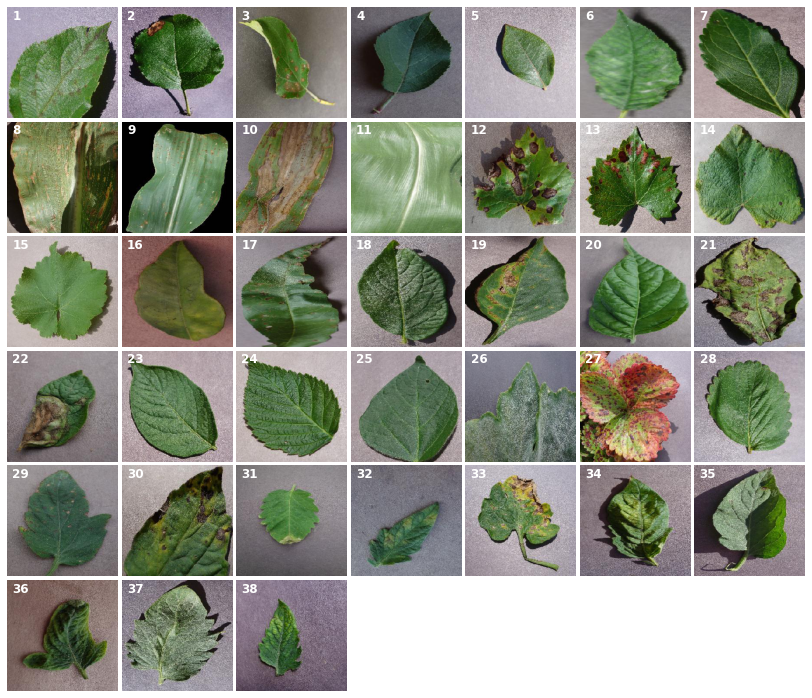
\includegraphics[scale=0.4]{png/image_per_specie.png}
\caption{The PlantVillage image dataset. This
dataset contains 38 categories of diseased or healthy leaf images}
\label{fig:data}
\end{figure} \noindent
(Figure \ref{fig:data}) and compared results of each model. This dataset comprises healthy  or diseased leaf images classified into $38$ labels, $42,754$ images, $14$ different crop species and $20$ different diseases including healthy ones. 
%Class names corresponding to each label are as follows: 1, Apple Apple scab; 2, Apple Black rot; 3, Apple Cedar apple rust; 4, Apple healthy; 5, Blueberry healthy; 6, Cherry (including sour) healthy; 7, Cherry (including sour) Powdery mildew; 8, Corn (maize) Cercospora leaf spot Gray leaf spot; 9, Corn (maize) Common rust; 10, Corn (maize) healthy; 11, Corn (maize) Northern Leaf Blight; 12, Grape Black rot; 13, Grape Esca (Black Measles); 14, Grape healthy; 15, Grape Leaf blight (Isariopsis Leaf Spot); 16, Orange Haunglongbing (Citrus greening); 17, Peach Bacterial spot; 18, Peach healthy; 19, Pepper, bell Bacterial spot; 20, Pepper, bell healthy; 21, Potato Early blight; 22, Potato healthy; 23, Potato Late blight; 24, Raspberry healthy; 25, Soybean healthy; 26, Squash Powdery mildew; 27, Strawberry healthy; 28, Strawberry Leaf scorch; 29, Tomato Bacterial spot; 30, Tomato Early blight; 31, Tomato healthy; 32, Tomato Late blight; 33, Tomato Leaf Mold; 34, Tomato Septoria leaf spot; 35, Tomato Spider mites Two-spotted spider mite; 36, Tomato Target Spot; 37, Tomato Tomato mosaic virus; and 38, Tomato Tomato Yellow Leaf Curl Virus. 
The dataset was split with $3,847$ images set out as validation set and $3,102$ images as test set, all images were reshaped into size $224\times 224\times 3$ since images usually comes in different sizes and a batch size of $64$ was used. Different variations of images in the dataset was created using different data augmentation techniques (flipping, zooming, rotating, warping, lightening), data augmentation is used to artificially create new data from the existing train dataset by creating modified version of the images with different amount of variances, this technique improves the training accuracy and helps the model generalize better from different variance added to the image {\cite{stephen2019efficient}}. 

% so as to pass different modified versions of the same image into the deep learning model and thereby improve the performance of the model. 


\begin{figure}[H]
\centering
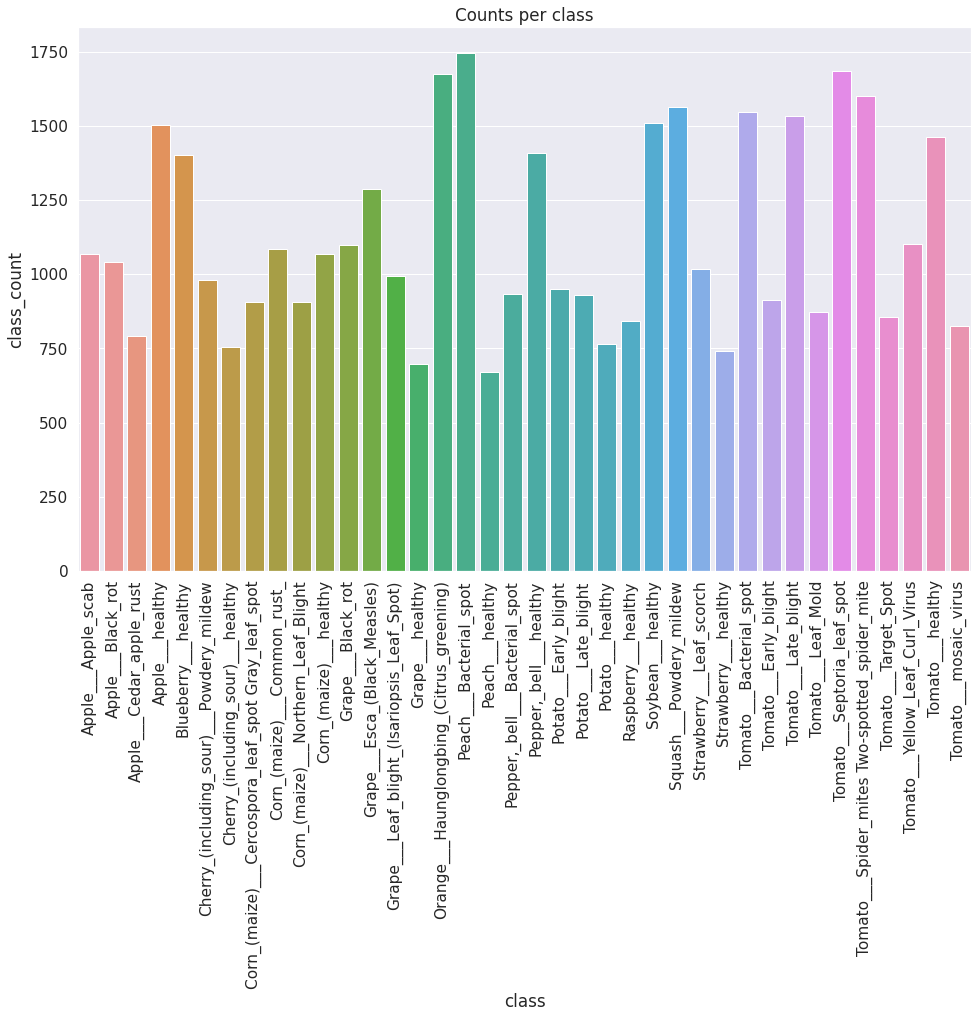
\includegraphics[scale=0.3]{png/counts_per_class.png}
\caption{Bar chart showing the number of images in each class}
\label{fig:count}
\end{figure} 

\section{Model Training}
Training the models was performed using Fastai deep learning library {\cite{Howard_2020}} and Pytorch deep leaning library {\cite{NEURIPS2019_9015}} on Python $3.7$, running on Google colab (\url{https://colab.research.google.com}) with the provided free GPU from colab, it took about $3$ to $6$ minutes to train the models per epoch. The network was initialized with random weights, using a categorical cross-entropy loss metric, network weights were optimized using the Adam optimization algorithm with a learning rate of $0.01$, a set of $64$ images with a size of $224 \times 224$ were fed to the network as a batch per iteration. A pseudo-random number was seeded to make sure the same weight values are initialised for each training instance, which makes sure results are reproducible for each trained model.



\section{Base Model Architecture}
A convolution neural network was built to learn the class where each image belongs to. The network consists of the input image, six convolution layers, two fully connected layers and the output layer (Figure \ref{fig:cnn_arch}). Each convolution layer was of kernel size $3 \times 3$, applied at stride $1$ and padding $1$, the number of kernels were $16,\;32,\;64\;,128\;,256\;,512$ respectively for each 
\begin{figure}[H]
\centering
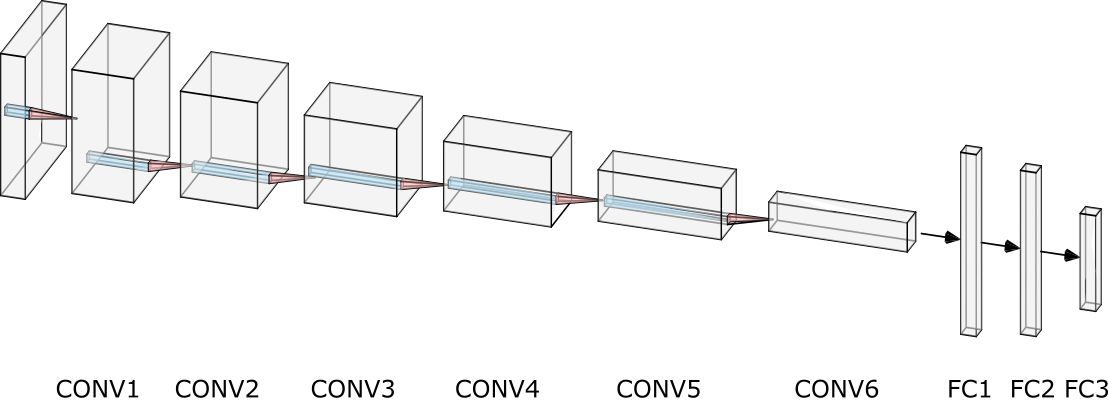
\includegraphics[scale=0.5]{png/drawing_nn.png}
\caption{Simplified base model architecture}
\label{fig:cnn_arch}
\end{figure} \noindent 
preceding convolution layer, batch normalisation was also added after each convolution layer to speed up training. To reduce dimensions of output features after each convolution layer, max pooling layers of kernel size $2 \times 2$, applied at stride $2$ and zero padding was added after each convolution layer (Table \ref{tab:cnn_arch}). Output image from the final max pool layer was flattened to a $1$D array and fed into fully connected layers with size $1024, \;, 512, \text{ and }, 38$ respectively, batch norm and dropout with rate $0.5$ was added to the first two fully connected layers. ReLU activation was used for all layers except the output layer which uses softmax to compute probabilities of an image belonging to a particular class. The model contained $6,841,766$ trainable parameters, batch size $64$ and learning rate $0.01$ was used during training. 


\begin{table}[H]
\centering
\begin{longtable}{c c A A}
\toprule
  & Type / Stride($s$) / Padding($p$) \; & \text{Filter Shape}\; & \text{Input Size}\;  \\ \midrule
 
CONV1 & Conv / $s=1$ / $p=1$     & 3 \times 3 \times 3 \times 16    & 224 \times 224 \times 3   \\
& Max Pool / $s=2$ / $p=0$ &     2 \times 2                   & 112 \times 112 \times 16 \\ %\pagebreak
CONV2 & Conv / $s=1$ / $p=1$     & 3 \times 3 \times 16 \times 32   & 112 \times 112 \times 16    \\
  & Max Pool / $s=2$ / $p=0$ &      2 \times 2  			    & 56 \times 56 \times 32 \\
CONV3 & Conv / $s=1$ / $p=1$     & 3 \times 3 \times 32 \times 64   & 56 \times 56 \times 32     \\
  & Max Pool / $s=2$ / $p=0$ &  2 \times 2 		   				& 28 \times 28 \times 64 \\
CONV4 & Conv / $s=1$ / $p=1$     & 3 \times 3 \times 64 \times 128  & 28 \times 28 \times 64     \\
  & Max Pool / $s=2$ / $p=0$ &  		2 \times 2			    & 14 \times 14 \times 128  \\
CONV5 & Conv / $s=1$ / $p=1$     & 3 \times 3 \times 128 \times 256 & 14 \times 14 \times 128  \\
  & Max Pool / $s=2$ / $p=0$ &     2 \times 2					& 7 \times 7 \times 256   \\
CONV6 & Conv / $s=1$ / $p=1$     & 3 \times 3 \times 256 \times 512 & 7 \times 7 \times 256   \\
  & Max Pool / $s=2$ / $p=0$ &  2 \times 2                      & 3 \times 3 \times 512   \\


FC1 & Fully Connected   & 4068 \times 1024  & 1 \times 1 \times 4068  \\ 
FC2 & Fully Connected   & 1024 \times 512   & 1 \times 1 \times 1024  \\
FC3 & Fully Connected   & 512 \times 38     & 1 \times 1 \times 512  \\ 
  & Softmax           & \text{Classifier} & 1 \times 1 \times 38 \\ \bottomrule
\end{longtable}
\caption{Base model architecture}
\label{tab:cnn_arch}
\end{table}



\section{Transfer Learning}
To improve training accuracy and speed up training time we adopt transfer learning. Transfer learning can be described as the improvement of learning of a new task by the transition of information from a previously learned similar task, model weights from pre-trained models created for large-scale image-classification datasets, such as ImageNet are reused to solve similar image-classification tasks. The following steps were taken to implement transfer learning:
\begin{enumerate}
\item Pre-train the source model on a source dataset. The pre-trained model and its parameters were downloaded and the source dataset used is the ImageNet dataset containing $1,000$ classes in our case.
\item Create a new neural network model, i.e., the target model. This replicates all model designs and their parameters on the source model, except the output layer. We assume that these model parameters contain the knowledge learned from the source dataset and this knowledge will be equally applicable to the target dataset. We also assume that the output layer of the source model is closely related to the labels of the source dataset and is therefore not used in the target model.
\item Add an output layer whose output size is the number of target dataset classes to the target model.
\item Train the target model on a target dataset. We would freeze the pre-trained layers and train the output layer from scratch, then unfreeze the pre-trained layers and jointly train both the pre-trained layers and the output layer of the target model with a much more smaller learning rate.
\end{enumerate} \noindent
VGG16 and ResNext-50 were used as the pre-trained models in this project. 

\subsection{VGG16}
VGG16 {\cite{simonyan2015deep}} model achieved $7.1\%$ top-5 error rate in the ImageNet dataset and came second for classification in the ILSVRC 2014 challenge. It makes the improvement over AlexNet {\cite{Krizhevsky}} by replacing large kernel-sized filters ($11$ and $5$ in the first and second convolutional layer respectively) with stacks of $3 \times 3$ kernel-sized filters. Each stack of  $3 \times 3$ convolutional layer with stride $1$, pad $1$ and different depths is followed by $2 \times 2$ max pooling layers applied at stride $2$, three fully-connected (FC) layers follow the final max pool layer; the first two have 4096 channels each, the third performs 1000-way ILSVRC classification and thus contains 1000 channels (one for each class), the final layer is the softmax layer and ReLU is applied to all hidden layers (Figure \ref{fig:vgg16_arch}). It was shown that the added depth and smaller filters is beneficial for classification accuracy.

\begin{figure}[H]
\centering
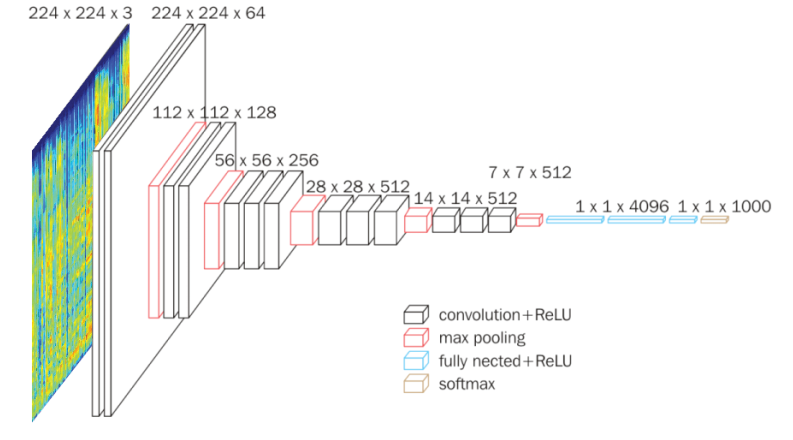
\includegraphics[scale=0.8]{png/vgg16.png}
\caption[VGG16 model architecture]{VGG16 model architecture, \protect{\cite{Das2019DoubleCV}}}	
\label{fig:vgg16_arch}
\end{figure} 



\subsection{ResNext-50}
With the success of plain deep networks such as VGG16, the knee-jerk reaction would be to build even more deeper networks (simply stacking more convolutional and pooling layers) in order to improve prediction results, but a $20$-layer plain network got lower training error and test error than $56$-layer plain network when trained with the CIFAR-10 dataset {\cite{He2015DeepRL}}. Deep networks are in fact susceptible to vanishing/exploding gradients, making it harder to optimise compared to shallow networks. During backpropagation, deriving partial derivative of the error function with respect to the current weight in each iteration of training, has the effect of multiplying $n$ of these small/large numbers to compute gradients of intermediate layers in an $n$-layer network. For deeper networks, multiplying $n$ of these small numbers will become zero (vanished), while multiplying $n$ of these large numbers will become too large (exploded).

Residual learning introduced in ResNet architecture {\cite{He2015DeepRL}} tackles the problem stated above by using network layers to fit a residual mapping using skip connections instead of directly trying to fit a desired underlying mapping, i.e., for the output $H(\bm{x})= F(\bm{x}) + \bm{x}$, use weight layers to learn residual mapping: $F(\bm{x}) = H(\bm{x})-\bm{x}$ (Figure \ref{subfig:residual_block}) as we move to the next layer, instead of desired function $H(\bm{x})$ directly.
\begin{figure}[H]
\centering
	\begin{subfigure}[t]{\textwidth}
	\centering
	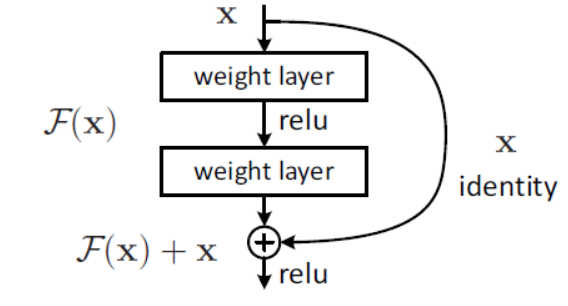
\includegraphics[scale=0.7]{png/residual_block.png}
 	\caption{A residual block}	 
	\label{subfig:residual_block}
	\end{subfigure}
	
	\medskip
	
	\begin{subfigure}[t]{\textwidth}
	\centering
	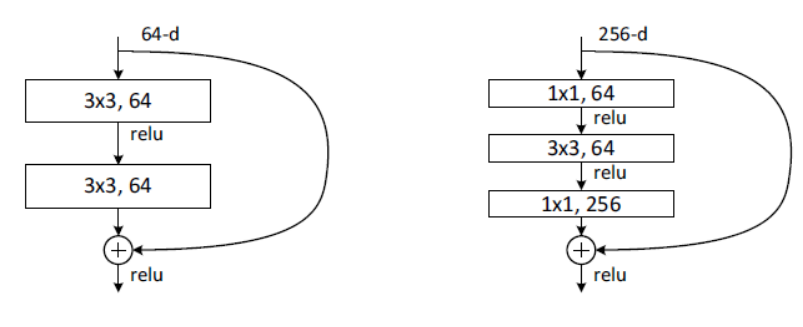
\includegraphics[scale=0.7]{png/bottleneck.png}		
	\caption{A bottleneck building block for ResNet-50/101/152}	 
	\label{subfig:bottleneck}
	\end{subfigure}
\caption[Residual learning blocks]{Residual learning blocks, \protect{\cite{He2015DeepRL}}}	 
\label{fig:residual_learning}
\end{figure} \noindent
ResNet architecture consists of a $7 \times 7$ convolutional layer, $2 \times 2$ pooling layer, stacks of residual blocks with two $3 \times 3$ convolutional layers, number of filters are double after each block, and the layers are down-sampled spatially using stride $2$ and a global average pooling layer after the last convolutional layer. The final output is the only fully connected layer in the network, batch norm was added after every convolutional layer. For deep residual networks, $1 \times 1$ convolutional layers (bottlenecks) are added to the start and end of residual blocks (Figure \ref{subfig:bottleneck}) to improve efficiency. Adding bottlenecks is a technique suggested in  GoogLeNet {\cite{szegedy2015going}} (Inception-v1). The $1 \times 1$ convolutional layers reduces the number of connections (parameters) since it's only computation occurs on the channel dimension, while not degrading the performance of the network. ResNet won the ILSVRC 2015 in image classification, detection, and localization with $3.57\%$ top-$5$ error rate (with ensembles).

{\cite{zagoruyko2017wide}} argued that residual blocks are more important than depth, hence, wide residual networks were introduced, where filter size for residual blocks where increased by factors of $k$ ($F \times k$ filters instead of $F$ filters in each layer). It was also showed that increasing width instead of depth is more computationally efficient. Wide 50-layer residual networks outperforms 152-layer ResNet when trained on the ImageNet dataset $6.03\%$ versus $6.16\%$ top-5 error rate. 

ResNext {\cite{Xie}} tried to improve wide ResNet by increasing width of the residual blocks through multiple parallel pathways. Multiple residual blocks with bottlenecks are stacked in parallel with $d$ internal dimension for each path and $c$ total number of pathways, called cardinality (Figure \ref{fig:resnext}). The architecture for ResNext-50 is the same as ResNet-50 but with the extra parallel pathways in the residual blocks, it achieved a $6.6\%$ top-5 error rate when trained on the ImageNet dataset with $1,000$ classes compared to a $8.2\%$ error rate for ResNet-50 on the same dataset.
\begin{figure}[H]
\centering
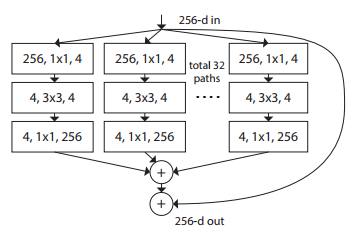
\includegraphics[scale=1.1]{png/resnext.png}
\caption[A block of ResNeXt with cardinality = 32]{A block of ResNeXt with cardinality $= \;32$, \protect{\cite{Xie}}}	
\label{fig:resnext}
\end{figure} 



\section{Results}
In this section, results gotten on validation data are compared for the three different models studied in this research; a base CNN model, a VGG16 model and a ResNext-50 $32\times 4d$ model, evaluation metrics used are also defined. Performance measures such as accuracy, precision, recall, and f1 score are defined by using four features; true positive ($tp_i$) - correctly identified prediction for each class, true negative ($tn_i$) - correctly rejected prediction for certain class, 
 \begin{table}[H]
\centering
\begin{tabular}{c A A A A A}
%\\setlength{\tabcolsep}{12pt} default is 6 pt
 & & \multicolumn{4}{c}{\text{Predicted class}} \\
\toprule
 &                & \text{A}\; & \text{B}\; & \text{C}\; & \text{D}\; \\ \midrule
\multirow{4}*{Actual  class} & \text{A}  & 9 & \cellcolor{brown!55} 1  & \cellcolor{brown!55} 0  & \cellcolor{brown!55} 0  \\
 				  & \text{B}  			 & \cellcolor{red!55} 1 & \cellcolor{blue!55} 15 & \cellcolor{blue!55} 3  & \cellcolor{blue!55} 1  \\ 
                  & \text{C}  			 & \cellcolor{red!55} 5 & \cellcolor{blue!55} 0  & \cellcolor{blue!55} 24 & \cellcolor{blue!55} 1  \\
                  & \text{D}  			 & \cellcolor{red!55} 0 & \cellcolor{blue!55} 4  & \cellcolor{blue!55} 1  & \cellcolor{blue!55} 15  \\ \bottomrule
\end{tabular}
\caption[Confusion matrix for $4$-class classification]{Confusion matrix for $4$-class classification. The blue, red, and brown cells shows $tn$, $fp$, and $fn$ values respectively for class $A$, matrix diagonal shows $tp$ values for each class.}
\label{tab:confusion}
\end{table} \noindent
false positive ($fp_i$) - incorrectly identified predictions for certain class, and false negative ($fn_i$) - incorrectly rejected data for certain class, of class $C_i$, these four features can be gotten from the confusion matrix (Table \ref{tab:confusion}). Weighted average was used for all performance measure, except accuracy, because it factors in weight that depends on the number of true labels of each class which gives a better picture for imbalanced datasets. The performance measures are defined as follows:
\begin{itemize}
\item[-] Accuracy: Accuracy is the ratio of correctly predicted observation to the total observations. It is not a good measure for imbalanced dataset i.e., dataset with uneven class distribution, since it does not distinguish between the numbers of correctly classified examples of different classes, it is given by:
\begin{equation}\label{eqn:acccuracy}
\text { Accuracy }= \displaystyle \frac{\sum_{i=1}^{m} \dfrac{tp_{i}}{tp_{i} + fp_{i} + fn_{i} + tn_{i}}}{m}
\end{equation}

\item[-] Top-3 Accuracy: Top-3 accuracy takes the $3$ model predictions with higher probabilities, if one of them is a true label, it classifies the prediction as correct. Accuracy is a particular situation where only the highest probability prediction is taken into consideration.

\item[-] Precision: Precision is the ratio of correctly predicted positive observations to the total predicted positive observations. This metric answers the question: of all image labelled as being to a class, how many are actually in that class, it is given by:
% Effectiveness of a classifier to identify class labels if calculated from sums of per-text decisions 
\begin{equation}\label{eqn:precision}
\text{Precision}_{\text{Weighted}} = \displaystyle \frac{\sum_{i=1}^{m}\left(\left|y_{i}\right| \dfrac{tp_{i}}{tp_{i} + fp_{i}}\right)}{\sum_{i=1}^{m}\left|y_{i}\right|}  
\end{equation}

\item[-]  Recall or sensitivity: Recall is the ratio of correctly predicted positive observations to the all observations in actual class. The metric answers the question: of all the images belonging to a class, how many were labelled, it is given by:
% Effectiveness of a classifier to identify positive labels
\begin{equation}\label{eqn:recall}
\text{Recall}_{\text{Weighted}} = \displaystyle \frac{\sum_{i=1}^{m}\left(\left|y_{i}\right| \dfrac{tp_{i}}{tp_{i} + fn_{i}}\right)}{\sum_{i=1}^{m}\left|y_{i}\right|} 
\end{equation}

\item[-] F1 score: F1 Score is the weighted average of precision and recall, it is usually more useful than accuracy, especially for uneven class distribution, it is given by:
% Relations between data's positive labels and those given by a classifier
\begin{equation}\label{eqn:f1-score}
\text {F1 score}_{\text {Weighted}} = \displaystyle \frac{\sum_{i=1}^{m}\left(\left|y_{i}\right| \dfrac{2 tp_{i}}{2 tp_{i} + fp_{i} + fn_{i}}\right)}{\sum_{i=1}^{m}\left|y_{i}\right|}
\end{equation}
\end{itemize} \noindent 
where $y_i$ is the number of instances for class $i$. Table \ref{tab:result} shows the results gotten for each model. 

% weighted 
%  However, if N accuracy increases significantly, we can find that it is actually learning but is lacking some fine-tuning

\begin{table}[H]
\centering
\begin{tabular}{A A A A A A}
\toprule
 & \text{Accuracy}\; & \text{Top-3 Accuracy}\; & \text{Precision}\; & \text{Recall}\; & \text{F1 score}\; \\ \midrule
 
\text{Base Model}  & 0.9277 & 0.9923 & 0.9329 & 0.9277 & 0.9277 \\
\text{VGG16}       & 0.9821 & 0.9995 & 0.9853 & 0.9821 & 0.9819 \\ 
\text{ResNext-50}   & 0.9823 & 1.00   & 0.9850 & 0.9823 & 0.9822 \\ \bottomrule
\end{tabular}
\caption{Comparing different evaluation metrics for the models studied on  validation data}
\label{tab:result}
\end{table} \noindent
Visualisation of the model was carried out using the cross-entropy (or logistic) loss defined in Equation \ref{eqn:cost}, loss of the model decreases as training is done (Figure \ref{fig:models_loss}). ResNext-50 has the best performance since training loss and validation loss converges, with minimal space in between both curves as the model trains, the base model performs worst. 

\begin{figure}[H]
\begin{subfigure}[t]{.5\textwidth}
\centering
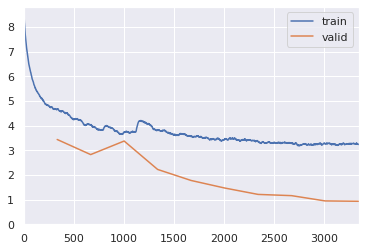
\includegraphics[scale=0.6]{png/base_model_loss.png}
\caption{Base model training loss}
\label{subfig:base_loss}
\end{subfigure}
\hfill
\begin{subfigure}[t]{.5\textwidth}
\centering
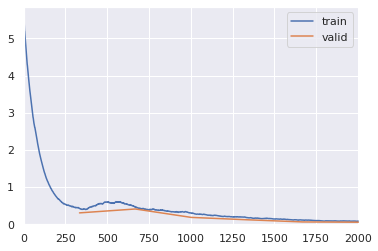
\includegraphics[scale=0.6]{png/vgg_loss.png}
\caption{VGG16 training loss}
\label{subfig:vgg_loss}
\end{subfigure}
\medskip
\begin{subfigure}[t]{\textwidth}
\centering
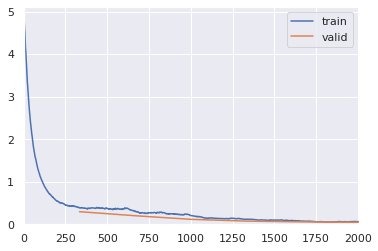
\includegraphics[scale=0.6]{png/resnext_loss.png}
\caption{ResNext-50 training loss}
\label{subfig:resnext_loss}
\end{subfigure}
\caption[Training loss for different models]{Training loss for different models, the horizontal axes denotes number of epochs, while the vertical axes denotes loss}
\label{fig:models_loss}
\end{figure} \noindent
Confusion matrices are used to visualise more outputs (Figure \ref{fig:confusion_matrix}). Most confused prediction pair for VGG16 and ResNext50 are the same; tomato healthy and apple scab with $45$ incorrectly identified predictions, while for the base model, tomato yellow leaf and tomato bacterial spot with $86$ incorrectly identified predictions is the most confused prediction pair.  

\begin{figure}[H]
\begin{subfigure}[t]{.5\textwidth}
\centering
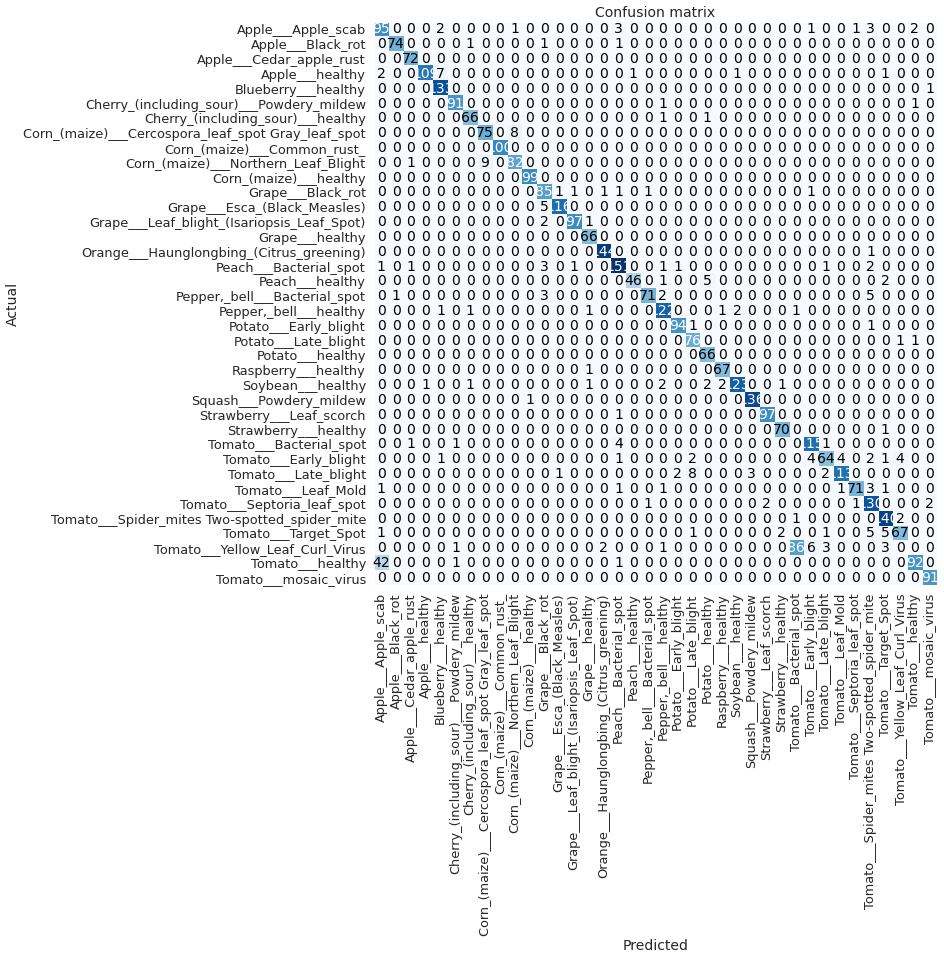
\includegraphics[width=7cm,height=7cm]{png/base_confusion_matrix.png}
\caption{Base model confusion matrix}
\label{subfig:base_confusion}
\end{subfigure}
\hfill
\begin{subfigure}[t]{.5\textwidth}
\centering
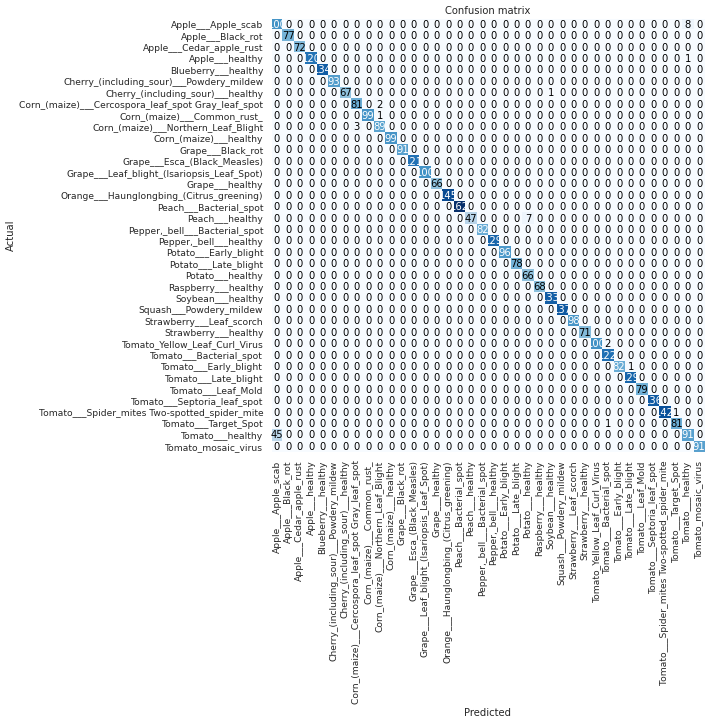
\includegraphics[width=7cm,height=7cm]{png/vgg16_confusion_matrix.png}
\caption{VGG16 confusion matrix}
\label{subfig:vgg_confusion}
\end{subfigure}
\medskip
\begin{subfigure}[t]{\textwidth}
\centering
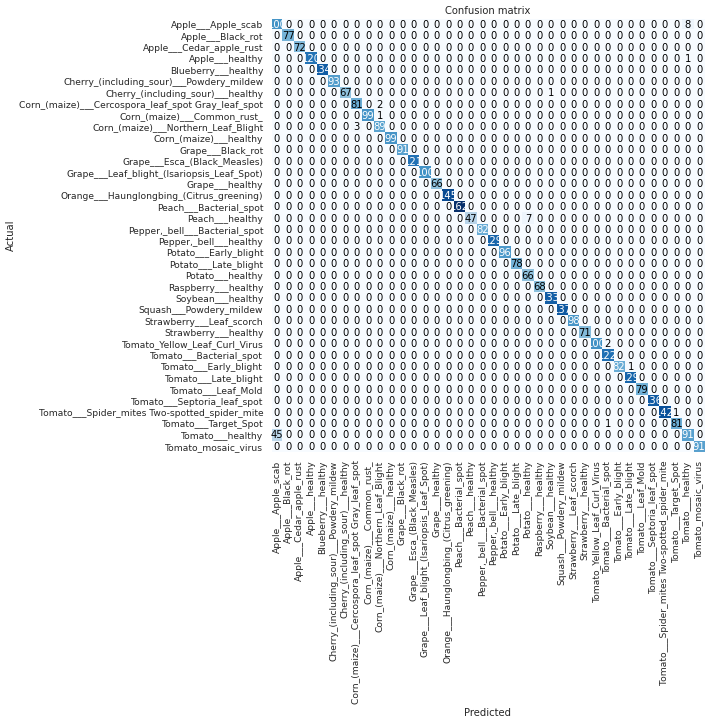
\includegraphics[width=7cm,height=7cm]{png/resnext50_confusion_matrix.png}
\caption{ResNext-50 confusion matrix}
\label{subfig:resnext_confusion}
\end{subfigure}
\caption[Confusion matrix for different models]{Confusion matrix for different models, thicker colours signifies better accuracy}
\label{fig:confusion_matrix}
\end{figure}





\chapter{Conclusion}
In this project, we implemented convolutional neural networks to classify plant leaf diseases using images of healthy and diseased leaves reaching an accuracy of $98\%$. In Chapter 1, we defined basic terms and gave corresponding results, then a binary classification problem was introduced and how to solve the problem using logistic regression. It is difficult to solve binary classification problem where the two classes can not be separated by a hyperplane using standard machine learning algorithms, so we introduced multi layer perceptrons (neural networks) to solve this problem. Basic optimisation and regularisation algorithms for neural networks was also introduced in this chapter.

In Chapter 2, we reviewed advancements in neural network architectures and how better computer power has helped accelerate research into the field due to high computational demands of training neural networks. We also reviewed areas of agriculture where deep learning has been applied with good accuracy and generalisation, from plant phenotyping and yield prediction, to weed management and pest control, and crop diseases. These high quality models has helped improved agricultural produce yield and improved efficiency of solving different problems faced in the agricultural process.

In Chapter 3, we took a deep dive into training neural networks (convolutional neural networks in particular), first looking at some different activation functions which introduces non-linearity to the network. Then moving on to explain the backpropagation algorithm which forms the basis of training and optimising neural networks. Building blocks of convolutional neural networks were then investigated, and finally modern methods for optimising and regularising these networks were studied.

Chapter 4 deals with the main problem statement, which consists of identifying healthy and diseased crop plants using convolution neural networks. Three different models were trained on the dataset - a custom built base model and two popular models (VGG16 and ResNext-50). The popular models were studied in detail, considering mainly it's architectures and what makes them achieve state of the art result. Finally, we compare and visualise results from the three models, with ResNext-50 having the best all round performance.

The results gotten from this project could be improved upon by making ensembles of the different models, we aim to study this problem further. Also, more applications of deep learning in agriculture can be studied, for example, fine mapping of key soil nutrients using high resolution remote sensing image with convolutional neural networks.
	



\newpage
\addcontentsline{toc}{chapter}{References}
\renewcommand{\bibname}{\centering References}
 \bibliographystyle{apalike}
 
 
 
 \bibliography{bib/alliref}

%\addtocontents{toc}{\protect\renewcommand{\protect\numberline}[1]{}}
%\includepdf[pages=1, offset=70 -70, delta=70 -70, 
%			addtotoc={1,chapter,1,Appendix,sec:appendix},										pagecommand={\section*{\centering Appendix}}]  
%     		{pdf/fastai_plant_disease.pdf}
%\includepdf[pages=2-, offset=75 -75, delta=75 -75,  										pagecommand={}]  
%    	{pdf/fastai_plant_disease.pdf}




\nocite{*}

% \nocite{MatrixCalculus}
% \nocite{guarav}
% \nocite{pmlr-v15-glorot11a}
% \nocite{10.5555/1162264}
% \nocite{zhang2020dive}
% \nocite{behera2019performance}








\end{document}
